% Options for packages loaded elsewhere
\PassOptionsToPackage{unicode}{hyperref}
\PassOptionsToPackage{hyphens}{url}
%
\documentclass[
]{book}
\usepackage{lmodern}
\usepackage{amssymb,amsmath}
\usepackage{ifxetex,ifluatex}
\ifnum 0\ifxetex 1\fi\ifluatex 1\fi=0 % if pdftex
  \usepackage[T1]{fontenc}
  \usepackage[utf8]{inputenc}
  \usepackage{textcomp} % provide euro and other symbols
\else % if luatex or xetex
  \usepackage{unicode-math}
  \defaultfontfeatures{Scale=MatchLowercase}
  \defaultfontfeatures[\rmfamily]{Ligatures=TeX,Scale=1}
\fi
% Use upquote if available, for straight quotes in verbatim environments
\IfFileExists{upquote.sty}{\usepackage{upquote}}{}
\IfFileExists{microtype.sty}{% use microtype if available
  \usepackage[]{microtype}
  \UseMicrotypeSet[protrusion]{basicmath} % disable protrusion for tt fonts
}{}
\makeatletter
\@ifundefined{KOMAClassName}{% if non-KOMA class
  \IfFileExists{parskip.sty}{%
    \usepackage{parskip}
  }{% else
    \setlength{\parindent}{0pt}
    \setlength{\parskip}{6pt plus 2pt minus 1pt}}
}{% if KOMA class
  \KOMAoptions{parskip=half}}
\makeatother
\usepackage{xcolor}
\IfFileExists{xurl.sty}{\usepackage{xurl}}{} % add URL line breaks if available
\IfFileExists{bookmark.sty}{\usepackage{bookmark}}{\usepackage{hyperref}}
\hypersetup{
  pdftitle={Life2 Code Compendium},
  pdfauthor={Derek McCrae Norton},
  hidelinks,
  pdfcreator={LaTeX via pandoc}}
\urlstyle{same} % disable monospaced font for URLs
\usepackage{color}
\usepackage{fancyvrb}
\newcommand{\VerbBar}{|}
\newcommand{\VERB}{\Verb[commandchars=\\\{\}]}
\DefineVerbatimEnvironment{Highlighting}{Verbatim}{commandchars=\\\{\}}
% Add ',fontsize=\small' for more characters per line
\usepackage{framed}
\definecolor{shadecolor}{RGB}{248,248,248}
\newenvironment{Shaded}{\begin{snugshade}}{\end{snugshade}}
\newcommand{\AlertTok}[1]{\textcolor[rgb]{0.94,0.16,0.16}{#1}}
\newcommand{\AnnotationTok}[1]{\textcolor[rgb]{0.56,0.35,0.01}{\textbf{\textit{#1}}}}
\newcommand{\AttributeTok}[1]{\textcolor[rgb]{0.77,0.63,0.00}{#1}}
\newcommand{\BaseNTok}[1]{\textcolor[rgb]{0.00,0.00,0.81}{#1}}
\newcommand{\BuiltInTok}[1]{#1}
\newcommand{\CharTok}[1]{\textcolor[rgb]{0.31,0.60,0.02}{#1}}
\newcommand{\CommentTok}[1]{\textcolor[rgb]{0.56,0.35,0.01}{\textit{#1}}}
\newcommand{\CommentVarTok}[1]{\textcolor[rgb]{0.56,0.35,0.01}{\textbf{\textit{#1}}}}
\newcommand{\ConstantTok}[1]{\textcolor[rgb]{0.00,0.00,0.00}{#1}}
\newcommand{\ControlFlowTok}[1]{\textcolor[rgb]{0.13,0.29,0.53}{\textbf{#1}}}
\newcommand{\DataTypeTok}[1]{\textcolor[rgb]{0.13,0.29,0.53}{#1}}
\newcommand{\DecValTok}[1]{\textcolor[rgb]{0.00,0.00,0.81}{#1}}
\newcommand{\DocumentationTok}[1]{\textcolor[rgb]{0.56,0.35,0.01}{\textbf{\textit{#1}}}}
\newcommand{\ErrorTok}[1]{\textcolor[rgb]{0.64,0.00,0.00}{\textbf{#1}}}
\newcommand{\ExtensionTok}[1]{#1}
\newcommand{\FloatTok}[1]{\textcolor[rgb]{0.00,0.00,0.81}{#1}}
\newcommand{\FunctionTok}[1]{\textcolor[rgb]{0.00,0.00,0.00}{#1}}
\newcommand{\ImportTok}[1]{#1}
\newcommand{\InformationTok}[1]{\textcolor[rgb]{0.56,0.35,0.01}{\textbf{\textit{#1}}}}
\newcommand{\KeywordTok}[1]{\textcolor[rgb]{0.13,0.29,0.53}{\textbf{#1}}}
\newcommand{\NormalTok}[1]{#1}
\newcommand{\OperatorTok}[1]{\textcolor[rgb]{0.81,0.36,0.00}{\textbf{#1}}}
\newcommand{\OtherTok}[1]{\textcolor[rgb]{0.56,0.35,0.01}{#1}}
\newcommand{\PreprocessorTok}[1]{\textcolor[rgb]{0.56,0.35,0.01}{\textit{#1}}}
\newcommand{\RegionMarkerTok}[1]{#1}
\newcommand{\SpecialCharTok}[1]{\textcolor[rgb]{0.00,0.00,0.00}{#1}}
\newcommand{\SpecialStringTok}[1]{\textcolor[rgb]{0.31,0.60,0.02}{#1}}
\newcommand{\StringTok}[1]{\textcolor[rgb]{0.31,0.60,0.02}{#1}}
\newcommand{\VariableTok}[1]{\textcolor[rgb]{0.00,0.00,0.00}{#1}}
\newcommand{\VerbatimStringTok}[1]{\textcolor[rgb]{0.31,0.60,0.02}{#1}}
\newcommand{\WarningTok}[1]{\textcolor[rgb]{0.56,0.35,0.01}{\textbf{\textit{#1}}}}
\usepackage{longtable,booktabs}
% Correct order of tables after \paragraph or \subparagraph
\usepackage{etoolbox}
\makeatletter
\patchcmd\longtable{\par}{\if@noskipsec\mbox{}\fi\par}{}{}
\makeatother
% Allow footnotes in longtable head/foot
\IfFileExists{footnotehyper.sty}{\usepackage{footnotehyper}}{\usepackage{footnote}}
\makesavenoteenv{longtable}
\usepackage{graphicx,grffile}
\makeatletter
\def\maxwidth{\ifdim\Gin@nat@width>\linewidth\linewidth\else\Gin@nat@width\fi}
\def\maxheight{\ifdim\Gin@nat@height>\textheight\textheight\else\Gin@nat@height\fi}
\makeatother
% Scale images if necessary, so that they will not overflow the page
% margins by default, and it is still possible to overwrite the defaults
% using explicit options in \includegraphics[width, height, ...]{}
\setkeys{Gin}{width=\maxwidth,height=\maxheight,keepaspectratio}
% Set default figure placement to htbp
\makeatletter
\def\fps@figure{htbp}
\makeatother
\setlength{\emergencystretch}{3em} % prevent overfull lines
\providecommand{\tightlist}{%
  \setlength{\itemsep}{0pt}\setlength{\parskip}{0pt}}
\setcounter{secnumdepth}{5}
\usepackage{booktabs}
\usepackage[]{natbib}
\bibliographystyle{apalike}

\title{Life2 Code Compendium}
\author{Derek McCrae Norton}
\date{2021-05-18}

\begin{document}
\maketitle

{
\setcounter{tocdepth}{1}
\tableofcontents
}
\hypertarget{intro}{%
\chapter{Introduction}\label{intro}}

This document is intended to catalog and document all of the code for Life2 as well as how to use it.

\hypertarget{locations}{%
\section{Locations}\label{locations}}

All code is currently versioned using SVN and can be found here:

\begin{longtable}[]{@{}ll@{}}
\toprule
Solution & Location\tabularnewline
\midrule
\endhead
GBA & \url{http://06eyrad:81/svn/GBA}\tabularnewline
St Francis & \url{http://06eyrad:81/svn/st_francis}\tabularnewline
HL7 & \url{http://06eyrad:81/svn/HL7}\tabularnewline
stac & \url{http://06eyrad:81/svn/stac}\tabularnewline
\bottomrule
\end{longtable}

\hypertarget{general-notes}{%
\section{General notes}\label{general-notes}}

\begin{itemize}
\item
  Currently Imidex does development in Eclipse using StatET. \texttt{.project} files are for that and not RStudio.
\item
\end{itemize}

\hypertarget{bookdown-info}{%
\section{Bookdown Info}\label{bookdown-info}}

Remember each Rmd file contains one and only one chapter, and a chapter is defined by the first-level heading \texttt{\#}.

To compile this example to PDF, you need XeLaTeX. You are recommended to install TinyTeX (which includes XeLaTeX): \url{https://yihui.org/tinytex/}.

\hypertarget{gba}{%
\chapter{Georgia Bankers Association}\label{gba}}

This document is intended to catalog and document all of the code for GBA as well as how to use it.

\hypertarget{notes-questions}{%
\section{Notes / Questions}\label{notes-questions}}

\begin{itemize}
\tightlist
\item
  \texttt{futile.logger} is used for logging
\item
  What are the following datasets?

  \begin{itemize}
  \tightlist
  \item
    AHH
  \item
    VBA - Claims processing company \url{https://vbasoftware.com/}
  \item
    XRF
  \end{itemize}
\item
  Modeling is currently done with \texttt{randomForest}, but this is a memory hog. Investigate other options such as \texttt{xgboost} or maybe \texttt{lightgbm}.
\item
  Look into another option for parameters. \texttt{config} package?
\item
  Packages are loaded way too many times. Each separate function seems to load a package. Should be able to fix by creating a package and not sourcing functions.
\item
  There are many used packages with no real way to ensure versioning. Maybe use \texttt{renv}?
\item
  iRollDT does a lot of work\ldots{} Examine
\item
  Date conversions with as.POSIXct seem very slow.
\item
  Futile Logger needs something to show section changes\ldots{} **** SECTION ****?
\end{itemize}

\hypertarget{project-structure}{%
\section{Project Structure}\label{project-structure}}

\hypertarget{ini-file}{%
\section{\texorpdfstring{\texttt{.ini} File}{.ini File}}\label{ini-file}}

This file contains all the needed parameters to create and run models.

\begin{verbatim}
#
#  Location to the GBA project
#
project_directory=E:/GCM/workspace/GBA
#
#   The working directory where intermediate preprocessed files
#   are stored. (switch to your local copy)
#
working_directory=C:/R/GCM/GBA/DEV
#
#   The location for the archive directory, where RDS
#   files used for production debugging is stored.  You
#   may want to create a process to clean up this directory
#   from time to time.
#
archive_dir=E:/GBA_temp/archive
#
#   The SQL user user ID used to connect to all of the database
#   DSN's below.
#
db_uid=R_user
#
#  The password to use to connect to all the database DSN's below
#
db_pwd=8ASjKj9shn
#
#   The SQL server DSN containing the raw production input data that 
#   is to be preprocessed and run through the models
#
db_dsn=GBA
#
#   The SQL server DSN for the database containing the external data
#
external_data_dsn=EXTERNAL_DATA
#
#   The SQL server DSN for the database where all the model output
#   is stored and that is used by the web user interface.
#
web_dsn=GBA_WEB
#
#  If in production, set live_data to TRUE.  For develop, set to FALSE.
#
live_data=FALSE
#
#  The number of days from the current date to process the predictions.  
#  Normally this should be -1, to indicate yesterday.
#
offset_days=-1
#
#   The working directory where intermediate preprocessed files
#   are stored.
#
rds_directory=C:/R/GCM/GBA/RDS
#
#  Where the GBA data has been FTP'd to and unzipped
#
raw_data_directory=G:/Paragon
#
#  dataset preprocessing settings
#
periodicity_days=13
fix_sample_times=FALSE
dev_start_date=2016-01-01
dev_end_date=2021-02-01
sample_from=policy_start_date
sample_to=policy_end_date
#
#  log file settings
#
log_level=DEBUG
log_file=GBA.log
\end{verbatim}

\hypertarget{r-code}{%
\section{\texorpdfstring{\texttt{R} Code}{R Code}}\label{r-code}}

\hypertarget{r}{%
\subsection{\texorpdfstring{\texttt{/R}}{/R}}\label{r}}

\hypertarget{main.r}{%
\subsubsection{\texorpdfstring{\texttt{main.R}}{main.R}}\label{main.r}}

\begin{itemize}
\tightlist
\item
  \texttt{get\_params()} - Configuration / Initialization settings to build the GBA and model
\item
  \texttt{connect\_to\_dbs()} - Connect to databases
\item
  \texttt{get\_params\_from\_file()} - Loads the parameter object from an initialization file.
\item
  \texttt{prompt\_for\_ini\_location()} - Prompt the user for the location of their initialization file. Verifies the user input that the file exists.
\item
  \texttt{load\_libraries()} - Loads the \texttt{imidexR2} package and iteratively loads functions from the \texttt{R} subfolders.
\item
  \texttt{set\_params\_datetime()} - Function used to modify the date and time in the parameters object, used to determine the demarcation point where the data is truncated.
\item
  \texttt{set\_working\_directory()} - Function used to set the RDS directory on the params object, including locations to X and Y dataset files.
\item
  \texttt{setup\_logging()} - Sets up the futile logger
\end{itemize}

\hypertarget{rmodel}{%
\subsection{\texorpdfstring{\texttt{/R/model}}{/R/model}}\label{rmodel}}

\hypertarget{build.r}{%
\subsubsection{\texorpdfstring{\texttt{build.R}}{build.R}}\label{build.r}}

\begin{itemize}
\tightlist
\item
  \texttt{build\_ed\_visit\_models\_version()} - Build models for future ED visits for specified DEV version
\item
  \texttt{build\_dx\_residual\_codes\_illness\_models\_version()} - Build models for primary diagnosis category residual codes, unclassified, all E codes, 259 and 260 for specified DEV version
\item
  \texttt{build\_dx\_health\_status\_illness\_models\_version()} - Build models for primary diagnosis category illdefinied conditions and factors influencing health status for specified DEV version
\item
  \texttt{build\_dx\_mental\_illness\_models\_version()} - Build models for primary diagnosis category mental illness for specified DEV version
\item
  \texttt{build\_dx\_congenital\_models\_version()} - Build models for primary diagnosis category congenital anomalies for specified DEV version
\item
  \texttt{build\_dx\_pregnancy\_models\_version()} - Build models for primary diagnosis category complications of pregnancy, childbirth, and the puerperium for specified DEV version
\item
  \texttt{build\_dx\_perinatal\_models\_version()} - Build models for primary diagnosis category conditions originating in the perinatal period for specified DEV version
\item
  \texttt{build\_dx\_endocrine\_models\_version()} - Build models for primary diagnosis category endocrine, nutritional, and metabolic diseases and immunity disorders for specified DEV version
\item
  \texttt{build\_dx\_injury\_models\_version()} - Build models for primary diagnosis category injury and poisoning for specified DEV version
\item
  \texttt{build\_dx\_neoplasms\_models\_version()} - Build models for primary diagnosis category neoplasms for specified DEV version
\item
  \texttt{build\_dx\_infectious\_models\_version()} - Build models for primary diagnosis category infectious and parasitic diseases for specified DEV version
\item
  \texttt{build\_dx\_genitourinary\_models\_version()} - Build models for primary diagnosis category diseases of the genitourinary system for specified DEV version
\item
  \texttt{build\_dx\_blood\_models\_version()} - Build models for primary diagnosis category diseases of the blood and bloodforming organs for specified DEV version
\item
  \texttt{build\_dx\_circulatory\_models\_version()} - Build models for primary diagnosis category diseases of the circulatory system for specified DEV version
\item
  \texttt{build\_dx\_nerve\_models\_version()} - Build models for primary diagnosis category diseases of the nervous system and sense organs for specified DEV version
\item
  \texttt{build\_dx\_musculoskeletal\_models\_version()} - Build models for primary diagnosis category diseases of the musculoskeletal system and connective tissue for specified DEV version
\item
  \texttt{build\_dx\_skin\_models\_version()} - Build models for primary diagnosis category diseases of the skin and subcutaneous tissue
\item
  \texttt{build\_dx\_digestive\_models\_version()} - Build models for primary diagnosis category diseases of the digestive system for specified DEV version
\item
  \texttt{build\_dx\_respiratory\_models\_version()} - Build models for primary diagnosis category diseases of the respiratory system for specified DEV version
\item
  \texttt{build\_med\_claim\_models\_version()} - Build models for med claim paid amts for specified DEV version
\item
  \texttt{build\_hospitalization\_event\_models\_version()} - Build models for hospitalization events for specified DEV version
\item
  \texttt{build\_change\_in\_total\_paid\_amt\_models()} - TODO
\item
  \texttt{build\_med\_claim\_models()} - TODO
\item
  \texttt{build\_hospitalization\_event\_models()} - TODO
\item
  \texttt{build\_models()} - Builds all of the GBA models
\item
  \texttt{rebuild\_models()} - Rebuilds models based on prior variables that were selected. Eliminates vars with a negative MSE. While this works, it did not show to improve model performance.
\item
  \texttt{get\_blocked\_variables()} - List of variables to exclude as candidate predictor variables.
\item
  \texttt{build\_version\_models()} - Builds all of the GBA models of a specified DEV version
\end{itemize}

\hypertarget{correlate.r}{%
\subsubsection{\texorpdfstring{\texttt{correlate.R}}{correlate.R}}\label{correlate.r}}

\begin{itemize}
\tightlist
\item
  \texttt{discretize\_ivs()} - Discretizes all of the independent variables, applies credibility adjustments, and report bin values.
\end{itemize}

\hypertarget{model_helper.r}{%
\subsubsection{\texorpdfstring{\texttt{model\_helper.R}}{model\_helper.R}}\label{model_helper.r}}

\begin{itemize}
\tightlist
\item
  \texttt{get\_model\_dir()} - Gets the resource directory for models
\item
  \texttt{get\_model\_files()} - Gets all of the model files out of the resource directory
\item
  \texttt{get\_models()} - Loads all the model RDS in a list of models.
\end{itemize}

\hypertarget{version_mgmt.r}{%
\subsubsection{\texorpdfstring{\texttt{version\_mgmt.R}}{version\_mgmt.R}}\label{version_mgmt.r}}

\begin{itemize}
\tightlist
\item
  \texttt{get\_root\_dir()} - Returns the root directory for model outputs
\item
  \texttt{get\_head\_version\_dir()} - Returns head version directory
\item
  \texttt{get\_head\_iv\_file()} - Returns independent variable file from head version directory
\item
  \texttt{get\_head\_dv\_file()} - Returns dependent variable file from head version directory
\item
  \texttt{get\_version\_dir()} - Returns specified version directory
\item
  \texttt{get\_version\_iv\_file()} - Returns independent variable file from head version directory
\item
  \texttt{get\_version\_dv\_file()} - Returns dependent variable file from head version directory
\item
  \texttt{get\_next\_version\_number()} - Returns next version number for root directory
\item
  \texttt{get\_current\_version\_number()} - Returns the current version number in root directory
\item
  \texttt{create\_version\_dir()} - Creates the next version directory in the root directory
\item
  \texttt{build\_dataset\_version()} - Runs preprocess\_data() and saves to next version directory
\item
  \texttt{promote\_models()} - Promotes the models from the development to the production resource directory
\end{itemize}

\hypertarget{rarch}{%
\subsection{\texorpdfstring{\texttt{/R/arch}}{/R/arch}}\label{rarch}}

\hypertarget{data_importing.r}{%
\subsubsection{\texorpdfstring{\texttt{data\_importing.R}}{data\_importing.R}}\label{data_importing.r}}

\begin{itemize}
\tightlist
\item
  \texttt{unzip\_file()} - Unzips a single file from zip into a specified location
\item
  \texttt{delete\_file()} - Deletes a file
\item
  \texttt{unzip\_files()} - Unzips multiple files from zip into a specified location
\item
  \texttt{run\_ahh\_importing()} - Determines which AHH data to import (case mgmt or precert) and imports
\item
  \texttt{run\_vba\_importing()} - Determines which VBA data to import (claim or eligibility) and imports
\end{itemize}

\hypertarget{development.r}{%
\subsubsection{\texorpdfstring{\texttt{development.R}}{development.R}}\label{development.r}}

\begin{itemize}
\tightlist
\item
  \texttt{build\_dataset()} - TODO
\item
  \texttt{slice\_dataset\_by\_interval()} - Split the X, XRF, and Y datasets up by day, saves individual files to the RDS directory
\end{itemize}

\hypertarget{logging.r}{%
\subsubsection{\texorpdfstring{\texttt{logging.R}}{logging.R}}\label{logging.r}}

\begin{itemize}
\item
\end{itemize}

\hypertarget{prediction.r}{%
\subsubsection{\texorpdfstring{\texttt{prediction.R}}{prediction.R}}\label{prediction.r}}

\begin{itemize}
\item
\end{itemize}

\hypertarget{preprocessing.r}{%
\subsubsection{\texorpdfstring{\texttt{preprocessing.R}}{preprocessing.R}}\label{preprocessing.r}}

\begin{itemize}
\tightlist
\item
  \texttt{preprocess\_data()} - Overall pre-processing function for building dv and iv datasets
\item
  \texttt{get\_iv\_controller()} - returns vector of names of pp\_iv\_* functions for running in preprocess\_data()
\item
  \texttt{run\_pp\_iv\_function()} - Function to run pp\_iv\_* function in in get\_leakage\_prc()
\item
  \texttt{run\_pp\_iv\_error()} - Executed when an error occurs in run\_pp\_iv\_function()
\item
  \texttt{cbind\_iv\_list()} - Merges output of pp\_iv\_* functions (in list) into the final longitudinal IV dataset.
\item
  \texttt{flog\_iv\_dv\_table\_stats()} - Flog.info of number of rows and columns, unique person IDs, min and max sample dates
\end{itemize}

\hypertarget{production.r}{%
\subsubsection{\texorpdfstring{\texttt{production.R}}{production.R}}\label{production.r}}

\begin{itemize}
\tightlist
\item
  \texttt{try\_main\_processing()} - main\_processing function surrounded in a tryCatch block for better error logging.
\item
  \texttt{main\_processing()} - Main production processing routine the preprocesses the raw data, checks for data errors, run the data through the models, producing predictions. Then it runs the explainer and the rule engine. Finally, saving everything to a csv.
\item
  \texttt{get\_dv\_id()} - Returns member names with subscriber\_id and member\_seq for CSV report
\item
  \texttt{get\_previous\_paid\_and\_hosp()} - TODO
\item
  \texttt{conform\_data()} - Adds any required variables the may have not been computed, usually as a result of data-driven variables. Also subsets to only those variables that are required for either model processing or rule processing.
\item
  \texttt{get\_model\_files()} - Get's a list of files where all the models are
\item
  \texttt{process\_models()} - Processes the xrf dataset through all of the models
\item
  \texttt{get\_reason\_files()} - Get's all of the bin files used by the explainer
\item
  \texttt{process\_reasons()} - Use the predictions to develop explain reasons for why high or low
\item
  \texttt{process\_route()} - Use the predictions to route intervention
\item
  \texttt{runFun()} - Runs the X data preprocessing function passed to it with exception handling.
\item
  \texttt{runFunErr()} - Executed when an error occurs in runFun
\item
  \texttt{runFunWarn()} - TODO
\item
  \texttt{save\_results\_to\_db2()} - TODO
\item
  \texttt{get\_next\_result\_id()} - TODO
\item
  \texttt{get\_next\_reason\_id()} -
\item
  \texttt{check\_if\_data\_already\_present()} - Checks if a model has already been run for the specified date.
\item
  \texttt{delete\_data\_as\_of\_datetime()} - Deletes records from the model results table for the specified date
\item
  \texttt{check\_prod\_data\_import()} - Checks to make sure that all data has been imported when expected (uses import\_log table in DB)
\item
  \texttt{getlastdate()} - Returns last date by day of week \url{https://stackoverflow.com/questions/28971638/r-obtaining-last-fridays-date/28972015\#28972015}
\item
  \texttt{process\_scores()} - Process the predictions into scores for all models by using the scoring cross reference established in development.
\end{itemize}

\hypertarget{setup_prod.r}{%
\subsubsection{\texorpdfstring{\texttt{setup\_prod.R}}{setup\_prod.R}}\label{setup_prod.r}}

\begin{itemize}
\tightlist
\item
  \texttt{setup\_prod()} - Sets up the production architecture, including profiling for data validation, explain reasons, merging XRF datasets across model runs, preparing the ``makeRF'' context, confidence intervals, payor grid, and provider grids.
\item
  \texttt{prepare\_validation\_profile()} - Prepares the validation profile that is used in production for data validation
\item
  \texttt{get\_all\_predictions\_from\_rf()} - Gets all of the predictions attached to the random forest object (training and test -- if it exists).
\item
  \texttt{run\_all\_predictions()} - Gets all the predictions by running the xrf dataset through all of the models
\item
  \texttt{prepare\_explainer()} - Prepares reasons files NOTE - when adding `reason' column to Excel, add ' in front of
\item
  \texttt{prepare\_makeRFContext()} - Reads in the XRF and saves out the context data (naVals, vLevels, outlierBounds, colClasses)
\item
  \texttt{replay\_prod()} - Replays productoin processing over a time window specified by the number of days from and to today.
\item
  \texttt{merge\_reasons()} - Merges reasons between two reason files
\item
  \texttt{iMFV2()} - Gets the most frequent value of x TODO rebuild in imidexR2
\item
  \texttt{iMFVF2()} - Gets the frequency of the most frequent value of x
\item
  \texttt{iProfile.data.table2()} - iProfile.data.table() with warnings-\textgreater NA TODO rebuild in imidexR2 TODO - move to imidexR2 and rebuild
\item
  \texttt{prepare\_scoring\_xref()} - Develops the scoring cross reference in development for use in production.
\end{itemize}

\hypertarget{setup_r.r}{%
\subsubsection{\texorpdfstring{\texttt{setup\_R.R}}{setup\_R.R}}\label{setup_r.r}}

\begin{itemize}
\tightlist
\item
  \texttt{install\_packages()} - Installs the libraries needed for GBA Get Rtools first - manual install: \url{https://cran.r-project.org/bin/windows/Rtools/} make sure to do \texttt{writeLines(\textquotesingle{}PATH="\$\{RTOOLS40\_HOME\}\textbackslash{}\textbackslash{}usr\textbackslash{}\textbackslash{}bin;\$\{PATH\}"\textquotesingle{},\ con\ =\ "\textasciitilde{}/.Renviron")}
\end{itemize}

\hypertarget{utilities.r}{%
\subsubsection{\texorpdfstring{\texttt{utilities.R}}{utilities.R}}\label{utilities.r}}

\begin{itemize}
\tightlist
\item
  \texttt{get\_predictor\_vars()} - Get the list of predictors for all the models by loading them from RDS and interrogating the model.
\item
  \texttt{get\_model\_ids()} - TODO
\item
  \texttt{get\_explainer\_vars()} - TODO
\item
  \texttt{get\_dv()} - Gets the dependent variable dataset from RDS
\item
  \texttt{get\_iv()} - Gets the independent variable dataset from RDS
\item
  \texttt{get\_dev\_predictor\_vars()} - Get the list of predictors for all the models for the most recent DEV version from RDS and interrogating the model.
\item
  \texttt{get\_dev\_model\_files()} - Gets a list of files where all the models are for the most recent DEV version
\item
  \texttt{get\_dv\_paid\_and\_hosp\_only()} - Return only dependent variables for med\_claim\_paid\_amt and hospitalization\_event
\item
  \texttt{set\_floor\_date()} - Create a new date column that floors a specified date column to a specified unit
\item
  \texttt{iCleanCorpus2()} - Cleans text
\end{itemize}

\hypertarget{variable_handling.r}{%
\subsubsection{\texorpdfstring{\texttt{variable\_handling.R}}{variable\_handling.R}}\label{variable_handling.r}}

\begin{itemize}
\tightlist
\item
  \texttt{get\_required\_vars()} - Get the list of X variables that are required for all of the models and the rule engine.
\item
  \texttt{get\_predictor\_vars()} - Get the list of predictors for all the models by loading them from RDS and interrogating the model.
\item
  \texttt{trace\_var()} - Traces a list of XRF variables back to the source X variable names.
\item
  \texttt{untrace\_var()} - Traces a list of X variable names back to the resulting XRF variable names
\end{itemize}

\hypertarget{rpreprocessors}{%
\subsection{\texorpdfstring{\texttt{/R/preprocessors}}{/R/preprocessors}}\label{rpreprocessors}}

\hypertarget{pp_dv.r}{%
\subsubsection{\texorpdfstring{\texttt{pp\_dv.R}}{pp\_dv.R}}\label{pp_dv.r}}

\begin{itemize}
\tightlist
\item
  \texttt{pp\_dv()} - Function to produce dependent variable dataset
\item
  \texttt{pp\_dv\_dev()} - Produces longitudinal dataset target (dependent) variables for training models.
\item
  \texttt{pp\_dv\_prod()} - Builds ``production'' ``dependent variables'' for IV functions for predictions
\end{itemize}

\hypertarget{pp_iv_case_mgmt.r}{%
\subsubsection{\texorpdfstring{\texttt{pp\_iv\_case\_mgmt.R}}{pp\_iv\_case\_mgmt.R}}\label{pp_iv_case_mgmt.r}}

\begin{itemize}
\tightlist
\item
  \texttt{pp\_iv\_case\_mgmt()} - Creates independent variables derived for case management data
\item
  \texttt{get\_fanned\_out\_case\_mgmt\_dates()} - Creates one day per on case mgmt per member rows - columns for type / and an any column
\end{itemize}

\hypertarget{pp_iv_dental_claim.r}{%
\subsubsection{\texorpdfstring{\texttt{pp\_iv\_dental\_claim.R}}{pp\_iv\_dental\_claim.R}}\label{pp_iv_dental_claim.r}}

\begin{itemize}
\tightlist
\item
  \texttt{pp\_iv\_dental\_claim()} - Creates independent variables derived for dental claims data
\end{itemize}

\hypertarget{pp_iv_eligibility.r}{%
\subsubsection{\texorpdfstring{\texttt{pp\_iv\_eligibility.R}}{pp\_iv\_eligibility.R}}\label{pp_iv_eligibility.r}}

\begin{itemize}
\tightlist
\item
  \texttt{pp\_iv\_eligibility()} - Creates independent variables derived for eligibility data
\end{itemize}

\hypertarget{pp_iv_experian.r}{%
\subsubsection{\texorpdfstring{\texttt{pp\_iv\_experian.R}}{pp\_iv\_experian.R}}\label{pp_iv_experian.r}}

\begin{itemize}
\tightlist
\item
  \texttt{pp\_iv\_experian()} - Creates independent variables derived from Experian data
\end{itemize}

\hypertarget{pp_iv_med_claim.r}{%
\subsubsection{\texorpdfstring{\texttt{pp\_iv\_med\_claim.R}}{pp\_iv\_med\_claim.R}}\label{pp_iv_med_claim.r}}

\begin{itemize}
\tightlist
\item
  \texttt{pp\_iv\_med\_claim()} - Creates independent variables derived for med claims data
\end{itemize}

\hypertarget{pp_iv_precert.r}{%
\subsubsection{\texorpdfstring{\texttt{pp\_iv\_precert.R}}{pp\_iv\_precert.R}}\label{pp_iv_precert.r}}

\begin{itemize}
\tightlist
\item
  \texttt{pp\_iv\_precert()} - Creates independent variables derived from precert data
\end{itemize}

\hypertarget{pp_iv_provider.r}{%
\subsubsection{\texorpdfstring{\texttt{pp\_iv\_provider.R}}{pp\_iv\_provider.R}}\label{pp_iv_provider.r}}

\begin{itemize}
\tightlist
\item
  \texttt{pp\_iv\_provider()} - Creates provider independent variables derived from med claims data
\end{itemize}

\hypertarget{pp_iv_rx.r}{%
\subsubsection{\texorpdfstring{\texttt{pp\_iv\_rx.R}}{pp\_iv\_rx.R}}\label{pp_iv_rx.r}}

\begin{itemize}
\tightlist
\item
  \texttt{pp\_iv\_rx()} - Creates independent variables derived for medications data
\end{itemize}

\hypertarget{pp_iv_temporal.r}{%
\subsubsection{\texorpdfstring{\texttt{pp\_iv\_temporal.R}}{pp\_iv\_temporal.R}}\label{pp_iv_temporal.r}}

\begin{itemize}
\tightlist
\item
  \texttt{pp\_iv\_temporal()} - Creates independent variables derived from temporal data. Right now, WHO flu data. For more info: \url{https://www.who.int/influenza/gisrs_laboratory/flunet/en/}. \url{https://www.who.int/about/who-we-are/publishing-policies/data-policy/terms-and-conditions}. Prohibited Uses. You will not sell or otherwise transfer the Datasets and/or data contained therein to any third party, except within the Licensed Use. You will not use the Datasets for any other purpose and/or in any other manner than as expressly provided herein, nor attempt to de-anonymise the Datasets. Datasets shall not be used for or in conjunction with the promotion of a commercial enterprise and/or its product(s) or service(s), and/or in any way that suggests that WHO endorses any specific company, products or services. Furthermore, you shall not use the Datasets in a manner that falsifies or misrepresents their content.
\end{itemize}

\hypertarget{pp_iv_wellview.r}{%
\subsubsection{\texorpdfstring{\texttt{pp\_iv\_wellview.R}}{pp\_iv\_wellview.R}}\label{pp_iv_wellview.r}}

\begin{itemize}
\tightlist
\item
  \texttt{pp\_iv\_wellview()} - Creates independent variables derived from wellview data
\end{itemize}

\hypertarget{pp_util.r}{%
\subsubsection{\texorpdfstring{\texttt{pp\_util.R}}{pp\_util.R}}\label{pp_util.r}}

\begin{itemize}
\tightlist
\item
  \texttt{get\_person\_roll\_cols()} - Returns vector of columns for rolling off of for datasets
\item
  \texttt{fanOutDatetimes()} - Fans out dates
\item
  \texttt{get\_ssn\_lookup()} - In cases of SSN typos, this returns back groups of SSNs (with one preferred) based on names, dob, and last 4 digits of SSN
\item
  \texttt{iCleanCorpus2()} - TODO move me to imidexR2
\item
  \texttt{get\_tm\_vars()} - get text mined variables from a column in a data.table
\item
  \texttt{cbind\_list()} - cbinds a list of data.tables together and returns a single data.table
\item
  \texttt{bool\_to\_int\_fun()} - converts a boolean vector to integer (and if numeric, also converts to integer
\item
  \texttt{over\_1\_to\_1\_fun()} - converts all \textgreater1 values to 1 in a vector
\end{itemize}

\hypertarget{rreporting}{%
\subsection{\texorpdfstring{\texttt{/R/reporting}}{/R/reporting}}\label{rreporting}}

\hypertarget{data_reporting.r}{%
\subsubsection{\texorpdfstring{\texttt{data\_reporting.R}}{data\_reporting.R}}\label{data_reporting.r}}

\begin{itemize}
\tightlist
\item
  \texttt{set\_vars\_stats\_per\_month()} - Return a dv or iv file with additional monthly calculated stats on all numeric rows
\item
  \texttt{plot\_control\_charts()} - Returns a control chart plot with upper control limits and lower control limits and +/- 3 SD from the mean
\item
  \texttt{plot\_records\_per\_time()} -
\item
  \texttt{plot\_percent\_records\_per\_time\_per\_member()} -
\item
  \texttt{plot\_hospitalizations\_per\_time()} -
\item
  \texttt{plot\_paid\_amt\_per\_time()} -
\end{itemize}

\hypertarget{leakage_reporting.r}{%
\subsubsection{\texorpdfstring{\texttt{leakage\_reporting.R}}{leakage\_reporting.R}}\label{leakage_reporting.r}}

\begin{itemize}
\tightlist
\item
  \texttt{get\_blr()} - Gets the billing leakage report from GBA
\item
  \texttt{write\_billing\_leakage\_report\_csv()} - Writes Billing Leakage Report to csv
\item
  \texttt{write\_billing\_leakage\_report\_xlsx()} - Writes Billing Leakage Report to xlsx with no formatting
\item
  \texttt{write\_billing\_leakage\_report\_xlsx\_advanced()} - Writes Billing Leakage Report to xlsx with title formatting
\end{itemize}

\hypertarget{mrr_reporting.r}{%
\subsubsection{\texorpdfstring{\texttt{mrr\_reporting.R}}{mrr\_reporting.R}}\label{mrr_reporting.r}}

\begin{itemize}
\tightlist
\item
  \texttt{get\_member\_risk\_report()} - Compiles data into data.table for member risk report
\item
  \texttt{write\_member\_risk\_report\_csv()} - Writes member risk report to csv in save\_dir
\end{itemize}

\hypertarget{rdata}{%
\subsection{\texorpdfstring{\texttt{/R/data}}{/R/data}}\label{rdata}}

\hypertarget{dental_claim_factory.r}{%
\subsubsection{\texorpdfstring{\texttt{dental\_claim\_factory.R}}{dental\_claim\_factory.R}}\label{dental_claim_factory.r}}

\begin{itemize}
\tightlist
\item
  \texttt{get\_dental\_claim()} - Returns dental claims from med claims data table
\end{itemize}

\hypertarget{diabetes_factory.r}{%
\subsubsection{\texorpdfstring{\texttt{diabetes\_factory.R}}{diabetes\_factory.R}}\label{diabetes_factory.r}}

\begin{itemize}
\tightlist
\item
  \texttt{get\_dx\_claims()} - Return patient identifiers for claims with diagnosis of interest
\item
  \texttt{get\_diabetes\_2\_pts()} - Return patient identifiers for claims with Type 2 Diabetes
\item
  \texttt{get\_rx\_claims()} - Return patient identifiers for prescriptions from rx class of interest
\item
  \texttt{get\_antidiabtic\_rx\_claims()} - Return patient identifiers for prescriptions in antidiabetic class
\item
  \texttt{get\_merge\_claim()} - Title
\end{itemize}

\hypertarget{eligibility_factory.r}{%
\subsubsection{\texorpdfstring{\texttt{eligibility\_factory.R}}{eligibility\_factory.R}}\label{eligibility_factory.r}}

\begin{itemize}
\tightlist
\item
  \texttt{set\_elig\_plan\_parse\_cols()} - Generates full eligibility file with parsed plan description and roll column
\item
  \texttt{get\_eligibility\_med\_only()} - Returns only members who are subscribed to a medical or dental insurance plan
\item
  \texttt{get\_medical\_plan\_types()} - Returns all medical plan codes (+ dental)
\end{itemize}

\hypertarget{experian_factory.r}{%
\subsubsection{\texorpdfstring{\texttt{experian\_factory.R}}{experian\_factory.R}}\label{experian_factory.r}}

\begin{itemize}
\tightlist
\item
  \texttt{get\_member\_csv\_for\_experian()} - Returns a data.table and csv of eligible members from a specified date to send for Experian data update
\end{itemize}

\hypertarget{leakage_patterns_factory.r}{%
\subsubsection{\texorpdfstring{\texttt{leakage\_patterns\_factory.R}}{leakage\_patterns\_factory.R}}\label{leakage_patterns_factory.r}}

\begin{itemize}
\tightlist
\item
  \texttt{get\_leakage\_expert\_unbundling\_prc()} - Returns all procedures flagged by expert-based unbundling billing leakage
\item
  \texttt{get\_leakage\_ncci\_ptp\_prc()} - Returns all procedures flagged by NCCI's PTP Coding Edits billing leakage \url{https://www.cms.gov/Medicare/Coding/NationalCorrectCodInitEd/NCCI-Coding-Edits}
\item
  \texttt{get\_leakage\_expert\_upcoding\_prc()} - Returns all procedures flagged by expert-based upcoding billing leakage
\item
  \texttt{get\_leakage\_expert\_misc\_coding\_prc()} - Returns leakage patterns for misc coding
\item
  \texttt{get\_leakage\_expert\_multiple\_treatments\_prc()} - Returns leakage patterns for multiple treatments
\item
  \texttt{get\_deleted\_codes()} - Returns list of procedure codes deleted from HCPCS in specified year
\item
  \texttt{get\_leakage\_deleted\_codes()} - Returns leakage report for HCPCS procedure codes deleted prior to use
\item
  \texttt{get\_leakage\_uncovered\_prc()} - Returns leakage pattern for claims submitted for uncovered patients
\end{itemize}

\hypertarget{leakage_patterns_modifier_factory.r}{%
\subsubsection{\texorpdfstring{\texttt{leakage\_patterns\_modifier\_factory.R}}{leakage\_patterns\_modifier\_factory.R}}\label{leakage_patterns_modifier_factory.r}}

\begin{itemize}
\tightlist
\item
  \texttt{get\_modifier\_allowed\_prc\_codes()} - Returns allowable procedure codes per specified modifier
\item
  \texttt{get\_leakage\_modifier\_misuse\_known\_codes()} - Returns all procedures flagged by input modifier misuse with known compatible hcpcs codes
\item
  \texttt{get\_leakage\_modifier\_25\_misuse()} - Gets misuse leakage claims for modifier 25
\item
  \texttt{get\_leakage\_modifier\_misuse\_exclusion\_codes()} - Returns all procedures flagged by input modifier misuse with compatible hcpcs codes that exclude codes from another modifier
\item
  \texttt{get\_leakage\_modifier\_59\_misuse()} - Gets misuse leakage claims for modifier 59
\item
  \texttt{get\_leakage\_modifier\_overuse\_known\_codes()} - Returns data.table of claims where providers were flagged for overuse of specified modifier
\item
  \texttt{get\_leakage\_modifier\_25\_overuse()} - Gets overuse leakage claims for modifier 25
\item
  \texttt{get\_leakage\_modifier\_overuse\_exclusion\_codes()} - Returns modifier overuse leakage claims where valid codes for appending modifier are the invalid codes for another modifier
\item
  \texttt{get\_leakage\_modifier\_59\_overuse()} - Gets overuse leakage for modifier 59
\item
  \texttt{credible\_modifier\_calc()} - Calculates a credible mean
\end{itemize}

\hypertarget{leakage_patterns_provider_watchlist_factory.r}{%
\subsubsection{\texorpdfstring{\texttt{leakage\_patterns\_provider\_watchlist\_factory.R}}{leakage\_patterns\_provider\_watchlist\_factory.R}}\label{leakage_patterns_provider_watchlist_factory.r}}

\begin{itemize}
\tightlist
\item
  \texttt{get\_leakage\_provider\_leie\_prc()} - Returns all procedures flagged by providers in HHS LEIE list Somewhat fuzzy matching - name/address/business name and has to be in same city and state
\item
  \texttt{get\_leakage\_provider\_leie\_rx()} - Returns all RX's flagged by providers / pharmacies in HHS LEIE list
\end{itemize}

\hypertarget{leakage_patterns_rx_factory.r}{%
\subsubsection{\texorpdfstring{\texttt{leakage\_patterns\_rx\_factory.R}}{leakage\_patterns\_rx\_factory.R}}\label{leakage_patterns_rx_factory.r}}

\begin{itemize}
\tightlist
\item
  \texttt{get\_leakage\_cheaper\_rx()} - Returns medications with a cheaper / generic alternative determined by the mean price of medications purchased in the same city and state within the past rx\_days\_back (365 days) that have the same NONPROPRIETARYNAME, ROUTENAME, and ACTIVE\_NUMERATOR\_STRENGTH (from the NDC)
\end{itemize}

\hypertarget{leakage_reference_factory.r}{%
\subsubsection{\texorpdfstring{\texttt{leakage\_reference\_factory.R}}{leakage\_reference\_factory.R}}\label{leakage_reference_factory.r}}

\begin{itemize}
\tightlist
\item
  \texttt{get\_ncci\_ptp\_codes()} - Gets Medicare's NCCI PTP procedure code table from xls for billing leakage \url{https://www.cms.gov/Medicare/Coding/NationalCorrectCodInitEd/NCCI-Coding-Edits}
\item
  \texttt{get\_expert\_unbundling\_codes()} - Gets expert unbundling procedure codes from xls
\item
  \texttt{get\_expert\_upcoding\_codes()} - Gets expert upcoding procedure codes from xls
\item
  \texttt{get\_mult\_tx\_codes()} - Gets procedure codes to include from multiple treatments leakage pattern
\end{itemize}

\hypertarget{leakage_utilities_factory.r}{%
\subsubsection{\texorpdfstring{\texttt{leakage\_utilities\_factory.R}}{leakage\_utilities\_factory.R}}\label{leakage_utilities_factory.r}}

\begin{itemize}
\tightlist
\item
  \texttt{get\_leakage\_prc()} - Runs through all billing leakage patterns and returns procedures that are flagged
\item
  \texttt{get\_leakage\_functions()} - Returns vector of billing leakage pattern functions
\item
  \texttt{run\_leakage\_function()} - Function to run billing leakage pattern in get\_leakage\_prc()
\item
  \texttt{run\_leakage\_function\_error()} - Executed when an error occurs in run\_leakage\_function()
\item
  \texttt{get\_unbundling\_prc\_by\_ref()} - Core function of get\_leakage\_ncci\_ptp\_prc() and get\_leakage\_expert\_unbundling\_prc() Both are essentially unbundling patterns TODO add documentation / parameters
\item
  \texttt{get\_hospital\_pos\_codes()} - Returns vector of hospital place of service codes
\item
  \texttt{get\_leakage\_output\_cols()} - Returns vector of columns to return in leakage patterns
\item
  \texttt{get\_rx\_leakage\_output\_cols()} - Returns vector of columns to return in rx-based leakage patterns SUBJECT TO CHANGE!
\item
  \texttt{get\_claims\_pt\_id\_cols()} - Returns vector of columns for member identification from claims
\item
  \texttt{get\_rx\_pt\_id\_cols()} - Returns vector of columns for member identification from rx db
\item
  \texttt{get\_non\_zero\_claims()} - Returns med claims where bill sum for procedures is greater than zero
\item
  \texttt{get\_stats\_paid\_amts()} - Returns data table of mean, standard deviation, and mean plus one standard deviation of paid amounts for each procedure hcpcs code
\end{itemize}

\hypertarget{med_claim_factory.r}{%
\subsubsection{\texorpdfstring{\texttt{med\_claim\_factory.R}}{med\_claim\_factory.R}}\label{med_claim_factory.r}}

\begin{itemize}
\tightlist
\item
  \texttt{fix\_provider\_zip()} - Changes provider zip to 5-digit format to calculate distance to provider
\item
  \texttt{get\_multiple\_dx\_dt()} - Returns melted data table of all multiple diagnoses in med\_claim db
\item
  \texttt{set\_prc\_groupings()} - Merges HCPCS procedure groups onto med\_claim
\item
  \texttt{set\_dx\_groupings()} - Merges ICD-10 diagnosis groups onto med\_claim
\item
  \texttt{set\_comorbidities()} - Merges comorbidity scores onto med\_claim
\item
  \texttt{set\_preventative\_prcs()} - Merges preventative procedure groups onto med\_claim
\item
  \texttt{set\_zip\_dist()} - Merges distance from patient to provider zip codes onto med\_claim
\item
  \texttt{set\_med\_claim\_addl\_cols()} - Returns additional columns merged to med\_claim per parameter settings
\item
  \texttt{set\_multiple\_dx\_dt\_addl\_cols()} - Returns diagnosis grouping and comorbidity columns on melted dx data table
\item
  \texttt{prevent\_prc\_conditions()} - Returns table of age and gender requirements for preventative procedures
\item
  \texttt{iComorbiditiesRoll()} - The function takes ``roll\_data'' and applies a rolling window calculation of comorbidities and conforms it to the ``id\_date\_data''
\end{itemize}

\hypertarget{rx_factory.r}{%
\subsubsection{\texorpdfstring{\texttt{rx\_factory.R}}{rx\_factory.R}}\label{rx_factory.r}}

\begin{itemize}
\tightlist
\item
  \texttt{set\_substance\_names()} - Breaks out substance names into columns
\item
  \texttt{set\_route\_names()} - Breaks out routes of administration into columns
\end{itemize}

\hypertarget{web_factory.r}{%
\subsubsection{\texorpdfstring{\texttt{web\_factory.R}}{web\_factory.R}}\label{web_factory.r}}

\begin{itemize}
\tightlist
\item
  \texttt{get\_members\_preventative\_measures()} - Returns preventative measures (long not wide) from IV dataset - last 365 days
\item
  \texttt{get\_members\_comorbidities()} - Gets members comorbidities (long not wide) from IV dataset
\end{itemize}

\hypertarget{rrules}{%
\subsection{\texorpdfstring{\texttt{/R/rules}}{/R/rules}}\label{rrules}}

\hypertarget{rl_inputs.r}{%
\subsubsection{\texorpdfstring{\texttt{rl\_inputs.R}}{rl\_inputs.R}}\label{rl_inputs.r}}

\begin{itemize}
\item
\end{itemize}

\hypertarget{rl_run.r}{%
\subsubsection{\texorpdfstring{\texttt{rl\_run.R}}{rl\_run.R}}\label{rl_run.r}}

\begin{itemize}
\tightlist
\item
  \texttt{process\_rules()} - Runs the data through the rule engine, returns rules fired
\item
  \texttt{get\_rule\_controller()} - Returns vector of rules to fire
\item
  \texttt{run\_all\_rules()} - runs all the rules defined by the rule controller
\item
  \texttt{get\_required\_rule\_output()} - Returns character vector of fields to return from rule
\item
  \texttt{process\_actions()} - Compares the output of run\_all\_rules() with existing actions in the DB - inserts or updates as necessary
\item
  \texttt{auto\_close\_actions()} -
\end{itemize}

\hypertarget{rrulesdefs}{%
\subsection{\texorpdfstring{\texttt{/R/rules/defs}}{/R/rules/defs}}\label{rrulesdefs}}

\hypertarget{referral_rule_defs.r}{%
\subsubsection{\texorpdfstring{\texttt{referral\_rule\_defs.R}}{referral\_rule\_defs.R}}\label{referral_rule_defs.r}}

\begin{itemize}
\tightlist
\item
  \texttt{rule\_refer\_to\_case\_mgmt()} - TODO - add in comments \& hospitalization
\item
  \texttt{rule\_re\_refer\_to\_case\_mgmt()} - TODO - add in comments \& hospitalization
\item
  \texttt{rule\_refer\_to\_wellview()} - TODO - add in comments \& hospitalization
\item
  \texttt{rule\_re\_refer\_to\_wellview()} - TODO - add in comments \& hospitalization
\end{itemize}

\hypertarget{rvalidate}{%
\subsection{\texorpdfstring{\texttt{/R/validate}}{/R/validate}}\label{rvalidate}}

\hypertarget{med_claim_validate.r}{%
\subsubsection{\texorpdfstring{\texttt{med\_claim\_validate.R}}{med\_claim\_validate.R}}\label{med_claim_validate.r}}

\begin{itemize}
\tightlist
\item
  \texttt{get\_warn\_pct()} - Return warn percent for validation of claim field
\item
  \texttt{get\_error\_pct()} - Return error percent for validation of claim field
\item
  \texttt{get\_validate\_table()} - Returns validation data.table for single column of interest in claim db
\item
  \texttt{validate\_cpt\_codes()} - Returns validation for HCPCS procedure codes
\item
  \texttt{validate\_dx\_codes()} - Returns validation for ICD diagnosis codes
\item
  \texttt{validate\_modifier\_codes()} - Returns validation for modifier codes
\item
  \texttt{validate\_zip\_codes()} - Returns validation for zip codes
\item
  \texttt{validate\_med\_claims()} - Returns all med claim validation test results
\end{itemize}

\hypertarget{rx_claim_validate.r}{%
\subsubsection{\texorpdfstring{\texttt{rx\_claim\_validate.R}}{rx\_claim\_validate.R}}\label{rx_claim_validate.r}}

\begin{itemize}
\tightlist
\item
  \texttt{validate\_rx\_zip\_codes()} - Returns validation for zip codes
\item
  \texttt{validate\_rx\_claims()} - Returns all rx claim validation test results
\end{itemize}

\hypertarget{validate_test_defs.r}{%
\subsubsection{\texorpdfstring{\texttt{validate\_test\_defs.R}}{validate\_test\_defs.R}}\label{validate_test_defs.r}}

\begin{itemize}
\tightlist
\item
  \texttt{validate\_discharge\_status\_code()} - Validates that discharge status code is populated frequently enough
\item
  \texttt{validate\_temperature()} - Validates that temperature is populated frequently enough
\item
  \texttt{validate\_blood\_pressure()} - Validates that blood pressure is populated frequently enough
\item
  \texttt{validate\_heart\_rate()} - Validates that heart rate is populated frequently enough
\item
  \texttt{validate\_respiration\_rate()} - Validates that heart rate is populated frequently enough
\end{itemize}

\hypertarget{validate_util.r}{%
\subsubsection{\texorpdfstring{\texttt{validate\_util.R}}{validate\_util.R}}\label{validate_util.r}}

\begin{itemize}
\tightlist
\item
  \texttt{validate\_IV()} - Validates the independent variables
\item
  \texttt{validate\_raw\_db()} - Runs a full validation test of the raw database (e.g.~redox-life)
\item
  \texttt{run\_validation\_rule()} - Runs a validation rule
\item
  \texttt{get\_validate\_patient\_class\_sparsity()} - TODO
\item
  \texttt{test\_msg\_sparsity\_info()} - TODO
\item
  \texttt{test\_msg\_sparsity\_warn()} - TODO
\item
  \texttt{test\_msg\_sparsity\_error()} - TODO
\item
  \texttt{get\_validate\_sql\_pat\_types()} - TODO
\item
  \texttt{get\_validate\_sql\_window\_days()} - TODO
\item
  \texttt{get\_validate\_sql\_visit\_number()} - TODO
\item
  \texttt{get\_validate\_sql\_vital\_types()} - TODO do we need this?
\item
  \texttt{validate\_records\_per\_month()} - Returns ggplot of count\_field counts per month
\item
  \texttt{validate\_elig\_records\_per\_month()} - Returns ggplot of new subscribed members in eligibility per month
\item
  \texttt{validate\_med\_claim\_records\_per\_month()} - Returns ggplot of med claims per month
\item
  \texttt{validate\_rx\_claim\_records\_per\_month()} - Returns ggplot of rx claims per month
\item
  \texttt{validate\_wellview\_records\_per\_month()} - Returns ggplot of unique wellview users per month
\item
  \texttt{validate\_case\_mgmt\_records\_per\_month()} - Returns ggplot of case management users per month
\item
  \texttt{validate\_precert\_records\_per\_month()} - Returns ggplot of precert cases per month
\item
  \texttt{validate\_graphics\_to\_pdf()} - Outputs a pdf of validation ggplots
\item
  \texttt{validate\_predictions()} - Outputs table of model predictions validated against DEV predictions
\end{itemize}

\hypertarget{rdao}{%
\subsection{\texorpdfstring{\texttt{/R/dao}}{/R/dao}}\label{rdao}}

\hypertarget{area_stats_dao.r}{%
\subsubsection{\texorpdfstring{\texttt{area\_stats\_dao.R}}{area\_stats\_dao.R}}\label{area_stats_dao.r}}

\begin{itemize}
\tightlist
\item
  \texttt{get\_bea\_data\_from\_csv()} - Returns data table of BEA csv data sourced from \url{https://apps.bea.gov/regional/downloadzip.cfm}
\item
  \texttt{insert\_bea\_data()} - Appends new BEA data to existing table in SQL
\item
  \texttt{get\_bls\_county\_data\_from\_xlsx()} - Returns data table of BLS county employment xls data sourced from \url{https://www.bls.gov/cew/downloadable-data-files.htm} *data updated every quarter
\item
  \texttt{insert\_bls\_county\_data()} - Appends new BLS county data to existing table in SQL
\item
  \texttt{get\_bls\_la\_data\_from\_txt()} - Returns data table of BLS local area stats txt data sourced from \url{https://download.bls.gov/pub/time.series/la/}
\item
  \texttt{insert\_bls\_la\_data()} - Appends new BLS local area data to existing table in SQL
\item
  \texttt{get\_census\_cbp\_data\_from\_txt()} - TODO
\item
  \texttt{insert\_census\_cbp\_data()} - Appends new census CBP data to existing table in SQL
\item
  \texttt{get\_census\_zbp\_data\_from\_dat()} - Returns data table of BLS local area stats txt data sourced from \url{https://www2.census.gov/econ2015/CB/sector00/CB1500CZ21.zip} (2015) and \url{https://www2.census.gov/econ2016/CB/sector00/CB1600CZ21.zip} (2016)
\end{itemize}

\hypertarget{case_mgmt_dao.r}{%
\subsubsection{\texorpdfstring{\texttt{case\_mgmt\_dao.R}}{case\_mgmt\_dao.R}}\label{case_mgmt_dao.r}}

\begin{itemize}
\tightlist
\item
  \texttt{get\_case\_mgmt\_v1\_xls()} - Gets case\_mgmt data from XLS
\item
  \texttt{get\_case\_mgmt\_v2\_xls()} - Gets case\_mgmt data from XLS (daily file)
\item
  \texttt{save\_case\_mgmt\_db()} - Save case\_mgmt data to DB (inserts / updates) TODO - need to test update functionality
\item
  \texttt{get\_case\_mgmt\_db()} - Retrieves case\_mgmt data from database
\item
  \texttt{get\_case\_mgmt\_dates()} - Gets dates on case management of a member
\item
  \texttt{import\_case\_mgmt\_from\_zip()} - Import AHH case mgmt daily file from zip into database
\item
  \texttt{try\_import\_case\_mgmt\_from\_zip()} - try/catch wrapper for import\_case\_mgmt\_from\_zip - imports AHH case mgmt daily data from zip
\item
  \texttt{get\_case\_mgmt\_interventions\_xls()} - Gets case\_mgmt intervention data from XLS
\item
  \texttt{get\_case\_mgmt\_assessments\_xls()} - Gets case\_mgmt assessments data from XLS
\end{itemize}

\hypertarget{census_dao.r}{%
\subsubsection{\texorpdfstring{\texttt{census\_dao.R}}{census\_dao.R}}\label{census_dao.r}}

\begin{itemize}
\tightlist
\item
  \texttt{get\_census\_v1\_xls()} - Gets census file from XLS
\end{itemize}

\hypertarget{coding_dao.r}{%
\subsubsection{\texorpdfstring{\texttt{coding\_dao.R}}{coding\_dao.R}}\label{coding_dao.r}}

\begin{itemize}
\tightlist
\item
  \texttt{get\_hcpcs\_codes()} - Gets HCPCS codes
\item
  \texttt{get\_hcpcs\_modifiers()} - Gets HCPCS modifiers
\item
  \texttt{save\_hcpcs\_codes()} - Saves out HCPCS codes reference (generated from claim file)
\item
  \texttt{save\_hcpcs\_modifiers()} - Saves out HCPCS modifiers reference (generated from claim file)
\item
  \texttt{get\_ndc\_product()} - Gets NDC product from XLS ***Note - after saving current from \url{https://www.fda.gov/drugs/drug-approvals-and-databases/national-drug-code-directory} (specifically \url{https://www.accessdata.fda.gov/cder/ndcxls.zip}) you MUST save back out to product.xlsx
\item
  \texttt{get\_deprescribing\_db()} - Gets deprescribing file from XLS
\item
  \texttt{get\_med\_prc\_grouping()} - Returns grouped medical CPT codes into a data.table
\item
  \texttt{set\_icd\_dx\_grouping\_cols()} - Returns grouped medical dx codes into a data.table
\item
  \texttt{get\_icd10\_dx\_grouping\_db()} - Returns grouped ICD-10 medical dx codes into a data.table
\item
  \texttt{get\_icd9\_dx\_grouping\_db()} - Returns grouped ICD-10 medical dx codes into a data.table
\item
  \texttt{get\_dent\_prc\_grouping()} - Return grouped dental CDT codes
\item
  \texttt{get\_prev\_prc\_ref()} - Returns reference for preventative procedures
\end{itemize}

\hypertarget{dao_db_util.r}{%
\subsubsection{\texorpdfstring{\texttt{dao\_db\_util.R}}{dao\_db\_util.R}}\label{dao_db_util.r}}

\begin{itemize}
\tightlist
\item
  \texttt{save\_to\_db()} - General save to database function for daily data / first time
\item
  \texttt{get\_insert\_update\_data()} - Determines which records to insert, update, and do nothing with from import (from xls/csv?) data and DB data. Returns list.
\item
  \texttt{update\_import\_data()} - Update data in database function for daily feed
\item
  \texttt{get\_ss\_vartypes()} - creates sql server varTypes list for use in iSqlQuery()
\item
  \texttt{create\_ss\_vartypes()} - Creates list of vartypes for SQL Server import
\item
  \texttt{truncate\_table\_db()} - Truncates a table in the database. Use with caution!
\end{itemize}

\hypertarget{dao_format_util.r}{%
\subsubsection{\texorpdfstring{\texttt{dao\_format\_util.R}}{dao\_format\_util.R}}\label{dao_format_util.r}}

\begin{itemize}
\tightlist
\item
  \texttt{parse\_flat\_date()} - Converts string dates like ``110216'' or ``11022016'' to 11/2/16 date objects
\item
  \texttt{fix\_date\_mixed\_xlsx()} - For messed-up date(time) column on import This preserves order
\item
  \texttt{format\_zip()} - Formats zip codes to 5 digits
\item
  \texttt{str\_trim\_character\_cols()} - str\_trim() all character columns in data.table / data.frame
\item
  \texttt{set\_data\_col\_names()} - sets standard column names for data.table
\item
  \texttt{coerce\_data\_str()} - data.table column type coercer (mostly for get\_*\_db() functions)
\end{itemize}

\hypertarget{dao_import_util.r}{%
\subsubsection{\texorpdfstring{\texttt{dao\_import\_util.R}}{dao\_import\_util.R}}\label{dao_import_util.r}}

\begin{itemize}
\tightlist
\item
  \texttt{importFunErr()} - Executed when an error occurs in importFun
\item
  \texttt{importFunWarn()} - Executed when an warning occurs in importFun
\item
  \texttt{insert\_import\_record\_db()} - Save record in database of successful import
\end{itemize}

\hypertarget{dao_util.r}{%
\subsubsection{\texorpdfstring{\texttt{dao\_util.R}}{dao\_util.R}}\label{dao_util.r}}

\begin{itemize}
\tightlist
\item
  \texttt{get\_data\_xls()} - Gets xls data from vector of filenames are returns single data.table
\item
  \texttt{get\_data\_csv()} - gets csv data from vector of filenames are returns single data.table
\item
  \texttt{get\_data\_filenames()} - Gets filenames from sub directory path and logs message (for XLS/CSV loading functions)
\item
  \texttt{encrypt\_person\_id()} - Encrypts SSN into person\_id column
\end{itemize}

\hypertarget{eligibility_dao.r}{%
\subsubsection{\texorpdfstring{\texttt{eligibility\_dao.R}}{eligibility\_dao.R}}\label{eligibility_dao.r}}

\begin{itemize}
\tightlist
\item
  \texttt{get\_eligibility\_v1\_xls()} - Gets eligibility data from XLS
\item
  \texttt{get\_eligibility\_v2\_xls()} - Gets (full) eligibility data from XLS
\item
  \texttt{get\_eligibility\_dsv()} - TODO still working on\ldots gets delimiter version of eligibility file
\item
  \texttt{save\_eligibility\_db()} - Save eligibility data to DB (inserts / updates) TODO - need to test update functionality
\item
  \texttt{get\_eligibility\_db()} - Retrieves eligibility data from database
\item
  \texttt{get\_eligibility\_addl\_xls()} - Gets the data from XLS of extra columns not on the originally eligibility file
\item
  \texttt{get\_subscribed\_members()} - Returns eligible members on given date
\item
  \texttt{import\_eligibility\_from\_zip()} - Import magellan daily file from zip into database
\item
  \texttt{try\_import\_eligibility\_from\_zip()} - try/catch wrapper for import\_eligibility\_from\_zip - imports magellan daily data from zip
\end{itemize}

\hypertarget{experian_dao.r}{%
\subsubsection{\texorpdfstring{\texttt{experian\_dao.R}}{experian\_dao.R}}\label{experian_dao.r}}

\begin{itemize}
\tightlist
\item
  \texttt{get\_experian\_csv()} - Gets Experian data from txt file - note this does format file names for SS importing purposes
\item
  \texttt{get\_all\_experian\_csvs()} - Gets all Experian csvs and combines into one file for import to database, adds date field
\item
  \texttt{save\_experian\_db()} - Save experian data to DB (inserts / updates) TODO - need to test update functionality
\item
  \texttt{get\_experian\_db()} - Retrieves Experian data from database
\item
  \texttt{get\_latest\_experian\_hh\_mosaic\_db()} - Return latest mosaic household code and plain english description for each member in experian data
\end{itemize}

\hypertarget{med_claim_dao.r}{%
\subsubsection{\texorpdfstring{\texttt{med\_claim\_dao.R}}{med\_claim\_dao.R}}\label{med_claim_dao.r}}

\begin{itemize}
\tightlist
\item
  \texttt{get\_med\_claim\_v1\_xls()} - Gets claim data from XLS (2017-present / VBA format)
\item
  \texttt{get\_med\_claim\_v1\_csv()} - Gets claim data from CSV (2017-present / VBA format)
\item
  \texttt{get\_med\_claim\_dsv()} - Gets claim data from txt file (2017-present / VBA format)
\item
  \texttt{format\_med\_claim\_v1\_cols()} - Formats columns of claims object
\item
  \texttt{change\_med\_claim\_v1\_colnames()} - Changes names of columns of claims object
\item
  \texttt{get\_med\_claim\_v2\_xls()} - Gets medical claim data from XLS (2016 / 623 / AS400 format) note - this required the ``.xls'' files to be saved out manually to ``.xlsx''
\item
  \texttt{save\_med\_claim\_db()} - Save medical claim data to DB (inserts / updates) TODO - need to test update functionality
\item
  \texttt{get\_med\_claim\_db()} - Retrieves medical claim data from database
\item
  \texttt{get\_med\_claim\_alpha\_xls()} - Gets claim data from XLS (2016-present format - deprecated)
\item
  \texttt{get\_as400\_colname\_xref()} - Returns column crosswalk for AS400 claims (to `claim' table names)
\item
  \texttt{import\_med\_claim\_from\_zip()} - Import vba med claim daily file from zip into database
\item
  \texttt{try\_import\_med\_claim\_from\_zip()} - try/catch wrapper for import\_med\_claim\_from\_zip - imports med claim daily data from zip
\item
  \texttt{get\_short\_med\_claim\_db()} - Retrieves medical claim data from database
\end{itemize}

\hypertarget{plan_types_dao.r}{%
\subsubsection{\texorpdfstring{\texttt{plan\_types\_dao.R}}{plan\_types\_dao.R}}\label{plan_types_dao.r}}

\begin{itemize}
\tightlist
\item
  \texttt{get\_plan\_types\_xls()} - Gets plan types data from XLS
\end{itemize}

\hypertarget{precert_dao.r}{%
\subsubsection{\texorpdfstring{\texttt{precert\_dao.R}}{precert\_dao.R}}\label{precert_dao.r}}

\begin{itemize}
\tightlist
\item
  \texttt{get\_precert\_v1\_txt()} - Gets precert data from txt file
\item
  \texttt{save\_precert\_db()} - Save precert data to DB (inserts / updates) TODO - need to test update functionality / key fields
\item
  \texttt{get\_precert\_db()} - Retrieves precert data from database
\item
  \texttt{import\_precert\_from\_zip()} - Import precert / UM daily file from zip into database
\item
  \texttt{try\_import\_precert\_from\_zip()} - try/catch wrapper for import\_precert\_from\_zip - imports precert / UM daily data from zip
\end{itemize}

\hypertarget{production_dao.r}{%
\subsubsection{\texorpdfstring{\texttt{production\_dao.R}}{production\_dao.R}}\label{production_dao.r}}

\begin{itemize}
\tightlist
\item
  \texttt{save\_model\_predictions\_db()} - Saves the model predictions to the database
\item
  \texttt{save\_model\_reasons\_db()} - Saves out model reasons to db
\item
  \texttt{save\_prediction\_validation\_db()} - Saves out validated predictions table to db
\item
  \texttt{save\_data\_errors\_db()} - Saves out validated predictions table to db
\end{itemize}

\hypertarget{provider_watch_dao.r}{%
\subsubsection{\texorpdfstring{\texttt{provider\_watch\_dao.R}}{provider\_watch\_dao.R}}\label{provider_watch_dao.r}}

\begin{itemize}
\tightlist
\item
  \texttt{get\_hhs\_leie\_db()} - Gets U.S. Dept of Health and Human Services / Office of Inspector General - List of Excluded Individuals/Entities (LEIE) \url{https://oig.hhs.gov/exclusions/exclusions_list.asp\#instruct}
\item
  \texttt{update\_hhs\_leie\_db()} - Updates U.S. Dept of Health and Human Services / Office of Inspector General - List of Excluded Individuals/Entities (LEIE) on database
\item
  \texttt{get\_hhs\_leie\_csv()} - Get the list of providers / businesses who are on the U.S. Dept of Health and Human Services / Office of Inspector General - List of Excluded Individuals/Entities (LEIE) Download this from \url{https://oig.hhs.gov/exclusions/exclusions_list.asp\#instruct} `XX-XXXX Updated LEIE Database'
\item
  \texttt{get\_leie\_exclusion\_types\_html()} - For use by get\_hhs\_leie\_from\_csv() to get human-readable exlusion types onto the HHS LEIE Save ``\url{https://oig.hhs.gov/exclusions/authorities.asp}'' to ``hhs\_leie\_exclusion\_types.html''
\item
  \texttt{save\_hhs\_leie\_db()} - Saves HHS LEIE to database
\item
  \texttt{drop\_hhs\_leie\_db()} - Drops HHS LEIE table from database if exists
\item
  \texttt{leie\_date\_conv()} - For converting string date field in LEIE
\end{itemize}

\hypertarget{rx_claim_dao.r}{%
\subsubsection{\texorpdfstring{\texttt{rx\_claim\_dao.R}}{rx\_claim\_dao.R}}\label{rx_claim_dao.r}}

\begin{itemize}
\tightlist
\item
  \texttt{get\_rx\_v1\_xls()} - Gets (Magellan) medication data from XLS
\item
  \texttt{get\_rx\_v2\_xls()} - Gets (Magellan) medication data from XLS - rows to skip up top, ugh (v2)
\item
  \texttt{get\_rx\_dsv()} - Gets Magellan data from delimiter separated values flat file
\item
  \texttt{save\_rx\_db()} - Save RX data to DB (inserts / updates) TODO - need to test update functionality
\item
  \texttt{get\_rx\_db()} - Retrieves RX data from database
\item
  \texttt{get\_generic\_rx\_list\_from\_xls()} - Gets the list of generic medications cross referenced to the brand name.
\item
  \texttt{import\_rx\_from\_zip()} - Import magellan daily file from zip into database
\item
  \texttt{try\_import\_rx\_from\_zip()} - try/catch wrapper for import\_rx\_from\_zip - imports magellan daily data from zip
\end{itemize}

\hypertarget{web_dao.r}{%
\subsubsection{\texorpdfstring{\texttt{web\_dao.R}}{web\_dao.R}}\label{web_dao.r}}

\begin{itemize}
\tightlist
\item
  \texttt{save\_web\_members\_db()} - Saves new members to web members table, updates existing and sets members to not current (if applicable)
\item
  \texttt{get\_web\_members\_db()} - Gets members out of web database
\item
  \texttt{save\_blr\_db()} - Saves Billing Leakage Report (BLR) to web database for portal consumption
\item
  \texttt{save\_interventions\_db()} - Saves interventions to database
\item
  \texttt{get\_interventions\_db()} - Gets interventions from the database
\item
  \texttt{get\_interventions\_latest\_info\_db()} - Gets chart interventions view from the database
\item
  \texttt{get\_predictions\_db()} - Gets predictions from the database
\item
  \texttt{save\_chart\_data\_db()} - Refreshes data consumption for the member chart on the members page Includes encounters (based on claims), interventions, the past incurred plot as well as program intervals
\item
  \texttt{save\_preventative\_measures\_db()} - Gets and saves members preventative measures to web database for consumption by online portal
\item
  \texttt{save\_comorbidities\_db()} - Gets and saves members comorbidities to web database for consumption by online portal
\item
  \texttt{get\_next\_id()} - Gets the next (id) value from a table
\end{itemize}

\hypertarget{wellview_dao.r}{%
\subsubsection{\texorpdfstring{\texttt{wellview\_dao.R}}{wellview\_dao.R}}\label{wellview_dao.r}}

\begin{itemize}
\tightlist
\item
  \texttt{get\_wellview\_xls()} - Gets Wellview data from XLS Returns list
\item
  \texttt{get\_wellview\_csv()} - Gets Wellview data from CSV files in directory Returns list
\item
  \texttt{save\_wellview\_db()} - Save Wellview data to DB (inserts / updates) TODO - need to test update functionality
\item
  \texttt{get\_wellview\_db()} - Retrieves wellview data from database
\item
  \texttt{get\_wellview\_activity\_dates()} - Returns first and last dates of wellview activity per person\_id (encrypted ssn)
\item
  \texttt{import\_wellview\_from\_zip()} - Import wellview daily file from zip into database
\item
  \texttt{try\_import\_wellview\_from\_zip()} - try/catch wrapper for import\_wellview\_from\_zip - imports wellview daily data from zip
\end{itemize}

\hypertarget{who_flu_dao.r}{%
\subsubsection{\texorpdfstring{\texttt{who\_flu\_dao.R}}{who\_flu\_dao.R}}\label{who_flu_dao.r}}

\begin{itemize}
\tightlist
\item
  \texttt{get\_who\_flu\_csv()} - Gets WHO flu data from txt file - note this does format file names for SS importing purposes Download latest from \url{https://apps.who.int/flumart/Default?ReportNo=12} or \url{https://www.who.int/influenza/gisrs_laboratory/flunet/en/} \textgreater{} ``Download influenza laboratory surveillance data from any week'' Select by ``Country, area or territory'' Filter by: ``United States of America'' Year from ``2015'' Week from ``1'' Year to CURRENT YEAR Week to ``53''
\item
  \texttt{save\_who\_flu\_db()} - Save WHO flu data to DB
\item
  \texttt{get\_who\_flu\_db()} - Get WHO flu data from external database
\end{itemize}

\hypertarget{rmain.r---creates-a-number-of-high-level-functions-used-to-invoke-lower-level-functions}{%
\subsection{\texorpdfstring{\texttt{/R/main.R} - Creates a number of high level functions used to invoke lower level functions}{/R/main.R - Creates a number of high level functions used to invoke lower level functions}}\label{rmain.r---creates-a-number-of-high-level-functions-used-to-invoke-lower-level-functions}}

\hypertarget{rmodel---functions-for-creating-the-models}{%
\subsection{\texorpdfstring{\texttt{R/model/} - Functions for creating the models}{R/model/ - Functions for creating the models}}\label{rmodel---functions-for-creating-the-models}}

\hypertarget{rarchsetup_r.r}{%
\subsection{\texorpdfstring{\texttt{R/arch/setup\_R.R}}{R/arch/setup\_R.R}}\label{rarchsetup_r.r}}

\begin{longtable}[]{@{}ll@{}}
\toprule
Installed Packages & Via\tabularnewline
\midrule
\endhead
digest & CRAN\tabularnewline
devtools & CRAN\tabularnewline
plyr & CRAN\tabularnewline
reshape2 & CRAN\tabularnewline
RODBC & CRAN\tabularnewline
geosphere & CRAN\tabularnewline
ggplot2 & CRAN\tabularnewline
Hmisc & CRAN\tabularnewline
zoo & CRAN\tabularnewline
timeSeries & CRAN\tabularnewline
foreach & CRAN\tabularnewline
RMySQL & CRAN\tabularnewline
TTR & CRAN\tabularnewline
PerformanceAnalytics & CRAN\tabularnewline
twang & CRAN\tabularnewline
zoo & CRAN\tabularnewline
xts & CRAN\tabularnewline
stringr & CRAN\tabularnewline
stringi & CRAN\tabularnewline
Rcmdr & CRAN\tabularnewline
latticeExtra & CRAN\tabularnewline
rattle & CRAN\tabularnewline
lme4 & CRAN\tabularnewline
nlme & CRAN\tabularnewline
ff & CRAN\tabularnewline
rJava & CRAN\tabularnewline
tm & CRAN\tabularnewline
Snowball & CRAN\tabularnewline
futile.logger & CRAN\tabularnewline
xlsx & CRAN\tabularnewline
medicalrisk & CRAN\tabularnewline
SnowballC & CRAN\tabularnewline
gRain & CRAN\tabularnewline
shiny & github\tabularnewline
roxygen2 & CRAN\tabularnewline
pcaPP & CRAN\tabularnewline
lubridate & CRAN\tabularnewline
scales & CRAN\tabularnewline
data.table & CRAN\tabularnewline
doSNOW & CRAN\tabularnewline
topicmodels & CRAN\tabularnewline
mRMRe & CRAN\tabularnewline
hash & CRAN\tabularnewline
ngram & CRAN\tabularnewline
sqldf & CRAN\tabularnewline
randomForest & CRAN\tabularnewline
caTools & CRAN\tabularnewline
hexbin & CRAN\tabularnewline
stringdist & CRAN\tabularnewline
anytime & CRAN\tabularnewline
openxlsx & CRAN\tabularnewline
XML & CRAN\tabularnewline
RCurl & CRAN\tabularnewline
safer & CRAN\tabularnewline
comorbidity & CRAN\tabularnewline
imidexR2 & ``F:/imidex.working/imidexR2/imidexR2\_4.9.0.zip''\tabularnewline
\bottomrule
\end{longtable}

\hypertarget{usage}{%
\section{Usage}\label{usage}}

\begin{enumerate}
\def\labelenumi{\arabic{enumi}.}
\tightlist
\item
  Setup .ini file located in \texttt{/GBA/R/ini}
\item
  Build iv/dv datasets by calling \texttt{build\_dataset\_version()}

  \begin{itemize}
  \tightlist
  \item
    creates a new DEV folder in \texttt{C:/R/GBA}
  \item
    calls \texttt{ppd\ \textless{}-\ preprocess\_data(params)} which builds the iv/dv per \texttt{.ini} file settings, dev or prod; if dev, builds using dev start and end dates
  \item
    saves the iv and dv files as RDS files to the new DEV folder
  \end{itemize}
\item
  To build hospitalization models:

  \begin{itemize}
  \tightlist
  \item
    option: to change reported quantiles, within \texttt{build\_hospitalization\_models()} in \texttt{build.R}, change quantiles parameter to 10 or 20 (save and \texttt{load\_libraries(params)})
  \item
    call \texttt{build\_hospitalization\_models()}

    \begin{itemize}
    \tightlist
    \item
      this will automatically save all model files to the DEV folder created in step 2
    \item
      this will take roughly 60 - 65 hours to complete
    \end{itemize}
  \end{itemize}
\item
  To build med clam paid amt models:

  \begin{itemize}
  \tightlist
  \item
    option: to change reported quantiles, within \texttt{build\_med\_claim\_models()} in \texttt{build.R}, change quantiles parameter to 10 or 20 (save and \texttt{load\_libraries(params)})
  \item
    call \texttt{build\_med\_claim\_models()}

    \begin{itemize}
    \tightlist
    \item
      this will automatically save all model files to the DEV folder created in step 2
    \item
      this will take roughly 60 - 65 hours to complete
    \end{itemize}
  \end{itemize}
\item
  To build models from a specific DEV number:

  \begin{itemize}
  \tightlist
  \item
    call
    \texttt{build\_version\_models(\ \ \ \ \ \ \ version=\ 10\ \#\ integer\ of\ version\ number\ \ \ \ \ \ \ \ \ ,DV\_names=c(\ \ \ \ \ \ \ \ \ \ \ \ \ "dv\_med\_claim\_paid\_amt\_sum\_t90"\ \ \ \ \ \ \ \ \ \ \ \ \ \ \ \ ,"dv\_hospitalization\_event\_sum\_t90"\ \#\ strings\ of\ dvs\ to\ train\ \ \ \ \ \ \ \ \ )\ \ \ \ \ \ \ \ \ ,quantiles=10\ \#\ number\ of\ quantiles\ \ \ \ \ )}
  \item
    2nd level model shortcuts have been built using this function and can be found in \texttt{build.R}
  \end{itemize}
\end{enumerate}

\hypertarget{preprocess-log}{%
\subsection{Preprocess Log}\label{preprocess-log}}

\begin{Shaded}
\begin{Highlighting}[]
\NormalTok{project_base_dir <-}\StringTok{ "C:/Users/Derek/Desktop/GBA"}

\KeywordTok{source}\NormalTok{(}\KeywordTok{file.path}\NormalTok{(project_base_dir, }\StringTok{"R/main.R"}\NormalTok{))}

\CommentTok{# This is a good start}
\CommentTok{# params2 <- config::get("databases", file = file.path(project_base_dir,"ini/GBA_DEV_DM.yml"), use_parent = FALSE)}

\NormalTok{params <-}\StringTok{ }
\StringTok{  }\KeywordTok{get_params_from_file}\NormalTok{(}
    \KeywordTok{file.path}\NormalTok{(project_base_dir,}\StringTok{"ini/GBA_DEV_DM.ini"}\NormalTok{),}
    \DataTypeTok{setup_logging =} \OtherTok{FALSE}\NormalTok{,}
      \DataTypeTok{setup_db =} \OtherTok{FALSE}
\NormalTok{    )}

\KeywordTok{load_libraries}\NormalTok{(params)}

\NormalTok{params <-}\StringTok{ }\KeywordTok{connect_to_dbs}\NormalTok{(params)}
\NormalTok{mrr_csv_filename <-}\StringTok{ "C:/Users/Derek/Desktop/gba_outbound_reports/sample_mrr.csv"}
\NormalTok{blr_csv_filename <-}\StringTok{ "C:/Users/Derek/Desktop/gba_outbound_reports/sample_blr.csv"}

\NormalTok{start_time <-}\StringTok{ }\KeywordTok{Sys.time}\NormalTok{()}
\NormalTok{ppd <-}\StringTok{ }\KeywordTok{preprocess_data}\NormalTok{(params);}
\NormalTok{iv_file <-}\StringTok{ }\KeywordTok{file.path}\NormalTok{(params}\OperatorTok{$}\NormalTok{working_directory, }\StringTok{"iv.RDS"}\NormalTok{)}
\KeywordTok{gc}\NormalTok{()}
\NormalTok{dv_file <-}\StringTok{ }\KeywordTok{file.path}\NormalTok{(params}\OperatorTok{$}\NormalTok{working_directory, }\StringTok{"dv.RDS"}\NormalTok{)}
\KeywordTok{gc}\NormalTok{()}
\CommentTok{#   }
\KeywordTok{flog.info}\NormalTok{(}\StringTok{"Saving independent variables to %s"}\NormalTok{,iv_file);}
\KeywordTok{saveRDS}\NormalTok{(ppd}\OperatorTok{$}\NormalTok{iv,iv_file);}
\KeywordTok{flog.info}\NormalTok{(}\StringTok{"Saving dependent variables to %s"}\NormalTok{,dv_file);}
\KeywordTok{saveRDS}\NormalTok{(ppd}\OperatorTok{$}\NormalTok{dv,dv_file);}
\KeywordTok{gc}\NormalTok{()}
\CommentTok{#return(list(iv_file=iv_file,dv_file=dv_file));}
\NormalTok{end_time <-}\StringTok{ }\KeywordTok{Sys.time}\NormalTok{()}
\KeywordTok{flog.info}\NormalTok{(}\KeywordTok{paste0}\NormalTok{(}\StringTok{"Total run time: "}\NormalTok{,end_time}\OperatorTok{-}\NormalTok{start_time))}
\end{Highlighting}
\end{Shaded}

\begin{verbatim}
INFO [2021-05-14 09:04:38] Loading supplemental data from C:/Users/Derek/Desktop/GBA
INFO [2021-05-14 09:04:38] Connecting to:
INFO [2021-05-14 09:04:38] Microsoft SQL Server
INFO [2021-05-14 09:04:38] 13.00.4206
INFO [2021-05-14 09:04:38] 03.80
INFO [2021-05-14 09:04:38] GBA
INFO [2021-05-14 09:04:38] sqlncli11.dll
INFO [2021-05-14 09:04:38] 11.00.7001
INFO [2021-05-14 09:04:38] 03.80.0000
INFO [2021-05-14 09:04:38] 06EYRAD\MSSQLSERVER16
INFO [2021-05-14 09:04:38] Microsoft SQL Server
INFO [2021-05-14 09:04:38] 13.00.4206
INFO [2021-05-14 09:04:38] 03.80
INFO [2021-05-14 09:04:38] EXTERNAL_DATA
INFO [2021-05-14 09:04:38] msodbcsql13.dll
INFO [2021-05-14 09:04:38] 14.00.1000
INFO [2021-05-14 09:04:38] 03.80.0000
INFO [2021-05-14 09:04:38] 06EYRAD\MSSQLSERVER16
INFO [2021-05-14 09:04:38] Microsoft SQL Server
INFO [2021-05-14 09:04:38] 13.00.4206
INFO [2021-05-14 09:04:38] 03.80
INFO [2021-05-14 09:04:38] GBA_WEB
INFO [2021-05-14 09:04:38] sqlncli11.dll
INFO [2021-05-14 09:04:38] 11.00.7001
INFO [2021-05-14 09:04:38] 03.80.0000
INFO [2021-05-14 09:04:38] 06EYRAD\MSSQLSERVER16
INFO [2021-05-14 09:04:38] Preprocessing data
INFO [2021-05-14 09:04:38] Building dependent variables for longitudinal dataset
INFO [2021-05-14 09:04:38] Building dv with only med coverage members
INFO [2021-05-14 09:04:38] Capping dv_med_claim_paid_amt_sum_t90 to $31000
INFO [2021-05-14 09:04:38] Capping dv_med_claim_paid_amt_sum_t365 to $107000
INFO [2021-05-14 09:04:38] Getting eligibility data from DB
INFO [2021-05-14 09:04:43] Retrieved 250172 eligibility records
INFO [2021-05-14 09:04:43] Coercing data col types for 'eligibility' data
INFO [2021-05-14 09:05:04] Data coerced
INFO [2021-05-14 09:05:04] Creating roll columns
INFO [2021-05-14 09:05:05] Getting SSN lookup
INFO [2021-05-14 09:05:06] Encrypting SSN
INFO [2021-05-14 09:05:16] Getting only members subscribed in a medical plan
INFO [2021-05-14 09:05:16] Returning members subscribed in a medical plan
INFO [2021-05-14 09:05:16] Returning 37506 unique members and 233788 rows
INFO [2021-05-14 09:05:16] Getting med claim data from DB
INFO [2021-05-14 09:07:46] Retrieved 3139370 med claim records
INFO [2021-05-14 09:07:46] Coercing data col types for 'med claim' data
INFO [2021-05-14 09:13:02] Data coerced
INFO [2021-05-14 09:13:02] Getting AS400 med claim data from DB
INFO [2021-05-14 09:13:40] Retrieved 905504 AS400 med claim records
INFO [2021-05-14 09:13:40] Adding descriptions for diagnoses and procedures
INFO [2021-05-14 09:13:54] Adding NA column Batch_Number to AS400 claims
INFO [2021-05-14 09:13:54] Adding NA column Batch_Claim to AS400 claims
INFO [2021-05-14 09:13:54] Adding NA column Claim_Service_Date to AS400 claims
INFO [2021-05-14 09:13:54] Adding NA column Diagnostic_Code_Type to AS400 claims
INFO [2021-05-14 09:14:01] Adding NA column COB_Amt to AS400 claims
INFO [2021-05-14 09:14:01] Adding NA column Co_Pay_Amt to AS400 claims
INFO [2021-05-14 09:14:01] Adding NA column Co_Ins_Amt to AS400 claims
INFO [2021-05-14 09:14:01] Adding NA column Deductible_Amt to AS400 claims
INFO [2021-05-14 09:14:01] Adding NA column Not_Covered_Amt to AS400 claims
INFO [2021-05-14 09:14:02] Adding NA column Modifier_2 to AS400 claims
INFO [2021-05-14 09:14:02] Adding NA column Modifier_3 to AS400 claims
INFO [2021-05-14 09:14:02] Adding NA column Modifier_4 to AS400 claims
INFO [2021-05-14 09:14:04] Adding NA column Check_ID to AS400 claims
INFO [2021-05-14 09:14:04] Adding NA column Check_Batch to AS400 claims
INFO [2021-05-14 09:14:04] Adding NA column Check_Batch_Date to AS400 claims
INFO [2021-05-14 09:14:04] Adding NA column Check_Number to AS400 claims
INFO [2021-05-14 09:14:04] Adding NA column Unique_ID to AS400 claims
INFO [2021-05-14 09:14:04] Adding NA column Federal_ID to AS400 claims
INFO [2021-05-14 09:14:04] Adding NA column PlanType_Description to AS400 claims
INFO [2021-05-14 09:14:04] Adding NA column Request_Date to AS400 claims
INFO [2021-05-14 09:14:04] Adding NA column Adjustment_Claim to AS400 claims
INFO [2021-05-14 09:14:04] Adding NA column Refund_Claim to AS400 claims
INFO [2021-05-14 09:14:04] Adding NA column Subscriber_ID to AS400 claims
INFO [2021-05-14 09:14:04] Adding NA column Member_Seq to AS400 claims
INFO [2021-05-14 09:14:04] Adding NA column Group_ID to AS400 claims
INFO [2021-05-14 09:14:04] Adding NA column Group_Name to AS400 claims
INFO [2021-05-14 09:14:04] Adding NA column Division_ID to AS400 claims
INFO [2021-05-14 09:14:04] Adding NA column Division_Name to AS400 claims
INFO [2021-05-14 09:14:04] Adding NA column Network_ID to AS400 claims
INFO [2021-05-14 09:14:04] Adding NA column NetworkDescription to AS400 claims
INFO [2021-05-14 09:14:06] Adding NA column Age_At_Report_Date to AS400 claims
INFO [2021-05-14 09:14:06] Adding NA column Age_At_Service_Date to AS400 claims
INFO [2021-05-14 09:14:06] Adding NA column Age_At_Paid_Date to AS400 claims
INFO [2021-05-14 09:14:07] Adding NA column Place_Of_Service_Description to AS400 claims
INFO [2021-05-14 09:14:07] Adding NA column Relationship_Code to AS400 claims
INFO [2021-05-14 09:14:07] Adding NA column Relationship_Description to AS400 claims
INFO [2021-05-14 09:14:07] Adding NA column Benefit_Code to AS400 claims
INFO [2021-05-14 09:14:07] Adding NA column Provider_Type_Description to AS400 claims
INFO [2021-05-14 09:14:07] Adding NA column Received_Date to AS400 claims
INFO [2021-05-14 09:14:07] Adding NA column Repriced_Network_ID to AS400 claims
INFO [2021-05-14 09:14:07] Adding NA column Repriced_NetworkDescription to AS400 claims
INFO [2021-05-14 09:14:07] Adding NA column Ex_Code1 to AS400 claims
INFO [2021-05-14 09:14:07] Adding NA column Ex_Code1_Description to AS400 claims
INFO [2021-05-14 09:14:07] Adding NA column Ex_Code2 to AS400 claims
INFO [2021-05-14 09:14:07] Adding NA column Ex_Code2_Description to AS400 claims
INFO [2021-05-14 09:14:07] Adding NA column Ex_Code3 to AS400 claims
INFO [2021-05-14 09:14:07] Adding NA column Ex_Code3_Description to AS400 claims
INFO [2021-05-14 09:14:07] Adding NA column Ex_Code4 to AS400 claims
INFO [2021-05-14 09:14:07] Adding NA column Ex_Code4_Description to AS400 claims
INFO [2021-05-14 09:14:07] Adding NA column Drug_Code to AS400 claims
INFO [2021-05-14 09:14:07] Adding NA column POA to AS400 claims
INFO [2021-05-14 09:14:07] Adding NA column NPI to AS400 claims
INFO [2021-05-14 09:14:07] Adding NA column Diagnostic_Code3 to AS400 claims
INFO [2021-05-14 09:14:07] Adding NA column Diag_Description3 to AS400 claims
INFO [2021-05-14 09:14:07] Adding NA column Diagnostic_Code4 to AS400 claims
INFO [2021-05-14 09:14:07] Adding NA column Diag_Description4 to AS400 claims
INFO [2021-05-14 09:14:07] Adding NA column Diagnostic_Code5 to AS400 claims
INFO [2021-05-14 09:14:07] Adding NA column Diag_Description5 to AS400 claims
INFO [2021-05-14 09:14:07] Adding NA column Diagnostic_Code6 to AS400 claims
INFO [2021-05-14 09:14:07] Adding NA column Diag_Description6 to AS400 claims
INFO [2021-05-14 09:14:07] Adding NA column Diagnostic_Code7 to AS400 claims
INFO [2021-05-14 09:14:07] Adding NA column Diag_Description7 to AS400 claims
INFO [2021-05-14 09:14:07] Adding NA column Diagnostic_Code8 to AS400 claims
INFO [2021-05-14 09:14:07] Adding NA column Diag_Description8 to AS400 claims
INFO [2021-05-14 09:14:07] Adding NA column Diagnostic_Code9 to AS400 claims
INFO [2021-05-14 09:14:07] Adding NA column Diag_Description9 to AS400 claims
INFO [2021-05-14 09:14:07] Adding NA column Diagnostic_Code10 to AS400 claims
INFO [2021-05-14 09:14:07] Adding NA column Diag_Description10 to AS400 claims
INFO [2021-05-14 09:14:07] Adding NA column Diagnostic_Code11 to AS400 claims
INFO [2021-05-14 09:14:07] Adding NA column Diag_Description11 to AS400 claims
INFO [2021-05-14 09:14:07] Adding NA column Diagnostic_Code12 to AS400 claims
INFO [2021-05-14 09:14:07] Adding NA column Diag_Description12 to AS400 claims
INFO [2021-05-14 09:14:39] Creating roll columns
INFO [2021-05-14 09:14:41] Getting eligibility data from DB
INFO [2021-05-14 09:14:44] Retrieved 250172 eligibility records
INFO [2021-05-14 09:14:44] Coercing data col types for 'eligibility' data
INFO [2021-05-14 09:15:04] Data coerced
INFO [2021-05-14 09:15:05] Getting SSN lookup
INFO [2021-05-14 09:15:14] 97.2% of med claim records have a member in eligibility. OK.
INFO [2021-05-14 09:15:14] Encrypting SSN
INFO [2021-05-14 09:16:07] Matching column names to original med_claim db
INFO [2021-05-14 09:16:07] Setting grouped diagnoses
INFO [2021-05-14 09:16:09] Getting grouped medical diagnoses from ccs_dx_icd10cm_2019_1
INFO [2021-05-14 09:16:09] Getting grouped medical diagnoses from ccs_multi_dx_tool_2015
INFO [2021-05-14 09:16:36] Returning data table with diagnoses grouping columns
INFO [2021-05-14 09:16:36] Getting RX data from DB
INFO [2021-05-14 09:17:26] Retrieved 1961672 RX records
INFO [2021-05-14 09:17:26] Coercing data col types for 'rx' data
INFO [2021-05-14 09:19:39] Data coerced
INFO [2021-05-14 09:19:44] Creating roll columns
INFO [2021-05-14 09:19:44] Getting eligibility data from DB
INFO [2021-05-14 09:19:47] Retrieved 250172 eligibility records
INFO [2021-05-14 09:19:47] Coercing data col types for 'eligibility' data
INFO [2021-05-14 09:20:07] Data coerced
INFO [2021-05-14 09:20:07] Creating roll columns
INFO [2021-05-14 09:20:08] Getting SSN lookup
INFO [2021-05-14 09:20:09] Encrypting SSN
INFO [2021-05-14 09:20:46] 91% of rx records have a member in eligibility. OK.
INFO [2021-05-14 09:23:33] Subsetting data to a periodicity of every 13 days
INFO [2021-05-14 09:23:33] 88486 rows in dataset
INFO [2021-05-14 09:23:33] Calculating target data: Future Incurred
INFO [2021-05-14 09:23:43] Calculating target data: Change in Incurred
INFO [2021-05-14 09:23:52] Calculating target data: Future Incurred per dx group
INFO [2021-05-14 09:24:20] Calculating target data: Future Hospitalizations
INFO [2021-05-14 09:24:47] Calculating target data: Future Emergency Room Visits
INFO [2021-05-14 09:25:10] Adding Wellview indicator
INFO [2021-05-14 09:25:10] Getting data Wellview enrollment dates
INFO [2021-05-14 09:25:10] Getting Wellview data from DB
INFO [2021-05-14 09:25:10] Retrieved 21234 wellview_Participants records
INFO [2021-05-14 09:25:10] Coercing data col types for 'wellview_Participants' data
INFO [2021-05-14 09:25:12] Data coerced
INFO [2021-05-14 09:25:12] Creating roll columns
INFO [2021-05-14 09:25:12] Getting eligibility data from DB
INFO [2021-05-14 09:25:15] Retrieved 250172 eligibility records
INFO [2021-05-14 09:25:15] Coercing data col types for 'eligibility' data
INFO [2021-05-14 09:25:35] Data coerced
INFO [2021-05-14 09:25:35] Creating roll columns
INFO [2021-05-14 09:25:36] Getting SSN lookup
INFO [2021-05-14 09:25:36] Encrypting SSN
INFO [2021-05-14 09:25:48] 94.5% of wellview_Participants records have a member in eligibility. OK.
INFO [2021-05-14 09:25:48] Adding case management indicator
INFO [2021-05-14 09:25:48] Getting case management dates
INFO [2021-05-14 09:25:49] Getting case management data from DB
INFO [2021-05-14 09:25:49] Retrieved 44894 case_mgmt records
INFO [2021-05-14 09:25:49] Coercing data col types for 'case_management' data
INFO [2021-05-14 09:25:54] Data coerced
INFO [2021-05-14 09:25:54] Creating roll columns
INFO [2021-05-14 09:25:54] Getting eligibility data from DB
INFO [2021-05-14 09:25:57] Retrieved 250172 eligibility records
INFO [2021-05-14 09:25:57] Coercing data col types for 'eligibility' data
INFO [2021-05-14 09:26:18] Data coerced
INFO [2021-05-14 09:26:18] Creating roll columns
INFO [2021-05-14 09:26:19] Getting SSN lookup
INFO [2021-05-14 09:26:19] Encrypting SSN
INFO [2021-05-14 09:26:30] 97.4% of case mgmt records have a member in eligibility. OK.
INFO [2021-05-14 09:26:30] Fanning out case management dates
INFO [2021-05-14 09:26:34] NA'ing out incomplete window periods
INFO [2021-05-14 09:26:36] Longitudinal dataset created
INFO [2021-05-14 09:26:36] dv number of rows: 88486
INFO [2021-05-14 09:26:36] dv number of columns: 70
INFO [2021-05-14 09:26:36] dv unique person_ids: 17813
INFO [2021-05-14 09:26:36] dv min sample_date: 2021-01-01
INFO [2021-05-14 09:26:36] dv max sample_date: 2021-02-22
INFO [2021-05-14 09:26:40] Executing pp_iv_med_claim (mem size 269).
INFO [2021-05-14 09:26:40] Preprocessing medical claims
INFO [2021-05-14 09:26:40] Getting med claim data from DB
INFO [2021-05-14 09:28:25] Retrieved 3139370 med claim records
INFO [2021-05-14 09:28:25] Coercing data col types for 'med claim' data
INFO [2021-05-14 09:33:35] Data coerced
INFO [2021-05-14 09:33:35] Getting AS400 med claim data from DB
INFO [2021-05-14 09:34:15] Retrieved 905504 AS400 med claim records
INFO [2021-05-14 09:34:15] Adding descriptions for diagnoses and procedures
INFO [2021-05-14 09:34:26] Adding NA column Batch_Number to AS400 claims
INFO [2021-05-14 09:34:26] Adding NA column Batch_Claim to AS400 claims
INFO [2021-05-14 09:34:26] Adding NA column Claim_Service_Date to AS400 claims
INFO [2021-05-14 09:34:26] Adding NA column Diagnostic_Code_Type to AS400 claims
INFO [2021-05-14 09:34:31] Adding NA column COB_Amt to AS400 claims
INFO [2021-05-14 09:34:31] Adding NA column Co_Pay_Amt to AS400 claims
INFO [2021-05-14 09:34:31] Adding NA column Co_Ins_Amt to AS400 claims
INFO [2021-05-14 09:34:31] Adding NA column Deductible_Amt to AS400 claims
INFO [2021-05-14 09:34:31] Adding NA column Not_Covered_Amt to AS400 claims
INFO [2021-05-14 09:34:31] Adding NA column Modifier_2 to AS400 claims
INFO [2021-05-14 09:34:31] Adding NA column Modifier_3 to AS400 claims
INFO [2021-05-14 09:34:31] Adding NA column Modifier_4 to AS400 claims
INFO [2021-05-14 09:34:33] Adding NA column Check_ID to AS400 claims
INFO [2021-05-14 09:34:33] Adding NA column Check_Batch to AS400 claims
INFO [2021-05-14 09:34:33] Adding NA column Check_Batch_Date to AS400 claims
INFO [2021-05-14 09:34:33] Adding NA column Check_Number to AS400 claims
INFO [2021-05-14 09:34:33] Adding NA column Unique_ID to AS400 claims
INFO [2021-05-14 09:34:33] Adding NA column Federal_ID to AS400 claims
INFO [2021-05-14 09:34:33] Adding NA column PlanType_Description to AS400 claims
INFO [2021-05-14 09:34:33] Adding NA column Request_Date to AS400 claims
INFO [2021-05-14 09:34:33] Adding NA column Adjustment_Claim to AS400 claims
INFO [2021-05-14 09:34:33] Adding NA column Refund_Claim to AS400 claims
INFO [2021-05-14 09:34:33] Adding NA column Subscriber_ID to AS400 claims
INFO [2021-05-14 09:34:33] Adding NA column Member_Seq to AS400 claims
INFO [2021-05-14 09:34:33] Adding NA column Group_ID to AS400 claims
INFO [2021-05-14 09:34:33] Adding NA column Group_Name to AS400 claims
INFO [2021-05-14 09:34:33] Adding NA column Division_ID to AS400 claims
INFO [2021-05-14 09:34:33] Adding NA column Division_Name to AS400 claims
INFO [2021-05-14 09:34:33] Adding NA column Network_ID to AS400 claims
INFO [2021-05-14 09:34:34] Adding NA column NetworkDescription to AS400 claims
INFO [2021-05-14 09:34:36] Adding NA column Age_At_Report_Date to AS400 claims
INFO [2021-05-14 09:34:36] Adding NA column Age_At_Service_Date to AS400 claims
INFO [2021-05-14 09:34:36] Adding NA column Age_At_Paid_Date to AS400 claims
INFO [2021-05-14 09:34:36] Adding NA column Place_Of_Service_Description to AS400 claims
INFO [2021-05-14 09:34:36] Adding NA column Relationship_Code to AS400 claims
INFO [2021-05-14 09:34:36] Adding NA column Relationship_Description to AS400 claims
INFO [2021-05-14 09:34:36] Adding NA column Benefit_Code to AS400 claims
INFO [2021-05-14 09:34:36] Adding NA column Provider_Type_Description to AS400 claims
INFO [2021-05-14 09:34:36] Adding NA column Received_Date to AS400 claims
INFO [2021-05-14 09:34:36] Adding NA column Repriced_Network_ID to AS400 claims
INFO [2021-05-14 09:34:36] Adding NA column Repriced_NetworkDescription to AS400 claims
INFO [2021-05-14 09:34:36] Adding NA column Ex_Code1 to AS400 claims
INFO [2021-05-14 09:34:36] Adding NA column Ex_Code1_Description to AS400 claims
INFO [2021-05-14 09:34:36] Adding NA column Ex_Code2 to AS400 claims
INFO [2021-05-14 09:34:36] Adding NA column Ex_Code2_Description to AS400 claims
INFO [2021-05-14 09:34:36] Adding NA column Ex_Code3 to AS400 claims
INFO [2021-05-14 09:34:36] Adding NA column Ex_Code3_Description to AS400 claims
INFO [2021-05-14 09:34:36] Adding NA column Ex_Code4 to AS400 claims
INFO [2021-05-14 09:34:36] Adding NA column Ex_Code4_Description to AS400 claims
INFO [2021-05-14 09:34:36] Adding NA column Drug_Code to AS400 claims
INFO [2021-05-14 09:34:36] Adding NA column POA to AS400 claims
INFO [2021-05-14 09:34:36] Adding NA column NPI to AS400 claims
INFO [2021-05-14 09:34:36] Adding NA column Diagnostic_Code3 to AS400 claims
INFO [2021-05-14 09:34:36] Adding NA column Diag_Description3 to AS400 claims
INFO [2021-05-14 09:34:36] Adding NA column Diagnostic_Code4 to AS400 claims
INFO [2021-05-14 09:34:36] Adding NA column Diag_Description4 to AS400 claims
INFO [2021-05-14 09:34:36] Adding NA column Diagnostic_Code5 to AS400 claims
INFO [2021-05-14 09:34:36] Adding NA column Diag_Description5 to AS400 claims
INFO [2021-05-14 09:34:36] Adding NA column Diagnostic_Code6 to AS400 claims
INFO [2021-05-14 09:34:36] Adding NA column Diag_Description6 to AS400 claims
INFO [2021-05-14 09:34:36] Adding NA column Diagnostic_Code7 to AS400 claims
INFO [2021-05-14 09:34:36] Adding NA column Diag_Description7 to AS400 claims
INFO [2021-05-14 09:34:36] Adding NA column Diagnostic_Code8 to AS400 claims
INFO [2021-05-14 09:34:36] Adding NA column Diag_Description8 to AS400 claims
INFO [2021-05-14 09:34:36] Adding NA column Diagnostic_Code9 to AS400 claims
INFO [2021-05-14 09:34:36] Adding NA column Diag_Description9 to AS400 claims
INFO [2021-05-14 09:34:36] Adding NA column Diagnostic_Code10 to AS400 claims
INFO [2021-05-14 09:34:36] Adding NA column Diag_Description10 to AS400 claims
INFO [2021-05-14 09:34:36] Adding NA column Diagnostic_Code11 to AS400 claims
INFO [2021-05-14 09:34:36] Adding NA column Diag_Description11 to AS400 claims
INFO [2021-05-14 09:34:36] Adding NA column Diagnostic_Code12 to AS400 claims
INFO [2021-05-14 09:34:36] Adding NA column Diag_Description12 to AS400 claims
INFO [2021-05-14 09:35:08] Creating roll columns
INFO [2021-05-14 09:35:10] Getting eligibility data from DB
INFO [2021-05-14 09:35:13] Retrieved 250172 eligibility records
INFO [2021-05-14 09:35:13] Coercing data col types for 'eligibility' data
INFO [2021-05-14 09:35:33] Data coerced
INFO [2021-05-14 09:35:34] Getting SSN lookup
INFO [2021-05-14 09:35:42] 97.2% of med claim records have a member in eligibility. OK.
INFO [2021-05-14 09:35:42] Encrypting SSN
INFO [2021-05-14 09:36:43] Matching column names to original med_claim db
INFO [2021-05-14 09:36:43] Setting additional cols for med_claim
INFO [2021-05-14 09:36:43] Setting grouped procedures
INFO [2021-05-14 09:36:43] Getting grouped medical procedure codes from C:/Users/Derek/Desktop/GBA/resource/coding/medical_codes.xlsx.
INFO [2021-05-14 09:36:48] Returning data table with procedure grouping columns
INFO [2021-05-14 09:36:48] Returning 3828469 from setting grouped procedures
INFO [2021-05-14 09:36:48] Setting grouped preventative procedures
INFO [2021-05-14 09:36:48] Getting preventative procedure reference from C:/Users/Derek/Desktop/GBA/resource/coding/preventative_treatments.xlsx
INFO [2021-05-14 09:36:52] Returning data table with preventative procedure columns
INFO [2021-05-14 09:36:52] Returning 3828469 from setting preventative procedures
INFO [2021-05-14 09:36:52] Fixing provider zip codes
INFO [2021-05-14 09:36:53] Returning med_claim with appropriate provider zip codes
INFO [2021-05-14 09:36:53] Returning 3828469 from fixing zip codes
INFO [2021-05-14 09:36:53] Setting distance to provider
INFO [2021-05-14 09:36:53] Getting member zip codes from eligibility
INFO [2021-05-14 09:36:53] Getting eligibility data from DB
INFO [2021-05-14 09:36:57] Retrieved 250172 eligibility records
INFO [2021-05-14 09:36:57] Coercing data col types for 'eligibility' data
INFO [2021-05-14 09:37:19] Data coerced
INFO [2021-05-14 09:37:19] Creating roll columns
INFO [2021-05-14 09:37:19] Getting SSN lookup
INFO [2021-05-14 09:37:20] Encrypting SSN
INFO [2021-05-14 09:37:42] Rows of med_claim after elig merge: 3828469
INFO [2021-05-14 09:37:42] Getting zip centroids from zip_code_database table in SQL
INFO [2021-05-14 09:37:47] Rows of med_claim after zip merge: 3828469
INFO [2021-05-14 09:37:57] Rows of med_claim after zip merge: 3828469
INFO [2021-05-14 09:37:57] Calculating distance to provider
INFO [2021-05-14 09:38:05] Rows of med_claim at end: 3828469
INFO [2021-05-14 09:38:05] Returning med_claim with distance to provider column
INFO [2021-05-14 09:38:05] Returning 3828469 from setting zip distance
INFO [2021-05-14 09:38:05] Returning med_claim with specified additional columns
INFO [2021-05-14 09:38:05] Melting diagnosis columns from med_claim
INFO [2021-05-14 09:38:07] Returning multiple diagnoses dt
INFO [2021-05-14 09:38:07] Setting additional cols for multiple_dx_dt
INFO [2021-05-14 09:38:07] Setting grouped diagnoses
INFO [2021-05-14 09:38:14] Getting grouped medical diagnoses from ccs_dx_icd10cm_2019_1
INFO [2021-05-14 09:38:14] Getting grouped medical diagnoses from ccs_multi_dx_tool_2015
INFO [2021-05-14 09:38:24] Returning data table with diagnoses grouping columns
INFO [2021-05-14 09:38:24] Setting comorbidities
INFO [2021-05-14 09:39:15] Calculating comorbidities
INFO [2021-05-14 09:39:58] Returning data table with comorbidity columns
INFO [2021-05-14 09:39:58] Returning data table with specified additional columns
INFO [2021-05-14 09:39:58] Rolling paid_amt
INFO [2021-05-14 09:40:10] Rolling procedure category groupings
Loading required package: reshape2
INFO [2021-05-14 09:42:45] Rolling latest procedure category groupings
INFO [2021-05-14 09:43:12] Rolling multiple diagnosis groupings
INFO [2021-05-14 09:45:25] Rolling latest diagnosis category groupings
INFO [2021-05-14 09:45:58] Rolling chunked comorbidities
INFO [2021-05-14 09:46:05] Rolling comorbidities
INFO [2021-05-14 09:46:05] Rolling comorbidity columns
INFO [2021-05-14 09:47:00] Calculating comorbidity scores
INFO [2021-05-14 09:47:00] Calculating comorbidity scores
INFO [2021-05-14 09:47:03] Completed 1 of 1 chunks
INFO [2021-05-14 09:47:04] Rolling benefit descriptions
INFO [2021-05-14 09:47:44] Rolling place of service
INFO [2021-05-14 09:48:02] Rolling provider type
INFO [2021-05-14 09:48:34] Getting provider procedure counts
INFO [2021-05-14 09:48:57] Rolling provider procedure counts
INFO [2021-05-14 09:49:03] Getting preventative procedures
INFO [2021-05-14 09:49:03] Getting eligibility data from DB
INFO [2021-05-14 09:49:06] Retrieved 250172 eligibility records
INFO [2021-05-14 09:49:06] Coercing data col types for 'eligibility' data
INFO [2021-05-14 09:49:26] Data coerced
INFO [2021-05-14 09:49:26] Creating roll columns
INFO [2021-05-14 09:49:27] Getting SSN lookup
INFO [2021-05-14 09:49:28] Encrypting SSN
INFO [2021-05-14 09:49:39] Getting eligibility plan description
INFO [2021-05-14 09:49:40] Returning eligibility with plan description column
INFO [2021-05-14 09:49:41] Creating age and gender ref for preventative procedures
INFO [2021-05-14 09:49:41] Getting preventative procedure reference from C:/Users/Derek/Desktop/GBA/resource/coding/preventative_treatments.xlsx
INFO [2021-05-14 09:49:41] Returning data table with preventative prc conditionals
INFO [2021-05-14 09:49:43] Rolling latest preventative procedure categories
INFO [2021-05-14 09:49:43] Getting conditional preventative procedure rules
INFO [2021-05-14 09:49:47] Rolling total preventative procedures
INFO [2021-05-14 09:49:55] Creating age and gender ref for preventative procedures
INFO [2021-05-14 09:49:55] Getting preventative procedure reference from C:/Users/Derek/Desktop/GBA/resource/coding/preventative_treatments.xlsx
INFO [2021-05-14 09:49:55] Returning data table with preventative prc conditionals
INFO [2021-05-14 09:49:57] Rolling distance to provider
INFO [2021-05-14 09:50:14] Med claim IV dataset created: 88486 rows and 5929 candidate independent variables
INFO [2021-05-14 09:50:16] Executing pp_iv_dental_claim (mem size 4324).
INFO [2021-05-14 09:50:17] Preprocessing dental claim
INFO [2021-05-14 09:50:17] Getting dental claims
INFO [2021-05-14 09:50:17] Getting med claim data from DB
INFO [2021-05-14 09:52:09] Retrieved 3139370 med claim records
INFO [2021-05-14 09:52:09] Coercing data col types for 'med claim' data
INFO [2021-05-14 09:57:24] Data coerced
INFO [2021-05-14 09:57:24] Getting AS400 med claim data from DB
INFO [2021-05-14 09:58:02] Retrieved 905504 AS400 med claim records
INFO [2021-05-14 09:58:02] Adding descriptions for diagnoses and procedures
INFO [2021-05-14 09:58:17] Adding NA column Batch_Number to AS400 claims
INFO [2021-05-14 09:58:17] Adding NA column Batch_Claim to AS400 claims
INFO [2021-05-14 09:58:17] Adding NA column Claim_Service_Date to AS400 claims
INFO [2021-05-14 09:58:18] Adding NA column Diagnostic_Code_Type to AS400 claims
INFO [2021-05-14 09:58:26] Adding NA column COB_Amt to AS400 claims
INFO [2021-05-14 09:58:26] Adding NA column Co_Pay_Amt to AS400 claims
INFO [2021-05-14 09:58:26] Adding NA column Co_Ins_Amt to AS400 claims
INFO [2021-05-14 09:58:26] Adding NA column Deductible_Amt to AS400 claims
INFO [2021-05-14 09:58:26] Adding NA column Not_Covered_Amt to AS400 claims
INFO [2021-05-14 09:58:27] Adding NA column Modifier_2 to AS400 claims
INFO [2021-05-14 09:58:27] Adding NA column Modifier_3 to AS400 claims
INFO [2021-05-14 09:58:27] Adding NA column Modifier_4 to AS400 claims
INFO [2021-05-14 09:58:29] Adding NA column Check_ID to AS400 claims
INFO [2021-05-14 09:58:29] Adding NA column Check_Batch to AS400 claims
INFO [2021-05-14 09:58:29] Adding NA column Check_Batch_Date to AS400 claims
INFO [2021-05-14 09:58:29] Adding NA column Check_Number to AS400 claims
INFO [2021-05-14 09:58:29] Adding NA column Unique_ID to AS400 claims
INFO [2021-05-14 09:58:29] Adding NA column Federal_ID to AS400 claims
INFO [2021-05-14 09:58:29] Adding NA column PlanType_Description to AS400 claims
INFO [2021-05-14 09:58:29] Adding NA column Request_Date to AS400 claims
INFO [2021-05-14 09:58:29] Adding NA column Adjustment_Claim to AS400 claims
INFO [2021-05-14 09:58:29] Adding NA column Refund_Claim to AS400 claims
INFO [2021-05-14 09:58:29] Adding NA column Subscriber_ID to AS400 claims
INFO [2021-05-14 09:58:29] Adding NA column Member_Seq to AS400 claims
INFO [2021-05-14 09:58:29] Adding NA column Group_ID to AS400 claims
INFO [2021-05-14 09:58:29] Adding NA column Group_Name to AS400 claims
INFO [2021-05-14 09:58:29] Adding NA column Division_ID to AS400 claims
INFO [2021-05-14 09:58:29] Adding NA column Division_Name to AS400 claims
INFO [2021-05-14 09:58:29] Adding NA column Network_ID to AS400 claims
INFO [2021-05-14 09:58:29] Adding NA column NetworkDescription to AS400 claims
INFO [2021-05-14 09:58:31] Adding NA column Age_At_Report_Date to AS400 claims
INFO [2021-05-14 09:58:31] Adding NA column Age_At_Service_Date to AS400 claims
INFO [2021-05-14 09:58:31] Adding NA column Age_At_Paid_Date to AS400 claims
INFO [2021-05-14 09:58:31] Adding NA column Place_Of_Service_Description to AS400 claims
INFO [2021-05-14 09:58:31] Adding NA column Relationship_Code to AS400 claims
INFO [2021-05-14 09:58:31] Adding NA column Relationship_Description to AS400 claims
INFO [2021-05-14 09:58:31] Adding NA column Benefit_Code to AS400 claims
INFO [2021-05-14 09:58:31] Adding NA column Provider_Type_Description to AS400 claims
INFO [2021-05-14 09:58:31] Adding NA column Received_Date to AS400 claims
INFO [2021-05-14 09:58:31] Adding NA column Repriced_Network_ID to AS400 claims
INFO [2021-05-14 09:58:31] Adding NA column Repriced_NetworkDescription to AS400 claims
INFO [2021-05-14 09:58:31] Adding NA column Ex_Code1 to AS400 claims
INFO [2021-05-14 09:58:31] Adding NA column Ex_Code1_Description to AS400 claims
INFO [2021-05-14 09:58:31] Adding NA column Ex_Code2 to AS400 claims
INFO [2021-05-14 09:58:31] Adding NA column Ex_Code2_Description to AS400 claims
INFO [2021-05-14 09:58:31] Adding NA column Ex_Code3 to AS400 claims
INFO [2021-05-14 09:58:31] Adding NA column Ex_Code3_Description to AS400 claims
INFO [2021-05-14 09:58:31] Adding NA column Ex_Code4 to AS400 claims
INFO [2021-05-14 09:58:31] Adding NA column Ex_Code4_Description to AS400 claims
INFO [2021-05-14 09:58:31] Adding NA column Drug_Code to AS400 claims
INFO [2021-05-14 09:58:31] Adding NA column POA to AS400 claims
INFO [2021-05-14 09:58:32] Adding NA column NPI to AS400 claims
INFO [2021-05-14 09:58:32] Adding NA column Diagnostic_Code3 to AS400 claims
INFO [2021-05-14 09:58:32] Adding NA column Diag_Description3 to AS400 claims
INFO [2021-05-14 09:58:32] Adding NA column Diagnostic_Code4 to AS400 claims
INFO [2021-05-14 09:58:32] Adding NA column Diag_Description4 to AS400 claims
INFO [2021-05-14 09:58:32] Adding NA column Diagnostic_Code5 to AS400 claims
INFO [2021-05-14 09:58:32] Adding NA column Diag_Description5 to AS400 claims
INFO [2021-05-14 09:58:32] Adding NA column Diagnostic_Code6 to AS400 claims
INFO [2021-05-14 09:58:32] Adding NA column Diag_Description6 to AS400 claims
INFO [2021-05-14 09:58:32] Adding NA column Diagnostic_Code7 to AS400 claims
INFO [2021-05-14 09:58:32] Adding NA column Diag_Description7 to AS400 claims
INFO [2021-05-14 09:58:32] Adding NA column Diagnostic_Code8 to AS400 claims
INFO [2021-05-14 09:58:32] Adding NA column Diag_Description8 to AS400 claims
INFO [2021-05-14 09:58:32] Adding NA column Diagnostic_Code9 to AS400 claims
INFO [2021-05-14 09:58:32] Adding NA column Diag_Description9 to AS400 claims
INFO [2021-05-14 09:58:32] Adding NA column Diagnostic_Code10 to AS400 claims
INFO [2021-05-14 09:58:32] Adding NA column Diag_Description10 to AS400 claims
INFO [2021-05-14 09:58:32] Adding NA column Diagnostic_Code11 to AS400 claims
INFO [2021-05-14 09:58:32] Adding NA column Diag_Description11 to AS400 claims
INFO [2021-05-14 09:58:32] Adding NA column Diagnostic_Code12 to AS400 claims
INFO [2021-05-14 09:58:32] Adding NA column Diag_Description12 to AS400 claims
INFO [2021-05-14 09:59:02] Creating roll columns
INFO [2021-05-14 09:59:04] Getting eligibility data from DB
INFO [2021-05-14 09:59:07] Retrieved 250172 eligibility records
INFO [2021-05-14 09:59:07] Coercing data col types for 'eligibility' data
INFO [2021-05-14 09:59:27] Data coerced
INFO [2021-05-14 09:59:28] Getting SSN lookup
INFO [2021-05-14 09:59:33] 97.2% of med claim records have a member in eligibility. OK.
INFO [2021-05-14 09:59:33] Encrypting SSN
INFO [2021-05-14 10:00:35] Matching column names to original med_claim db
INFO [2021-05-14 10:00:35] Getting grouped dental procedure codes from C:/Users/Derek/Desktop/GBA/resource/coding/dental_codes.xlsx.
INFO [2021-05-14 10:00:36] Returning dental claims
INFO [2021-05-14 10:00:36] Preprocessing dental claim: paid amount
INFO [2021-05-14 10:00:41] Preprocessing dental claim: procedure category level 1
INFO [2021-05-14 10:00:44] Preprocessing dental claim: procedure category level 2
INFO [2021-05-14 10:00:47] Preprocessing dental claim: days since category 1 procedure
INFO [2021-05-14 10:00:48] Preprocessing dental claim: days since category 2 procedure
INFO [2021-05-14 10:00:49] Preprocessing dental claim: days since category 3 procedure
INFO [2021-05-14 10:00:54] Dental claim IV dataset created: 88486 rows and 424 candidate independent variables
INFO [2021-05-14 10:00:54] Executing pp_iv_rx (mem size 4753).
INFO [2021-05-14 10:00:55] Preprocessing medications
INFO [2021-05-14 10:00:55] Getting RX data from DB
INFO [2021-05-14 10:01:41] Retrieved 1961672 RX records
INFO [2021-05-14 10:01:41] Coercing data col types for 'rx' data
INFO [2021-05-14 10:03:58] Data coerced
INFO [2021-05-14 10:04:03] Creating roll columns
INFO [2021-05-14 10:04:03] Getting eligibility data from DB
INFO [2021-05-14 10:04:06] Retrieved 250172 eligibility records
INFO [2021-05-14 10:04:06] Coercing data col types for 'eligibility' data
INFO [2021-05-14 10:04:28] Data coerced
INFO [2021-05-14 10:04:28] Creating roll columns
INFO [2021-05-14 10:04:28] Getting SSN lookup
INFO [2021-05-14 10:04:31] Encrypting SSN
INFO [2021-05-14 10:05:00] 91% of rx records have a member in eligibility. OK.
INFO [2021-05-14 10:05:13] Getting NDC product
INFO [2021-05-14 10:05:13] Loading 'C:/Users/Derek/Desktop/GBA/resource/rx/product.xlsx'
INFO [2021-05-14 10:05:14] Sheet 'product'
INFO [2021-05-14 10:05:18] Retrieved 90612 records
INFO [2021-05-14 10:05:18] Creating column for merging with RX claims
INFO [2021-05-14 10:05:22] Creating EPC and MOA columns
Loading required package: tm
Loading required package: plyr
Loading required package: SnowballC
Loading required package: topicmodels
  |===============================================================================================================| 100%
  |===============================================================================================================| 100%
  |===============================================================================================================| 100%
INFO [2021-05-14 10:05:57] Creating substance name columns
  |===============================================================================================================| 100%
  |===============================================================================================================| 100%
  |===============================================================================================================| 100%
INFO [2021-05-14 10:11:12] Creating route name columns
  |===============================================================================================================| 100%
  |===============================================================================================================| 100%
  |===============================================================================================================| 100%
INFO [2021-05-14 10:14:30] Preprocessing medications: plan paid amount
INFO [2021-05-14 10:14:34] Preprocessing medications: substance name
INFO [2021-05-14 10:14:37] Processing chunk 1 using indexes from 1 to 201 out of 1188.
INFO [2021-05-14 10:14:54] Processing chunk 2 using indexes from 202 to 402 out of 1188.
INFO [2021-05-14 10:15:12] Processing chunk 3 using indexes from 403 to 603 out of 1188.
INFO [2021-05-14 10:15:30] Processing chunk 4 using indexes from 604 to 804 out of 1188.
INFO [2021-05-14 10:15:48] Processing chunk 5 using indexes from 805 to 1005 out of 1188.
INFO [2021-05-14 10:16:10] Processing chunk 6 using indexes from 1006 to 1188 out of 1188.
INFO [2021-05-14 10:16:33] Preprocessing medications: route of administration
INFO [2021-05-14 10:16:33] Processing chunk 1 using indexes from 1 to 40 out of 40.
INFO [2021-05-14 10:16:40] Preprocessing medications: DEA schedule
INFO [2021-05-14 10:16:40] Processing chunk 1 using indexes from 1 to 6 out of 6.
INFO [2021-05-14 10:16:45] Preprocessing medications: pills per day
INFO [2021-05-14 10:16:49] Preprocessing medications: fill count
INFO [2021-05-14 10:16:53] Preprocessing medications: concurrent meds
INFO [2021-05-14 10:17:00] Preprocessing medications: EPC/MOA
INFO [2021-05-14 10:17:05] Processing chunk 1 using indexes from 1 to 201 out of 1151.
INFO [2021-05-14 10:17:22] Processing chunk 2 using indexes from 202 to 402 out of 1151.
INFO [2021-05-14 10:17:41] Processing chunk 3 using indexes from 403 to 603 out of 1151.
INFO [2021-05-14 10:18:02] Processing chunk 4 using indexes from 604 to 804 out of 1151.
INFO [2021-05-14 10:18:21] Processing chunk 5 using indexes from 805 to 1005 out of 1151.
INFO [2021-05-14 10:18:39] Processing chunk 6 using indexes from 1006 to 1151 out of 1151.
INFO [2021-05-14 10:21:13] Preprocessing medications: days since pharm class
INFO [2021-05-14 10:21:52] Medications IV dataset created: 88486 rows and 5471 candidate independent variables
INFO [2021-05-14 10:22:12] Executing pp_iv_wellview (mem size 6974).
INFO [2021-05-14 10:22:13] Preprocessing Wellview data
INFO [2021-05-14 10:22:13] Getting eligibility data from DB
INFO [2021-05-14 10:22:16] Retrieved 250172 eligibility records
INFO [2021-05-14 10:22:16] Coercing data col types for 'eligibility' data
INFO [2021-05-14 10:22:37] Data coerced
INFO [2021-05-14 10:22:37] Creating roll columns
INFO [2021-05-14 10:22:37] Getting SSN lookup
INFO [2021-05-14 10:22:38] Encrypting SSN
INFO [2021-05-14 10:22:48] Getting Wellview data from DB
INFO [2021-05-14 10:22:49] Retrieved 21234 wellview_Participants records
INFO [2021-05-14 10:22:49] Coercing data col types for 'wellview_Participants' data
INFO [2021-05-14 10:22:50] Data coerced
INFO [2021-05-14 10:22:50] Creating roll columns
INFO [2021-05-14 10:22:52] 94.5% of wellview_Participants records have a member in eligibility. OK.
INFO [2021-05-14 10:22:52] Getting Wellview data from DB
INFO [2021-05-14 10:22:52] Retrieved 41678 wellview_Appointments records
INFO [2021-05-14 10:22:52] Coercing data col types for 'wellview_Appointments' data
INFO [2021-05-14 10:22:59] Data coerced
INFO [2021-05-14 10:22:59] Creating roll columns
INFO [2021-05-14 10:23:00] 93.7% of wellview_Appointments records have a member in eligibility. OK.
INFO [2021-05-14 10:23:00] Getting Wellview data from DB
INFO [2021-05-14 10:23:01] Retrieved 14204 wellview_Labs records
INFO [2021-05-14 10:23:01] Coercing data col types for 'wellview_Labs' data
INFO [2021-05-14 10:23:02] Data coerced
INFO [2021-05-14 10:23:02] Creating roll columns
INFO [2021-05-14 10:23:04] 95.8% of wellview_Labs records have a member in eligibility. OK.
INFO [2021-05-14 10:23:04] Getting Wellview data from DB
INFO [2021-05-14 10:23:05] Retrieved 218649 wellview_Risks records
INFO [2021-05-14 10:23:05] Coercing data col types for 'wellview_Risks' data
INFO [2021-05-14 10:23:24] Data coerced
INFO [2021-05-14 10:23:24] Creating roll columns
INFO [2021-05-14 10:23:26] 94.6% of wellview_Risks records have a member in eligibility. OK.
INFO [2021-05-14 10:23:26] Getting Wellview data from DB
INFO [2021-05-14 10:23:26] Retrieved 21386 wellview_Goals records
INFO [2021-05-14 10:23:26] Coercing data col types for 'wellview_Goals' data
INFO [2021-05-14 10:23:28] Data coerced
INFO [2021-05-14 10:23:28] Creating roll columns
INFO [2021-05-14 10:23:30] 92.7% of wellview_Goals records have a member in eligibility. OK.
INFO [2021-05-14 10:23:30] Getting Wellview data from DB
INFO [2021-05-14 10:23:30] Retrieved 1337 wellview_Visions records
INFO [2021-05-14 10:23:30] Coercing data col types for 'wellview_Visions' data
INFO [2021-05-14 10:23:30] Data coerced
INFO [2021-05-14 10:23:30] Creating roll columns
WARN [2021-05-14 10:23:32] 7.7% of wellview_Visions records do not have a member in eligibility
INFO [2021-05-14 10:23:32] Getting Wellview data from DB
INFO [2021-05-14 10:23:32] Retrieved 1362 wellview_Solutions records
INFO [2021-05-14 10:23:32] Coercing data col types for 'wellview_Solutions' data
INFO [2021-05-14 10:23:32] Data coerced
INFO [2021-05-14 10:23:32] Creating roll columns
INFO [2021-05-14 10:23:34] 94.9% of wellview_Solutions records have a member in eligibility. OK.
INFO [2021-05-14 10:23:34] Getting Wellview data from DB
INFO [2021-05-14 10:23:34] Retrieved 38820 wellview_Steps records
INFO [2021-05-14 10:23:34] Coercing data col types for 'wellview_Steps' data
INFO [2021-05-14 10:23:38] Data coerced
INFO [2021-05-14 10:23:38] Getting Wellview data from DB
INFO [2021-05-14 10:23:38] Retrieved 116 wellview_Risk-Key records
INFO [2021-05-14 10:23:38] Coercing data col types for 'wellview_Risk-Key' data
INFO [2021-05-14 10:23:38] Data coerced
INFO [2021-05-14 10:23:38] Getting Wellview data from DB
INFO [2021-05-14 10:23:38] Retrieved 68 wellview_Providers records
INFO [2021-05-14 10:23:38] Coercing data col types for 'wellview_Providers' data
INFO [2021-05-14 10:23:38] Data coerced
INFO [2021-05-14 10:23:38] Basic Wellview indicators
INFO [2021-05-14 10:23:38] Getting data Wellview enrollment dates
INFO [2021-05-14 10:23:39] Getting Wellview data from DB
INFO [2021-05-14 10:23:39] Retrieved 21234 wellview_Participants records
INFO [2021-05-14 10:23:39] Coercing data col types for 'wellview_Participants' data
INFO [2021-05-14 10:23:40] Data coerced
INFO [2021-05-14 10:23:40] Creating roll columns
INFO [2021-05-14 10:23:40] Getting eligibility data from DB
INFO [2021-05-14 10:23:43] Retrieved 250172 eligibility records
INFO [2021-05-14 10:23:43] Coercing data col types for 'eligibility' data
INFO [2021-05-14 10:24:04] Data coerced
INFO [2021-05-14 10:24:04] Creating roll columns
INFO [2021-05-14 10:24:04] Getting SSN lookup
INFO [2021-05-14 10:24:05] Encrypting SSN
INFO [2021-05-14 10:24:19] 94.5% of wellview_Participants records have a member in eligibility. OK.
INFO [2021-05-14 10:24:23] Steps
INFO [2021-05-14 10:24:23] Getting text-mined variables
INFO [2021-05-14 10:24:23] TMV: Bag of words
INFO [2021-05-14 10:24:42] Stripping whitespace
INFO [2021-05-14 10:24:43] Removing numbers
INFO [2021-05-14 10:24:43] Converting to lower case
INFO [2021-05-14 10:24:44] Removing stopwords
INFO [2021-05-14 10:24:49] Stemming words
Loading required package: Matrix
INFO [2021-05-14 10:24:53] TMV: Sentiment
  |===============================================================================================================| 100%
INFO [2021-05-14 10:29:35] Goals
INFO [2021-05-14 10:29:42] Getting text-mined variables
INFO [2021-05-14 10:29:42] TMV: Bag of words
INFO [2021-05-14 10:29:52] Stripping whitespace
INFO [2021-05-14 10:29:52] Removing numbers
INFO [2021-05-14 10:29:53] Converting to lower case
INFO [2021-05-14 10:29:53] Removing stopwords
INFO [2021-05-14 10:29:57] Stemming words
INFO [2021-05-14 10:29:58] TMV: Sentiment
  |===============================================================================================================| 100%
INFO [2021-05-14 10:32:34] Appointments
INFO [2021-05-14 10:32:45] Getting text-mined variables
INFO [2021-05-14 10:32:45] TMV: Bag of words
INFO [2021-05-14 10:33:07] Stripping whitespace
INFO [2021-05-14 10:33:08] Removing numbers
INFO [2021-05-14 10:33:08] Converting to lower case
INFO [2021-05-14 10:33:09] Removing stopwords
INFO [2021-05-14 10:33:17] Stemming words
INFO [2021-05-14 10:33:22] TMV: Sentiment
  |===============================================================================================================| 100%
INFO [2021-05-14 10:39:54] Wellview solutions
INFO [2021-05-14 10:39:58] Wellview labs
INFO [2021-05-14 10:40:08] Wellview interactions
INFO [2021-05-14 10:40:12] Wellview providers
INFO [2021-05-14 10:40:30] Wellview IV dataset created: 88486 rows and 7123 candidate independent variables
INFO [2021-05-14 10:40:31] Executing pp_iv_case_mgmt (mem size 11748).
INFO [2021-05-14 10:40:31] Preprocessing case management
INFO [2021-05-14 10:40:31] Getting case management data from DB
INFO [2021-05-14 10:40:33] Retrieved 44894 case_mgmt records
INFO [2021-05-14 10:40:33] Coercing data col types for 'case_management' data
INFO [2021-05-14 10:40:37] Data coerced
INFO [2021-05-14 10:40:37] Creating roll columns
INFO [2021-05-14 10:40:37] Getting eligibility data from DB
INFO [2021-05-14 10:40:40] Retrieved 250172 eligibility records
INFO [2021-05-14 10:40:40] Coercing data col types for 'eligibility' data
INFO [2021-05-14 10:41:00] Data coerced
INFO [2021-05-14 10:41:00] Creating roll columns
INFO [2021-05-14 10:41:01] Getting SSN lookup
INFO [2021-05-14 10:41:01] Encrypting SSN
INFO [2021-05-14 10:41:13] 97.4% of case mgmt records have a member in eligibility. OK.
INFO [2021-05-14 10:41:14] Getting case management dates
INFO [2021-05-14 10:41:20] Fanning out case management dates
INFO [2021-05-14 10:41:44] Getting text-mined variables
INFO [2021-05-14 10:41:44] TMV: Bag of words
INFO [2021-05-14 10:42:46] Stripping whitespace
INFO [2021-05-14 10:42:50] Removing numbers
INFO [2021-05-14 10:42:51] Converting to lower case
INFO [2021-05-14 10:42:52] Removing stopwords
INFO [2021-05-14 10:43:48] Stemming words
INFO [2021-05-14 10:44:06] TMV: Sentiment
  |===============================================================================================================| 100%
INFO [2021-05-14 10:56:31] Case management IV dataset created: 88486 rows and 7320 candidate independent variables
INFO [2021-05-14 10:56:33] Executing pp_iv_eligibility (mem size 16744).
INFO [2021-05-14 10:56:33] Preprocessing eligibility
INFO [2021-05-14 10:56:33] Getting eligibility data from DB
INFO [2021-05-14 10:56:37] Retrieved 250172 eligibility records
INFO [2021-05-14 10:56:37] Coercing data col types for 'eligibility' data
INFO [2021-05-14 10:56:58] Data coerced
INFO [2021-05-14 10:56:58] Creating roll columns
INFO [2021-05-14 10:56:59] Getting SSN lookup
INFO [2021-05-14 10:57:00] Encrypting SSN
INFO [2021-05-14 10:57:09] Getting eligibility plan description
INFO [2021-05-14 10:57:10] Returning eligibility with plan description column
INFO [2021-05-14 10:57:10] Preprocessing eligibility: zip code and state
INFO [2021-05-14 10:57:11] Preprocessing eligibility: month and season
INFO [2021-05-14 10:57:12] Preprocessing eligibility: area statistics
[1] "v_CountyPopulation"
[1] "v_CountyHealthSocialCount"
[1] "v_ZipHealthSocialCount"
[1] "v_CountyWeeklyWage"
[1] "v_CountyUnemploymentPct"
INFO [2021-05-14 11:08:16] Preprocessing eligibility: plan type
INFO [2021-05-14 11:08:22] Eligibility IV dataset created: 88486 rows and 31 candidate independent variables
INFO [2021-05-14 11:08:22] Executing pp_iv_precert (mem size 16768).
INFO [2021-05-14 11:08:22] Preprocessing precert data
INFO [2021-05-14 11:08:22] Getting precert data from DB
INFO [2021-05-14 11:08:23] Retrieved 37382 precert records
INFO [2021-05-14 11:08:23] Coercing data col types for 'precert_subscriber' data
INFO [2021-05-14 11:08:24] Data coerced
INFO [2021-05-14 11:08:24] Getting precert data from DB
INFO [2021-05-14 11:08:25] Retrieved 37382 precert records
INFO [2021-05-14 11:08:25] Coercing data col types for 'precert_patient' data
INFO [2021-05-14 11:08:26] Data coerced
INFO [2021-05-14 11:08:26] Getting precert data from DB
INFO [2021-05-14 11:08:26] Retrieved 37382 precert records
INFO [2021-05-14 11:08:26] Coercing data col types for 'precert_case' data
INFO [2021-05-14 11:08:29] Data coerced
INFO [2021-05-14 11:08:29] Getting precert data from DB
INFO [2021-05-14 11:08:29] Retrieved 37382 precert records
INFO [2021-05-14 11:08:29] Coercing data col types for 'precert_service' data
INFO [2021-05-14 11:08:32] Data coerced
INFO [2021-05-14 11:08:32] Getting precert data from DB
INFO [2021-05-14 11:08:32] Retrieved 63294 precert records
INFO [2021-05-14 11:08:32] Coercing data col types for 'precert_diagnosis' data
INFO [2021-05-14 11:08:34] Data coerced
INFO [2021-05-14 11:08:34] Getting precert data from DB
INFO [2021-05-14 11:08:35] Retrieved 77733 precert records
INFO [2021-05-14 11:08:35] Coercing data col types for 'precert_authorization_detail' data
INFO [2021-05-14 11:08:40] Data coerced
INFO [2021-05-14 11:08:40] Getting precert data from DB
INFO [2021-05-14 11:08:40] Retrieved 33874 precert records
INFO [2021-05-14 11:08:40] Coercing data col types for 'precert_provider' data
INFO [2021-05-14 11:08:41] Data coerced
INFO [2021-05-14 11:08:41] Getting precert data from DB
INFO [2021-05-14 11:08:41] Retrieved 32070 precert records
INFO [2021-05-14 11:08:41] Coercing data col types for 'precert_facility' data
INFO [2021-05-14 11:08:42] Data coerced
INFO [2021-05-14 11:08:42] Getting precert data from DB
INFO [2021-05-14 11:08:43] Retrieved 34884 precert records
INFO [2021-05-14 11:08:43] Coercing data col types for 'precert_date_detail' data
INFO [2021-05-14 11:08:45] Data coerced
INFO [2021-05-14 11:08:45] Getting eligibility data from DB
INFO [2021-05-14 11:08:48] Retrieved 250172 eligibility records
INFO [2021-05-14 11:08:48] Coercing data col types for 'eligibility' data
INFO [2021-05-14 11:09:08] Data coerced
INFO [2021-05-14 11:09:08] Creating roll columns
INFO [2021-05-14 11:09:09] Getting SSN lookup
INFO [2021-05-14 11:09:10] Encrypting SSN
INFO [2021-05-14 11:09:31] Precert IV dataset created: 88486 rows and 81 candidate independent variables
INFO [2021-05-14 11:09:32] Executing pp_iv_experian (mem size 16841).
INFO [2021-05-14 11:09:32] Preprocessing Experian data
INFO [2021-05-14 11:09:32] Getting Experian data from DB
INFO [2021-05-14 11:09:53] Retrieved 75729 Experian records
INFO [2021-05-14 11:09:54] Getting eligibility data from DB
INFO [2021-05-14 11:09:57] Retrieved 250172 eligibility records
INFO [2021-05-14 11:09:57] Coercing data col types for 'eligibility' data
INFO [2021-05-14 11:10:18] Data coerced
INFO [2021-05-14 11:10:18] Creating roll columns
INFO [2021-05-14 11:10:18] Getting SSN lookup
INFO [2021-05-14 11:10:19] Encrypting SSN
INFO [2021-05-14 11:11:04] Case management IV dataset created: 88486 rows and 580 candidate independent variables
INFO [2021-05-14 11:11:05] Executing pp_iv_provider (mem size 17075).
INFO [2021-05-14 11:11:05] Preprocessing trailing provider data
INFO [2021-05-14 11:11:05] Getting med claim data from DB
INFO [2021-05-14 11:13:03] Retrieved 3139370 med claim records
INFO [2021-05-14 11:13:03] Coercing data col types for 'med claim' data
INFO [2021-05-14 11:18:11] Data coerced
INFO [2021-05-14 11:18:11] Getting AS400 med claim data from DB
INFO [2021-05-14 11:18:51] Retrieved 905504 AS400 med claim records
INFO [2021-05-14 11:18:51] Adding descriptions for diagnoses and procedures
INFO [2021-05-14 11:19:03] Adding NA column Batch_Number to AS400 claims
INFO [2021-05-14 11:19:03] Adding NA column Batch_Claim to AS400 claims
INFO [2021-05-14 11:19:03] Adding NA column Claim_Service_Date to AS400 claims
INFO [2021-05-14 11:19:04] Adding NA column Diagnostic_Code_Type to AS400 claims
INFO [2021-05-14 11:19:08] Adding NA column COB_Amt to AS400 claims
INFO [2021-05-14 11:19:08] Adding NA column Co_Pay_Amt to AS400 claims
INFO [2021-05-14 11:19:08] Adding NA column Co_Ins_Amt to AS400 claims
INFO [2021-05-14 11:19:08] Adding NA column Deductible_Amt to AS400 claims
INFO [2021-05-14 11:19:08] Adding NA column Not_Covered_Amt to AS400 claims
INFO [2021-05-14 11:19:08] Adding NA column Modifier_2 to AS400 claims
INFO [2021-05-14 11:19:08] Adding NA column Modifier_3 to AS400 claims
INFO [2021-05-14 11:19:08] Adding NA column Modifier_4 to AS400 claims
INFO [2021-05-14 11:19:11] Adding NA column Check_ID to AS400 claims
INFO [2021-05-14 11:19:11] Adding NA column Check_Batch to AS400 claims
INFO [2021-05-14 11:19:11] Adding NA column Check_Batch_Date to AS400 claims
INFO [2021-05-14 11:19:11] Adding NA column Check_Number to AS400 claims
INFO [2021-05-14 11:19:11] Adding NA column Unique_ID to AS400 claims
INFO [2021-05-14 11:19:11] Adding NA column Federal_ID to AS400 claims
INFO [2021-05-14 11:19:11] Adding NA column PlanType_Description to AS400 claims
INFO [2021-05-14 11:19:11] Adding NA column Request_Date to AS400 claims
INFO [2021-05-14 11:19:11] Adding NA column Adjustment_Claim to AS400 claims
INFO [2021-05-14 11:19:11] Adding NA column Refund_Claim to AS400 claims
INFO [2021-05-14 11:19:11] Adding NA column Subscriber_ID to AS400 claims
INFO [2021-05-14 11:19:11] Adding NA column Member_Seq to AS400 claims
INFO [2021-05-14 11:19:11] Adding NA column Group_ID to AS400 claims
INFO [2021-05-14 11:19:11] Adding NA column Group_Name to AS400 claims
INFO [2021-05-14 11:19:11] Adding NA column Division_ID to AS400 claims
INFO [2021-05-14 11:19:11] Adding NA column Division_Name to AS400 claims
INFO [2021-05-14 11:19:11] Adding NA column Network_ID to AS400 claims
INFO [2021-05-14 11:19:11] Adding NA column NetworkDescription to AS400 claims
INFO [2021-05-14 11:19:14] Adding NA column Age_At_Report_Date to AS400 claims
INFO [2021-05-14 11:19:14] Adding NA column Age_At_Service_Date to AS400 claims
INFO [2021-05-14 11:19:14] Adding NA column Age_At_Paid_Date to AS400 claims
INFO [2021-05-14 11:19:14] Adding NA column Place_Of_Service_Description to AS400 claims
INFO [2021-05-14 11:19:14] Adding NA column Relationship_Code to AS400 claims
INFO [2021-05-14 11:19:14] Adding NA column Relationship_Description to AS400 claims
INFO [2021-05-14 11:19:14] Adding NA column Benefit_Code to AS400 claims
INFO [2021-05-14 11:19:14] Adding NA column Provider_Type_Description to AS400 claims
INFO [2021-05-14 11:19:14] Adding NA column Received_Date to AS400 claims
INFO [2021-05-14 11:19:14] Adding NA column Repriced_Network_ID to AS400 claims
INFO [2021-05-14 11:19:14] Adding NA column Repriced_NetworkDescription to AS400 claims
INFO [2021-05-14 11:19:14] Adding NA column Ex_Code1 to AS400 claims
INFO [2021-05-14 11:19:14] Adding NA column Ex_Code1_Description to AS400 claims
INFO [2021-05-14 11:19:14] Adding NA column Ex_Code2 to AS400 claims
INFO [2021-05-14 11:19:14] Adding NA column Ex_Code2_Description to AS400 claims
INFO [2021-05-14 11:19:14] Adding NA column Ex_Code3 to AS400 claims
INFO [2021-05-14 11:19:15] Adding NA column Ex_Code3_Description to AS400 claims
INFO [2021-05-14 11:19:15] Adding NA column Ex_Code4 to AS400 claims
INFO [2021-05-14 11:19:15] Adding NA column Ex_Code4_Description to AS400 claims
INFO [2021-05-14 11:19:15] Adding NA column Drug_Code to AS400 claims
INFO [2021-05-14 11:19:15] Adding NA column POA to AS400 claims
INFO [2021-05-14 11:19:15] Adding NA column NPI to AS400 claims
INFO [2021-05-14 11:19:15] Adding NA column Diagnostic_Code3 to AS400 claims
INFO [2021-05-14 11:19:15] Adding NA column Diag_Description3 to AS400 claims
INFO [2021-05-14 11:19:15] Adding NA column Diagnostic_Code4 to AS400 claims
INFO [2021-05-14 11:19:15] Adding NA column Diag_Description4 to AS400 claims
INFO [2021-05-14 11:19:15] Adding NA column Diagnostic_Code5 to AS400 claims
INFO [2021-05-14 11:19:15] Adding NA column Diag_Description5 to AS400 claims
INFO [2021-05-14 11:19:15] Adding NA column Diagnostic_Code6 to AS400 claims
INFO [2021-05-14 11:19:15] Adding NA column Diag_Description6 to AS400 claims
INFO [2021-05-14 11:19:15] Adding NA column Diagnostic_Code7 to AS400 claims
INFO [2021-05-14 11:19:15] Adding NA column Diag_Description7 to AS400 claims
INFO [2021-05-14 11:19:15] Adding NA column Diagnostic_Code8 to AS400 claims
INFO [2021-05-14 11:19:15] Adding NA column Diag_Description8 to AS400 claims
INFO [2021-05-14 11:19:15] Adding NA column Diagnostic_Code9 to AS400 claims
INFO [2021-05-14 11:19:15] Adding NA column Diag_Description9 to AS400 claims
INFO [2021-05-14 11:19:15] Adding NA column Diagnostic_Code10 to AS400 claims
INFO [2021-05-14 11:19:15] Adding NA column Diag_Description10 to AS400 claims
INFO [2021-05-14 11:19:15] Adding NA column Diagnostic_Code11 to AS400 claims
INFO [2021-05-14 11:19:15] Adding NA column Diag_Description11 to AS400 claims
INFO [2021-05-14 11:19:15] Adding NA column Diagnostic_Code12 to AS400 claims
INFO [2021-05-14 11:19:15] Adding NA column Diag_Description12 to AS400 claims
INFO [2021-05-14 11:19:48] Creating roll columns
INFO [2021-05-14 11:19:50] Getting eligibility data from DB
INFO [2021-05-14 11:19:53] Retrieved 250172 eligibility records
INFO [2021-05-14 11:19:53] Coercing data col types for 'eligibility' data
INFO [2021-05-14 11:20:15] Data coerced
INFO [2021-05-14 11:20:15] Getting SSN lookup
INFO [2021-05-14 11:20:24] 97.2% of med claim records have a member in eligibility. OK.
INFO [2021-05-14 11:20:24] Encrypting SSN
INFO [2021-05-14 11:21:26] Matching column names to original med_claim db
INFO [2021-05-14 11:29:08] Rolling chunked provider metrics
INFO [2021-05-14 11:32:29] Completed 1 of 1 chunks
INFO [2021-05-14 11:32:30] Provider metric IV dataset created: 88486 rows and 9 candidate independent variables
INFO [2021-05-14 11:32:44] Executing pp_iv_temporal (mem size 17397).
INFO [2021-05-14 11:32:44] Preprocessing temporal data
INFO [2021-05-14 11:32:44] WHO flu data
INFO [2021-05-14 11:32:44] Getting WHO flu data from database
INFO [2021-05-14 11:32:56] Temporal IV dataset created: 88486 rows and 15 candidate independent variables
INFO [2021-05-14 11:32:58] Binding IV's
INFO [2021-05-14 11:32:58] iCbindTo pp_iv_med_claim
INFO [2021-05-14 11:33:08] 5931 variables in IV dataset so far (2 dups overwritten)
INFO [2021-05-14 11:33:08] iCbindTo pp_iv_dental_claim
INFO [2021-05-14 11:33:08] 6355 variables in IV dataset so far (2 dups overwritten)
INFO [2021-05-14 11:33:08] iCbindTo pp_iv_rx
INFO [2021-05-14 11:33:22] 11826 variables in IV dataset so far (2 dups overwritten)
INFO [2021-05-14 11:33:22] iCbindTo pp_iv_wellview
INFO [2021-05-14 11:33:47] 18949 variables in IV dataset so far (2 dups overwritten)
INFO [2021-05-14 11:33:47] iCbindTo pp_iv_case_mgmt
INFO [2021-05-14 11:34:21] 26269 variables in IV dataset so far (2 dups overwritten)
INFO [2021-05-14 11:34:21] iCbindTo pp_iv_eligibility
INFO [2021-05-14 11:34:21] 26300 variables in IV dataset so far (2 dups overwritten)
INFO [2021-05-14 11:34:21] iCbindTo pp_iv_precert
INFO [2021-05-14 11:34:21] 26381 variables in IV dataset so far (2 dups overwritten)
INFO [2021-05-14 11:34:21] iCbindTo pp_iv_experian
INFO [2021-05-14 11:34:23] 26961 variables in IV dataset so far (2 dups overwritten)
INFO [2021-05-14 11:34:24] iCbindTo pp_iv_provider
INFO [2021-05-14 11:34:24] 26970 variables in IV dataset so far (2 dups overwritten)
INFO [2021-05-14 11:34:24] iCbindTo pp_iv_temporal
INFO [2021-05-14 11:34:24] 26985 variables in IV dataset so far (2 dups overwritten)
INFO [2021-05-14 11:34:24] 26985 total variables in IV dataset
INFO [2021-05-14 11:34:24] iv number of rows: 88486
INFO [2021-05-14 11:34:24] iv number of columns: 26985
INFO [2021-05-14 11:34:24] iv unique person_ids: 17813
INFO [2021-05-14 11:34:24] iv min sample_date: 2021-01-01
INFO [2021-05-14 11:34:24] iv max sample_date: 2021-02-22
INFO [2021-05-14 11:34:24] Preprocessing complete
\end{verbatim}

You can label chapter and section titles using \texttt{\{\#label\}} after them, e.g., we can reference Chapter \ref{intro}. If you do not manually label them, there will be automatic labels anyway, e.g., Chapter \ref{methods}.

Figures and tables with captions will be placed in \texttt{figure} and \texttt{table} environments, respectively.

\begin{Shaded}
\begin{Highlighting}[]
\KeywordTok{par}\NormalTok{(}\DataTypeTok{mar =} \KeywordTok{c}\NormalTok{(}\DecValTok{4}\NormalTok{, }\DecValTok{4}\NormalTok{, }\FloatTok{.1}\NormalTok{, }\FloatTok{.1}\NormalTok{))}
\KeywordTok{plot}\NormalTok{(pressure, }\DataTypeTok{type =} \StringTok{'b'}\NormalTok{, }\DataTypeTok{pch =} \DecValTok{19}\NormalTok{)}
\end{Highlighting}
\end{Shaded}

\begin{figure}

{\centering 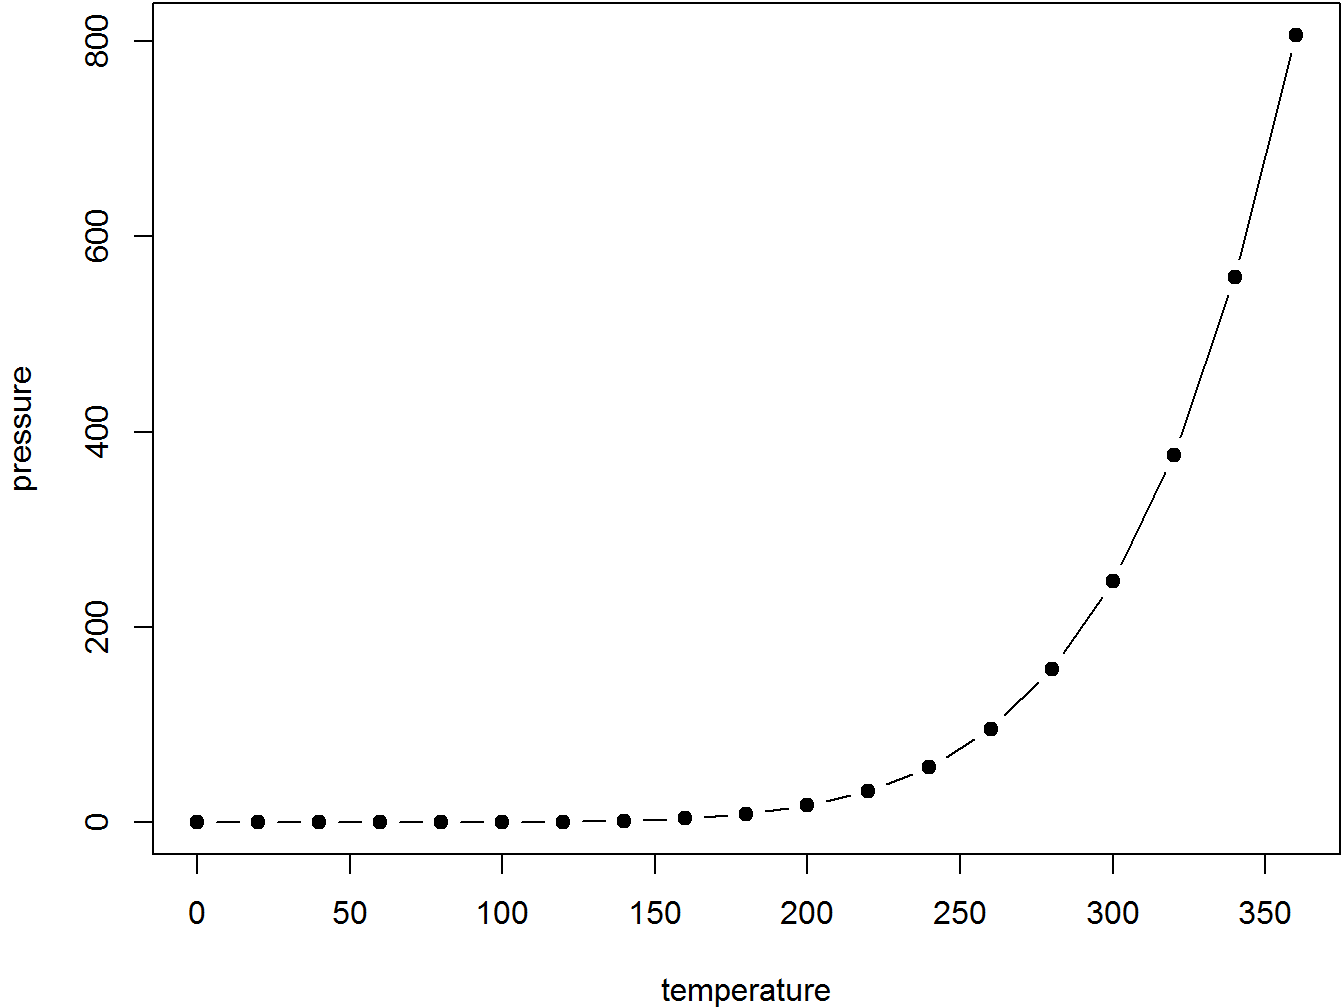
\includegraphics[width=0.8\linewidth]{code-inventory_files/figure-latex/nice-fig-1} 

}

\caption{Here is a nice figure!}\label{fig:nice-fig}
\end{figure}

Reference a figure by its code chunk label with the \texttt{fig:} prefix, e.g., see Figure \ref{fig:nice-fig}. Similarly, you can reference tables generated from \texttt{knitr::kable()}, e.g., see Table \ref{tab:nice-tab}.

\begin{Shaded}
\begin{Highlighting}[]
\NormalTok{knitr}\OperatorTok{::}\KeywordTok{kable}\NormalTok{(}
  \KeywordTok{head}\NormalTok{(iris, }\DecValTok{20}\NormalTok{), }\DataTypeTok{caption =} \StringTok{'Here is a nice table!'}\NormalTok{,}
  \DataTypeTok{booktabs =} \OtherTok{TRUE}
\NormalTok{)}
\end{Highlighting}
\end{Shaded}

\begin{table}

\caption{\label{tab:nice-tab}Here is a nice table!}
\centering
\begin{tabular}[t]{rrrrl}
\toprule
Sepal.Length & Sepal.Width & Petal.Length & Petal.Width & Species\\
\midrule
5.1 & 3.5 & 1.4 & 0.2 & setosa\\
4.9 & 3.0 & 1.4 & 0.2 & setosa\\
4.7 & 3.2 & 1.3 & 0.2 & setosa\\
4.6 & 3.1 & 1.5 & 0.2 & setosa\\
5.0 & 3.6 & 1.4 & 0.2 & setosa\\
\addlinespace
5.4 & 3.9 & 1.7 & 0.4 & setosa\\
4.6 & 3.4 & 1.4 & 0.3 & setosa\\
5.0 & 3.4 & 1.5 & 0.2 & setosa\\
4.4 & 2.9 & 1.4 & 0.2 & setosa\\
4.9 & 3.1 & 1.5 & 0.1 & setosa\\
\addlinespace
5.4 & 3.7 & 1.5 & 0.2 & setosa\\
4.8 & 3.4 & 1.6 & 0.2 & setosa\\
4.8 & 3.0 & 1.4 & 0.1 & setosa\\
4.3 & 3.0 & 1.1 & 0.1 & setosa\\
5.8 & 4.0 & 1.2 & 0.2 & setosa\\
\addlinespace
5.7 & 4.4 & 1.5 & 0.4 & setosa\\
5.4 & 3.9 & 1.3 & 0.4 & setosa\\
5.1 & 3.5 & 1.4 & 0.3 & setosa\\
5.7 & 3.8 & 1.7 & 0.3 & setosa\\
5.1 & 3.8 & 1.5 & 0.3 & setosa\\
\bottomrule
\end{tabular}
\end{table}

\hypertarget{stfrancis}{%
\chapter{St Francis}\label{stfrancis}}

This document is intended to catalog and document all of the code for St Francis as well as how to use it.

\hypertarget{project-structure-1}{%
\section{Project Structure}\label{project-structure-1}}

\hypertarget{notes-questions-1}{%
\section{Notes / Questions}\label{notes-questions-1}}

\begin{itemize}
\item
  TBA
\item
\end{itemize}

\hypertarget{r-code-1}{%
\section{\texorpdfstring{\texttt{R} Code}{R Code}}\label{r-code-1}}

\hypertarget{r-1}{%
\subsection{\texorpdfstring{\texttt{/r}}{/r}}\label{r-1}}

\hypertarget{inpatient_main.r}{%
\subsubsection{\texorpdfstring{\texttt{inpatient\_main.R}}{inpatient\_main.R}}\label{inpatient_main.r}}

\begin{itemize}
\tightlist
\item
  \texttt{setupLogging()} - Sets up the futile logger
\item
  \texttt{get\_params()} - Configuration / Initialization settings to build the St Francis dataset and model
\item
  \texttt{connect\_to\_dbs()} -
\item
  \texttt{get\_params\_from\_file()} - Loads the parameter object from an initialziation file.
\item
  \texttt{prompt\_for\_ini\_location()} - Prompt the user for the location of their initialization file. Verifies the user input that the file exists.
\item
  \texttt{load\_libraries()} -
\item
  \texttt{set\_params\_datetime()} - Function used to modify the date and time in the parameters object, used to determine the demarcation point where the data is truncated.
\item
  \texttt{set\_rds\_directory()} - Function used to set the RDS directory on the params object, including locations to X and Y dataset files.
\item
  \texttt{add\_common\_data()} -
\item
  \texttt{get\_params\_dev\_RV()} - Convenience function to get parameters for devleopment
\item
  \texttt{get\_params\_prod\_RV()} - Convenience function to get parameters to test production processing
\item
  \texttt{get\_params\_dev\_jg()} - Convenience function to get parameters to test dev processing
\item
  \texttt{get\_params\_prod\_jg()} - Convenience function to get parameters to test production processing
\end{itemize}

\hypertarget{rdao-1}{%
\subsection{\texorpdfstring{\texttt{/r/dao}}{/r/dao}}\label{rdao-1}}

\hypertarget{ahrq_dao.r}{%
\subsubsection{\texorpdfstring{\texttt{AHRQ\_dao.R}}{AHRQ\_dao.R}}\label{ahrq_dao.r}}

\begin{itemize}
\tightlist
\item
  \texttt{get\_psi\_data()} - get\_psi\_data returns patients and
\item
  \texttt{run\_get\_psi\_fun()} -
\item
  \texttt{get\_psi\_02\_enc()} -
\item
  \texttt{get\_psi\_03\_enc()} -
\item
  \texttt{get\_psi\_04\_enc()} -
\item
  \texttt{get\_psi\_05\_enc()} -
\item
  \texttt{get\_psi\_06\_enc()} -
\item
  \texttt{get\_psi\_07\_enc()} -
\item
  \texttt{get\_psi\_08\_enc()} -
\item
  \texttt{get\_psi\_09\_enc()} -
\item
  \texttt{get\_psi\_10\_enc()} -
\item
  \texttt{get\_psi\_11\_enc()} -
\item
  \texttt{get\_psi\_12\_enc()} -
\item
  \texttt{get\_psi\_13\_enc()} -
\item
  \texttt{get\_psi\_14\_enc()} -
\item
  \texttt{get\_psi\_15\_enc()} -
\item
  \texttt{get\_psi\_16\_enc()} -
\item
  \texttt{get\_psi\_17\_enc()} -
\item
  \texttt{get\_psi\_18\_enc()} -
\item
  \texttt{get\_psi\_19\_enc()} -
\item
  \texttt{get\_psi\_02\_enc\_rlx()} -
\item
  \texttt{get\_psi\_03\_enc\_rlx()} -
\item
  \texttt{get\_psi\_04\_enc\_rlx()} -
\item
  \texttt{get\_psi\_05\_enc\_rlx()} -
\item
  \texttt{get\_psi\_06\_enc\_rlx()} -
\item
  \texttt{get\_psi\_07\_enc\_rlx()} -
\item
  \texttt{get\_psi\_08\_enc\_rlx()} -
\item
  \texttt{get\_psi\_09\_enc\_rlx()} -
\item
  \texttt{get\_psi\_10\_enc\_rlx()} -
\item
  \texttt{get\_psi\_11\_enc\_rlx()} -
\item
  \texttt{get\_psi\_12\_enc\_rlx()} -
\item
  \texttt{get\_psi\_13\_enc\_rlx()} -
\item
  \texttt{get\_psi\_14\_enc\_rlx()} -
\item
  \texttt{get\_psi\_15\_enc\_rlx()} -
\item
  \texttt{get\_psi\_16\_enc\_rlx()} -
\item
  \texttt{get\_psi\_17\_enc\_rlx()} -
\item
  \texttt{get\_psi\_18\_enc\_rlx()} -
\item
  \texttt{get\_psi\_19\_enc\_rlx()} -
\end{itemize}

\hypertarget{dx_dao.r}{%
\subsubsection{\texorpdfstring{\texttt{Dx\_dao.R}}{Dx\_dao.R}}\label{dx_dao.r}}

\begin{itemize}
\tightlist
\item
  \texttt{get\_pt\_diagnosis()} -
\end{itemize}

\hypertarget{enc_dao.r}{%
\subsubsection{\texorpdfstring{\texttt{Enc\_dao.R}}{Enc\_dao.R}}\label{enc_dao.r}}

\begin{itemize}
\tightlist
\item
  \texttt{get\_arrival\_data()} - In lieie of having the ER arrival time, this determines the likely arrival time by pegging it off the first lab , chart or assessement measurement. These can be sometimes months before the encounter so it limits measuements taken to those within 72 hours of admit date.
\item
  \texttt{get\_historical\_encounters()} -
\item
  \texttt{get\_discharge\_disposition()} - Get the D/C disposition and cleans up the discharge setting by trianfulating with referral placements
\item
  \texttt{get\_discharge\_disposition2()} - Another getter function to get a patient discharge disposition. This merges with the discharge decords and casts into wide format.
\item
  \texttt{get\_pts\_last\_unit()} -
\item
  \texttt{get\_admission\_file()} -
\item
  \texttt{get\_ecin\_admission\_file()} -
\item
  \texttt{get\_star\_admission\_file()} -
\item
  \texttt{getCrossSectionalDataset()} - Gets cross sectional dataset for every admission. The sample is defined by the parameters of the function, which indicate which sample to discard. The defaults are set to what you would want in a readmission analysis (not LOS).
\item
  \texttt{get\_encounter\_LOS\_data()} - Get all patient encounters LOS related metrics.
\item
  \texttt{get\_readmission\_data()} -
\item
  \texttt{get\_return\_ed\_visits()} - get\_return\_ed\_visits gets stays that result in a ed visit 72hrs or less after discharge
\item
  \texttt{get\_ed\_visit\_data()} - get\_ed\_visit\_data Returns ED visit info for star schema - including visit and los (minutes)
\item
  \texttt{develop\_dc\_referral\_xwalk()} - INCOMPLETE -- IS THIS USED??? Maybe to clean up the acuity target? IF NOT DEPRECATE
\item
  \texttt{get\_all\_valid\_pat\_types()} - get\_all\_valid\_pat\_types using pat\_type\_decode, returns all potential pat\_types for analysis
\item
  \texttt{get\_encounter\_date\_data()} - get\_encounter\_date\_data get admit and discharge times of all encounters
\item
  \texttt{get\_pt\_financial\_class()} - get\_pt\_financial\_class gets financial class of all patients (xmatches on mapping xls)
\item
  \texttt{get\_pt\_demographics()} -
\item
  \texttt{make\_pat\_type\_sql()} - make\_pat\_type\_sql produces where clause from list of patient types passed in
\end{itemize}

\hypertarget{lab_dao.r}{%
\subsubsection{\texorpdfstring{\texttt{Lab\_dao.R}}{Lab\_dao.R}}\label{lab_dao.r}}

\begin{itemize}
\item
\end{itemize}

\hypertarget{tx_dao.r}{%
\subsubsection{\texorpdfstring{\texttt{Tx\_dao.R}}{Tx\_dao.R}}\label{tx_dao.r}}

\begin{itemize}
\tightlist
\item
  \texttt{get\_abx\_prophylaxis\_txs()} -
\item
  \texttt{get\_pt\_procedures()} -
\item
  \texttt{get\_ccs\_procedures()} -
\item
  \texttt{get\_mech\_vent\_data()} -
\item
  \texttt{get\_catheter\_order\_groupings()} - Reads in a decode file that distinguishes which orders are CAUTI or CLABSI related.
\item
  \texttt{get\_cauti\_related\_orders()} -
\item
  \texttt{get\_cauti\_related\_dc\_orders()} -
\item
  \texttt{get\_clabsi\_related\_orders()} -
\item
  \texttt{get\_clabsi\_related\_dc\_orders()} -
\item
  \texttt{get\_orders\_data\_by\_name()} -
\item
  \texttt{get\_prc\_hx\_by\_name\_data()} - get\_prc\_hx\_by\_name\_data returns patients with historical prc's entered by name or icd code (finds encounters of a patient with a prc in a previous encounter)
\end{itemize}

\hypertarget{vital_dao.r}{%
\subsubsection{\texorpdfstring{\texttt{Vital\_dao.R}}{Vital\_dao.R}}\label{vital_dao.r}}

\begin{itemize}
\tightlist
\item
  \texttt{get\_mckesson\_temperature\_data()} - get\_temperature\_data returns temperature data from CHARTS with temp\_abnormal flag \#' \citet{param} params
\item
  \texttt{get\_mckesson\_blood\_pressure\_data()} -
\item
  \texttt{get\_mckesson\_map\_data()} -
\item
  \texttt{get\_mckesson\_pulse\_data()} -
\item
  \texttt{get\_mckesson\_respiration\_rate\_data()} -
\item
  \texttt{get\_mckesson\_chart\_data()} -
\end{itemize}

\hypertarget{rcommon}{%
\subsection{\texorpdfstring{\texttt{/r/common}}{/r/common}}\label{rcommon}}

\hypertarget{build_sf_models.r}{%
\subsubsection{\texorpdfstring{\texttt{build\_sf\_models.R}}{build\_sf\_models.R}}\label{build_sf_models.r}}

\begin{itemize}
\tightlist
\item
  \texttt{build\_sf\_models()} - Build's all of the longitudinal models for St Francis
\item
  \texttt{build\_sf\_windowed\_models()} -
\item
  \texttt{get\_blocked\_variables()} - Variables blacklisted from modelling
\item
  \texttt{build\_sf\_day\_models()} -
\item
  \texttt{slice\_dataset\_by\_interval()} - Split the X, XRF, and Y datasets up by day, saves individual files to the RDS directory
\item
  \texttt{promote\_sf\_models()} -
\end{itemize}

\hypertarget{data_converters.r}{%
\subsubsection{\texorpdfstring{\texttt{data\_converters.R}}{data\_converters.R}}\label{data_converters.r}}

\begin{itemize}
\tightlist
\item
  \texttt{convertToDate()} - Function used to convert the date format in the ancillairy file
\item
  \texttt{dateToPOSIXct()} - Converts a Data to POSIXct without screwing up and offesetting the time to EST.
\end{itemize}

\hypertarget{database_access.r}{%
\subsubsection{\texorpdfstring{\texttt{database\_access.R}}{database\_access.R}}\label{database_access.r}}

\begin{itemize}
\tightlist
\item
  \texttt{save\_results\_to\_db2()} - Save the results of main\_processing to the inpatient\_results\_table
\item
  \texttt{get\_next\_result\_id()} -
\item
  \texttt{get\_next\_reason\_id()} -
\item
  \texttt{propogate\_discharges()} - Checks if a model has already been run for the specified date.
\item
  \texttt{process\_timeline\_data()} -
\item
  \texttt{update\_pt\_location()} - Updates the patient room, unit, and bed location to the latest.
\item
  \texttt{check\_if\_data\_already\_present()} - Checks if a model has already been run for the specified date.
\item
  \texttt{delete\_data\_as\_of\_datetime()} - Deletes records fromthe model results table for the specified date
\end{itemize}

\hypertarget{dedupe.r}{%
\subsubsection{\texorpdfstring{\texttt{dedupe.R}}{dedupe.R}}\label{dedupe.r}}

\begin{itemize}
\tightlist
\item
  \texttt{train\_pt\_deduper()} -
\item
  \texttt{get\_pt\_pairs()} -
\item
  \texttt{run\_pt\_deduper()} -
\item
  \texttt{dedupe\_mrn()} -
\end{itemize}

\hypertarget{load_sf.r}{%
\subsubsection{\texorpdfstring{\texttt{load\_sf.R}}{load\_sf.R}}\label{load_sf.r}}

\begin{itemize}
\tightlist
\item
  \texttt{buildFullDb()} - Load all of the raw data (full csv dumps) into the St Francis database.
\item
  \texttt{loadPlacementData()} -
\item
  \texttt{loadAssessmentData()} -
\item
  \texttt{loadRxData()} -
\item
  \texttt{loadChartData()} - Reads in the chart data CSV files, combines them, types the data, and saves them to the SQL Server database.
\item
  \texttt{loadLabData()} - Reads in the lab data CSV files, combines them, types the data, and saves them to the SQL Server database.
\item
  \texttt{loadAdmissionAssessmentData()} - Reads in the lab data CSV files, combines them, types the data, and saves them to the SQL Server database.
\item
  \texttt{loadDischargeAssessmentData()} - Reads in the discharge assessment data CSV files, combines them, types the data, and saves them to the SQL Server database.
\item
  \texttt{loadEncounterData()} - Reads in the encounter data CSV files, combines them, types the data, and saves them to the SQL Server database.
\item
  \texttt{loadOrderData()} -
\item
  \texttt{merge\_dbs()} -
\item
  \texttt{merge\_table()} -
\item
  \texttt{loadFlowSheetData()} -
\item
  \texttt{loadRISData()} - loadRISData loads RIS data from txt file and saves to DB set latest\_only=T if ``replaying'' PROD feed files need to be named correctly (date needs to be in there in a format such that max() will work) for this to work TODO append?
\item
  \texttt{loadCulturesData()} - loadCulturesData loads HCI cultures data from txt file and saves to DB TODO append?
\item
  \texttt{loadNewOrderData()} - loadNewOrderData loads new Order data (addl fields)
\item
  \texttt{extract\_zip\_data()} - extract\_zip\_data extracts file(s) out of zips - used to pull data from historical daily zips fed by SF
\item
  \texttt{loadMDMasterData()} - loadMDMasterData loads new MD Master data
\item
  \texttt{loadMedhostData()} - loadMDMasterData loads new Medhost data
\item
  \texttt{load\_SurgicalExtract\_data()} - load\_SurgicalExtract\_data loads CPM surgical extract data
\item
  \texttt{load\_allergy\_data()} -
\item
  \texttt{loadMedOrdersData()} -
\item
  \texttt{loadMedAdminData()} -
\end{itemize}

\hypertarget{load_supplemental_data.r}{%
\subsubsection{\texorpdfstring{\texttt{load\_supplemental\_data.R}}{load\_supplemental\_data.R}}\label{load_supplemental_data.r}}

\begin{itemize}
\tightlist
\item
  \texttt{loadSupplementalData()} - Loads all of the code/decode and reference data in SVN that is used preprocess the data
\item
  \texttt{loadCMSDRG()} - load the medicaire drg decodes table for 2014
\item
  \texttt{loadDRGs2del()} - load the DRG's to be eliminiated
\item
  \texttt{loadInsPlans()} - load the insurance plans
\item
  \texttt{loadInsPlanGroups()} - load the plan groupings from SF
\item
  \texttt{loadTricareDRGs()} - load the tricare drgs
\item
  \texttt{loadDRGPenalties()} - load the file indicating which DRG's are subject to penalty
\item
  \texttt{loadPatientTypes()} - load the file the provide a decode for patient types
\item
  \texttt{loadDischargeCodes()} - load the discharge codes and groups
\item
  \texttt{loadNDC()} - National drug database
\item
  \texttt{loadDRGv24()} - v24 DRG grouper data, infer GMLOS form AMLOS
\end{itemize}

\hypertarget{run_common.r}{%
\subsubsection{\texorpdfstring{\texttt{run\_common.R}}{run\_common.R}}\label{run_common.r}}

\begin{itemize}
\tightlist
\item
  \texttt{get\_x\_controller()} -
\item
  \texttt{list\_missing\_build\_x\_rds()} - List out missing build x rds files in the RDS directory. Reconciles against the x\_controller to determine difference so that you can easily reprocess a subset of the missing build\_x functions by using the output of this as a parameter in the build\_model function
\item
  \texttt{preprocess\_data()} - Preprocesses the raw data into a target and predictor variables dataset. The predictor variables that are preprocess are defiend by the ``x\_controller''. This is a list of functions that the preprocessor will run through. These functions build a portion of the X dataset.
\item
  \texttt{cbind\_build\_x()} - Merges an and array of build\_x\_* functions into the final longitudinal X dataset.
\item
  \texttt{build\_x\_from\_array()} - TO BE DEPRECATED
\item
  \texttt{build\_x\_from\_rds()} -
\item
  \texttt{which\_x\_rds\_has()} - Traces through the RDS files to fine the source for a particular variable
\item
  \texttt{verify\_and\_prep()} -
\item
  \texttt{standardize\_build\_data()} - Runs the X data preprocessing function passed to it with exception handling.
\item
  \texttt{get\_emr\_last\_update\_time()} - Estimates when the EMR was last updated by looking for the latest labs and orders
\end{itemize}

\hypertarget{run_dev.r}{%
\subsubsection{\texorpdfstring{\texttt{run\_dev.R}}{run\_dev.R}}\label{run_dev.r}}

\begin{itemize}
\tightlist
\item
  \texttt{get\_dev\_end\_date()} -
\item
  \texttt{build\_dataset()} -
\end{itemize}

\hypertarget{run_prod.r}{%
\subsubsection{\texorpdfstring{\texttt{run\_prod.R}}{run\_prod.R}}\label{run_prod.r}}

\begin{itemize}
\tightlist
\item
  \texttt{try\_main\_processing()} - main\_processing function surrounded in a tryCatch block for better error logging.
\item
  \texttt{main\_processing()} - Main production processing routine the preprocesses the raw data, checks for data errors, run the data through the models, producing scores and predictions. Then it runs the explainer and the rule engine. Finally, saving everyting to the production web database.
\item
  \texttt{main\_update()} -
\item
  \texttt{conform\_data()} - Adds any required variables the may have not been computed, usually as a result of data-driven variables. Also subsets to only those variables that are required for either model processing or rule processing.
\item
  \texttt{add\_last\_scores()} - Get the last predictions \& join them to the predictions table Note: assume that the current scores are not in the DB - trust that these are previous Note: side effect will be that a double entry of a score will yeild an unchanged indicator
\item
  \texttt{get\_model\_files()} - Get's a list of files where all the models are
\item
  \texttt{process\_models()} - Processes the xrf dataset through all of the models
\item
  \texttt{transform\_predictions()} -
\item
  \texttt{process\_expert\_models()} -
\item
  \texttt{process\_scores()} - Process the predictions into scores for all models by using the scoring cross reference established in development.
\item
  \texttt{get\_reason\_files()} - Get's all of the bin files used by the explainer
\item
  \texttt{process\_reasons()} - Use the predictions to develop explain reasons for why high or low
\item
  \texttt{process\_dates()} - Processes the predictions to convert into absolute dates w/ confidence intervals for days remaining and GMLOS cutoff date
\item
  \texttt{process\_confidence\_intervals()} - Determines the confidence interval for the predictions
\item
  \texttt{ci\_lookup()} - Determines the confidence interval for an individual prediction
\item
  \texttt{get\_probable\_dc\_destinations()} -
\item
  \texttt{get\_probable\_dc\_destinations()} -
\item
  \texttt{get\_top()} -
\item
  \texttt{scale\_predictions()} -
\item
  \texttt{propogate\_obs\_patients()} - refresh\_obs\_patients refreshes observation\_model\_results table of consumption by website
\item
  \texttt{create\_model\_action\_relation\_tables()} - Mobile App X-Ref table generator
\end{itemize}

\hypertarget{setup_prod.r-1}{%
\subsubsection{\texorpdfstring{\texttt{setup\_prod.R}}{setup\_prod.R}}\label{setup_prod.r-1}}

\begin{itemize}
\tightlist
\item
  \texttt{setup\_prod()} - Set's up the production architecture, including profiling for data validation, explain reasons, merging XRF datasets across model runs, preparing the ``makeRF'' context, confidnce intervals, payor grid, and provider grids.
\item
  \texttt{prepare\_validation\_profile()} - Prepares the validation profile that is used in produciton for data validation
\item
  \texttt{prepare\_scoring\_xref()} - Develops the scoring cross reference in development for use in production.
\item
  \texttt{get\_all\_predictions\_from\_rf()} - Gets all of the predictions attached to the random forest object (traiing and test -- if it exists).
\item
  \texttt{run\_all\_predictions()} - Gets all the predictions by running the xrf dataset through all of the models
\item
  \texttt{prepare\_explainer()} -
\item
  \texttt{prepare\_makeRFContext()} - Reads in the XRF and saves out the context data (naVals, vLevels, outlierBounds, colClasses)
\item
  \texttt{replay\_prod()} - Replays productoin processing over a time window specified by the number of days from and to today.
\item
  \texttt{merge\_reasons()} - Merges reasons between two reason files
\item
  \texttt{prepare\_confidence\_intervals()} -
\item
  \texttt{setup\_rx\_xref()} -
\end{itemize}

\hypertarget{shared_functions.r}{%
\subsubsection{\texorpdfstring{\texttt{shared\_functions.R}}{shared\_functions.R}}\label{shared_functions.r}}

\begin{itemize}
\tightlist
\item
  \texttt{loadDatabase()} - load the entire st francis database into R objects
\end{itemize}

\hypertarget{utils.r}{%
\subsubsection{\texorpdfstring{\texttt{utils.R}}{utils.R}}\label{utils.r}}

\begin{itemize}
\item
\end{itemize}

\hypertarget{validate_prod.r}{%
\subsubsection{\texorpdfstring{\texttt{validate\_prod.R}}{validate\_prod.R}}\label{validate_prod.r}}

\begin{itemize}
\tightlist
\item
  \texttt{validate\_data()} - Check for data shift errrors.
\item
  \texttt{validate\_raw\_db()} - Runs a new of validation test on the raw database (StFrancis)
\item
  \texttt{run\_validation\_rule()} - Runs a validation rule
\item
  \texttt{validate\_ecin\_admissions()} - Validates there are some dischages for params\$as\_of\_date
\item
  \texttt{validate\_ecin\_admission\_analysis()} - Validates there are some dischages for params\$as\_of\_date
\item
  \texttt{validate\_ecin\_assessments()} - Validates there are some assessments for params\$as\_of\_date
\item
  \texttt{validate\_ecin\_payor\_comm()} - Validates there are some payor communications exists for params\$as\_of\_date
\item
  \texttt{validate\_ecin\_referrals()} - Validates there are some ecin referrals for params\$as\_of\_date
\item
  \texttt{validate\_ecin\_referrals\_delivered()} - Validates there are some ecin referrals delivered for params\$as\_of\_date
\item
  \texttt{validate\_hci\_adm\_assessment()} - Validates there are some admissions assessements for params\$as\_of\_date
\item
  \texttt{validate\_hci\_charts()} - Validates there are charts for params\$as\_of\_date
\item
  \texttt{validate\_disch\_assessment()} - Validates there are charts for params\$as\_of\_date
\item
  \texttt{validate\_hci\_flowsheet()} - Validates there are flowsheets for params\$as\_of\_date
\item
  \texttt{validate\_hci\_labs()} - Validates there are labs for params\$as\_of\_date
\item
  \texttt{validate\_star\_encounters()} - Validates there are labs for params\$as\_of\_date
\item
  \texttt{validate\_hci\_orders()} - Validates there are labs for params\$as\_of\_date
\item
  \texttt{validate\_hci\_medadmin()} - Validates there are rx rders for params\$as\_of\_date
\item
  \texttt{validate\_hci\_medorders()} -
\item
  \texttt{validate\_hci\_ris()} - Validates there are rx rders for params\$as\_of\_date
\item
  \texttt{validate\_hci\_medhost()} - Validates there are rx rders for params\$as\_of\_date
\item
  \texttt{validate\_hci\_anc()} - Validates there are rx rders for params\$as\_of\_date
\item
  \texttt{validate\_hci\_cpm()} - Validates there are rx rders for params\$as\_of\_date
\item
  \texttt{validate\_emr\_recency()} -
\item
  \texttt{prevalidate\_inbound\_files()} - Validates inbound raw , delimitted data files for structural integrity (correct \# of delimiters,etc.)
\end{itemize}

\hypertarget{rrules-1}{%
\subsection{\texorpdfstring{\texttt{/r/rules}}{/r/rules}}\label{rrules-1}}

\hypertarget{build_rules_inputs.r}{%
\subsubsection{\texorpdfstring{\texttt{build\_rules\_inputs.R}}{build\_rules\_inputs.R}}\label{build_rules_inputs.r}}

\begin{itemize}
\tightlist
\item
  \texttt{get\_rule\_inputs()} - Pull all the fields required from data.x for running the rules
\item
  \texttt{build\_rule\_inputs\_pass\_1()} - First stage of generating the inputs to the rules by mapping both the data.x fields and contents to the intended decision keys. ``1st pass'' fields are those that are upstream from the model and can be derived exclusively off of the X dataset.
\item
  \texttt{build\_rule\_inputs\_pass\_2()} - Second stage of generating the inputs to the rules by mapping both the data.x fields and contents to the intended decision keys. ``2nd pass'' fields are those that are downstream from the model predictions.
\item
  \texttt{get\_val\_counts()} - Save out the value tally csv for each of the columns
\item
  \texttt{get\_val\_counts2()} - Save out the value tally csv for each of the columns
\item
  \texttt{get\_rule\_counts()} - Retrieve all the rules and actions from the DB, processes and saves counts.
\end{itemize}

\hypertarget{case_mgr_rule_defs.r}{%
\subsubsection{\texorpdfstring{\texttt{case\_mgr\_rule\_defs.R}}{case\_mgr\_rule\_defs.R}}\label{case_mgr_rule_defs.r}}

\begin{itemize}
\tightlist
\item
  \texttt{rule\_1AB\_complete\_dc\_planning\_assmt()} -
\item
  \texttt{rule\_2\_identify\_dc\_setting()} -
\item
  \texttt{rule\_3\_escalate\_dc\_setting()} -
\item
  \texttt{rule\_4A\_post\_acute\_auth()} -
\item
  \texttt{rule\_4B\_payer\_contraints()} -
\item
  \texttt{rule\_5\_alternate\_referral()} -
\item
  \texttt{rule\_7a\_home\_02()} -
\item
  \texttt{rule\_7b\_process\_referral\_phys\_therapy()} -
\item
  \texttt{rule\_7b\_all\_schedule\_phys\_therapy()} -
\item
  \texttt{rule\_7c\_speech\_therapy()} -
\item
  \texttt{rule\_7c2\_speech\_therapy()} -
\item
  \texttt{rule\_7d\_wound\_care()} - TODO deprecate for rule 27???? rule 27 to change verbage
\item
  \texttt{rule\_8\_higher\_level\_post\_acute()} -
\item
  \texttt{rule\_9\_lower\_level\_post\_acute()} -
\item
  \texttt{rule\_11BC\_follow\_up\_post\_dc()} -
\item
  \texttt{rule\_12\_refer\_to\_CDI()} -
\item
  \texttt{rule\_13\_has\_PCP()} -
\item
  \texttt{rule\_14\_homeless()} -
\item
  \texttt{rule\_15\_LTAC()} -
\item
  \texttt{rule\_17\_review\_dc\_assmt()} -
\item
  \texttt{rule\_18\_review\_dc\_assmt()} -
\item
  \texttt{rule\_19\_review\_dc\_assmt()} -
\item
  \texttt{rule\_20ABC\_complete\_dc\_process()} -
\item
  \texttt{rule\_21\_min\_criteria\_ARHB()} -
\item
  \texttt{rule\_21b\_min\_criteria\_SNF()} -
\item
  \texttt{rule\_21c\_min\_criteria\_HH()} -
\item
  \texttt{rule\_22\_post\_acute\_grid()} -
\item
  \texttt{rule\_23\_diabetic\_test()} -
\item
  \texttt{rule\_24\_diabetic\_education()} -
\item
  \texttt{rule\_25\_letter\_of\_med\_necessity()} -
\item
  \texttt{rule\_26\_certification\_letter\_day17()} -
\item
  \texttt{rule\_26\_certification\_letter\_day37()} -
\item
  \texttt{rule\_26\_certification\_letter\_day57()} -
\item
  \texttt{rule\_27\_braden\_score()} -
\item
  \texttt{rule\_28\_nutrition()} -
\item
  \texttt{rule\_29\_gmlos\_exceeded()} -
\item
  \texttt{rule\_30\_gmlos\_exceeded\_a\_lot()} -
\item
  \texttt{rule\_31\_is\_readmission()} -
\end{itemize}

\hypertarget{infectious_rule_defs.r}{%
\subsubsection{\texorpdfstring{\texttt{infectious\_rule\_defs.R}}{infectious\_rule\_defs.R}}\label{infectious_rule_defs.r}}

\begin{itemize}
\tightlist
\item
  \texttt{rule\_sepsis\_mono\_therapy()} -
\item
  \texttt{rule\_sepsis\_combination\_therapy\_septic\_shock()} -
\item
  \texttt{rule\_sepsis\_antibiotic\_biogram()} -
\item
  \texttt{rule\_antibiotic\_organism()} -
\item
  \texttt{rule\_antibiotic\_gram\_stain()} -
\item
  \texttt{rule\_antibiotic\_culture\_sensitivities()} -
\end{itemize}

\hypertarget{pne_rule_defs.r}{%
\subsubsection{\texorpdfstring{\texttt{pne\_rule\_defs.R}}{pne\_rule\_defs.R}}\label{pne_rule_defs.r}}

\begin{itemize}
\tightlist
\item
  \texttt{may\_be\_treated\_for\_pne()} -
\item
  \texttt{is\_suspected\_pne()} -
\item
  \texttt{rule\_pne\_is\_being\_treated()} -
\end{itemize}

\hypertarget{run_rules.r}{%
\subsubsection{\texorpdfstring{\texttt{run\_rules.R}}{run\_rules.R}}\label{run_rules.r}}

\begin{itemize}
\tightlist
\item
  \texttt{process\_rules()} - Runs the data through the rule engine, saving to DB
\item
  \texttt{get\_rule\_controller()} -
\item
  \texttt{run\_all\_rules()} - runs all the rules defined by the rule controller
\item
  \texttt{process\_actions()} - Compares the output of run\_all\_rules() with existing actions in the DB - inserts or updates as necessary
\item
  \texttt{get\_required\_rule\_output()} -
\item
  \texttt{process\_rule\_sequence\_table()} -
\item
  \texttt{auto\_close\_actions()} -
\end{itemize}

\hypertarget{sepsis_rule_defs.r}{%
\subsubsection{\texorpdfstring{\texttt{sepsis\_rule\_defs.R}}{sepsis\_rule\_defs.R}}\label{sepsis_rule_defs.r}}

\begin{itemize}
\tightlist
\item
  \texttt{has\_exceeded\_sepsis\_dx\_thresholds()} -
\item
  \texttt{has\_exceeded\_sepsis\_dx\_t\_thresholds()} -
\item
  \texttt{may\_be\_treated\_for\_sepsis()} -
\item
  \texttt{may\_be\_treated\_for\_severe\_sepsis()} -
\item
  \texttt{is\_being\_treated\_for\_sepsis()} -
\item
  \texttt{is\_being\_treated\_for\_severe\_sepsis()} -
\item
  \texttt{is\_suspected\_sepsis()} -
\item
  \texttt{rule\_sepsis\_omega3()} -
\item
  \texttt{rule\_sepsis\_procalcitonin()} -
\item
  \texttt{rule\_sepsis\_antithrombin()} -
\item
  \texttt{rule\_sepsis\_iv\_selenium()} -
\item
  \texttt{rule\_sepsis\_hydroxyethyl\_starches()} -
\item
  \texttt{rule\_sepsis\_dopamine()} -
\item
  \texttt{rule\_sepsis\_pac\_ards()} -
\item
  \texttt{rule\_sepsis\_erythropoietin()} -
\item
  \texttt{rule\_sepsis\_prone\_position()} -
\item
  \texttt{rule\_sepsis\_iv\_immunoglobulins()} -
\item
  \texttt{rule\_sepsis\_rbc\_transfusion()} -
\item
  \texttt{rule\_sepsis\_hob\_angle()} -
\item
  \texttt{rule\_sepsis\_ufh\_lmwh\_vte()} -
\item
  \texttt{rule\_sepsis\_lmwh\_over\_ufh()} -
\item
  \texttt{rule\_sepsis\_tpn()} -
\item
  \texttt{rule\_sepsis\_pud()} -
\item
  \texttt{rule\_sepsis\_3hb\_lactate()} -
\item
  \texttt{rule\_sepsis\_3hb\_recheck\_lactate()} -
\item
  \texttt{rule\_sepsis\_3hb\_blood\_culture()} -
\item
  \texttt{rule\_sepsis\_3hb\_broad\_spectrum\_abx()} -
\item
  \texttt{rule\_sepsis\_3hb\_crystalloids()} -
\item
  \texttt{rule\_sepsis\_order\_bp()} -
\item
  \texttt{rule\_sepsis\_suspected\_lactates()} -
\item
  \texttt{rule\_sepsis\_suspected\_blood\_cultures()} -
\item
  \texttt{rule\_sepsis\_is\_being\_treated()} -
\item
  \texttt{rule\_severe\_sepsis\_is\_being\_treated()} -
\item
  \texttt{rule\_sepsis\_order\_blood\_culture()} -
\item
  \texttt{rule\_sepsis\_order\_lactates()} -
\end{itemize}

\hypertarget{uti_rule_defs.r}{%
\subsubsection{\texorpdfstring{\texttt{uti\_rule\_defs.R}}{uti\_rule\_defs.R}}\label{uti_rule_defs.r}}

\begin{itemize}
\tightlist
\item
  \texttt{may\_be\_treated\_for\_uti()} -
\item
  \texttt{is\_suspected\_uti()} -
\item
  \texttt{rule\_uti\_is\_being\_treated()} -
\end{itemize}

\hypertarget{rbuild_dataset}{%
\subsection{\texorpdfstring{\texttt{/r/build\_dataset}}{/r/build\_dataset}}\label{rbuild_dataset}}

\hypertarget{build_x_dataset_actions.r}{%
\subsubsection{\texorpdfstring{\texttt{build\_x\_dataset\_actions.R}}{build\_x\_dataset\_actions.R}}\label{build_x_dataset_actions.r}}

\begin{itemize}
\item
\end{itemize}

\hypertarget{build_x_dataset_admission.r}{%
\subsubsection{\texorpdfstring{\texttt{build\_x\_dataset\_admission.R}}{build\_x\_dataset\_admission.R}}\label{build_x_dataset_admission.r}}

\begin{itemize}
\tightlist
\item
  \texttt{build\_x\_adm\_assmt()} -
\end{itemize}

\hypertarget{build_x_dataset_anci.r}{%
\subsubsection{\texorpdfstring{\texttt{build\_x\_dataset\_ANCI.R}}{build\_x\_dataset\_ANCI.R}}\label{build_x_dataset_anci.r}}

\begin{itemize}
\item
\end{itemize}

\hypertarget{build_x_dataset_charts.r}{%
\subsubsection{\texorpdfstring{\texttt{build\_x\_dataset\_charts.R}}{build\_x\_dataset\_charts.R}}\label{build_x_dataset_charts.r}}

\begin{itemize}
\tightlist
\item
  \texttt{make\_chart\_value\_tables\_xls()} -
\end{itemize}

\hypertarget{build_x_dataset_cultures.r}{%
\subsubsection{\texorpdfstring{\texttt{build\_x\_dataset\_cultures.R}}{build\_x\_dataset\_cultures.R}}\label{build_x_dataset_cultures.r}}

\begin{itemize}
\tightlist
\item
  \texttt{build\_x\_cultures()} - build\_x\_cultures produces cultures ind variables for inpatient models
\item
  \texttt{monthly\_cultures\_counts()} -
\item
  \texttt{sortUniqueCollapse()} -
\end{itemize}

\hypertarget{build_x_dataset_discharge.r}{%
\subsubsection{\texorpdfstring{\texttt{build\_x\_dataset\_discharge.R}}{build\_x\_dataset\_discharge.R}}\label{build_x_dataset_discharge.r}}

\begin{itemize}
\tightlist
\item
  \texttt{build\_x\_disch\_assmt()} -
\end{itemize}

\hypertarget{build_x_dataset_dx.r}{%
\subsubsection{\texorpdfstring{\texttt{build\_x\_dataset\_dx.R}}{build\_x\_dataset\_dx.R}}\label{build_x_dataset_dx.r}}

\begin{itemize}
\tightlist
\item
  \texttt{build\_x\_dx()} -
\item
  \texttt{get\_dx\_ccs\_comorbity\_data()} -
\end{itemize}

\hypertarget{build_x_dataset_ecin.r}{%
\subsubsection{\texorpdfstring{\texttt{build\_x\_dataset\_ECIN.R}}{build\_x\_dataset\_ECIN.R}}\label{build_x_dataset_ecin.r}}

\begin{itemize}
\tightlist
\item
  \texttt{reshape\_referrals()} - General function to reshape referral data by different dates (post date, first yes, etc.)
\item
  \texttt{build\_x\_referrals()} - *** REFERRALS *** Determine the historical referrals
\item
  \texttt{build\_x\_assessments()} - *** ASSESSMENTS ***
\item
  \texttt{build\_x\_assessment\_notes()} - *** Assessment Notes ***
\item
  \texttt{build\_x\_cm\_notes()} - *** CM NOTES ***
\item
  \texttt{daysSince()} -
\end{itemize}

\hypertarget{build_x_dataset_encounters.r}{%
\subsubsection{\texorpdfstring{\texttt{build\_x\_dataset\_encounters.R}}{build\_x\_dataset\_encounters.R}}\label{build_x_dataset_encounters.r}}

\begin{itemize}
\tightlist
\item
  \texttt{build\_x\_encounters()} -
\end{itemize}

\hypertarget{build_x_dataset_flowsheet.r}{%
\subsubsection{\texorpdfstring{\texttt{build\_x\_dataset\_flowsheet.R}}{build\_x\_dataset\_flowsheet.R}}\label{build_x_dataset_flowsheet.r}}

\begin{itemize}
\tightlist
\item
  \texttt{build\_x\_flowsheets()} -
\item
  \texttt{build\_x\_therapy\_time()} -
\item
  \texttt{process\_fs\_metrics()} - TO BE DEPRECATED
\end{itemize}

\hypertarget{build_x_dataset_hac.r}{%
\subsubsection{\texorpdfstring{\texttt{build\_x\_dataset\_hac.R}}{build\_x\_dataset\_hac.R}}\label{build_x_dataset_hac.r}}

\begin{itemize}
\tightlist
\item
  \texttt{build\_x\_hac()} - build\_x\_hac produces hospital acquired conditions \& cdiff ind variables for inpatient models
\item
  \texttt{get\_hac\_codes()} -
\item
  \texttt{get\_hac\_reqs()} -
\item
  \texttt{get\_pt\_cleaned\_dx()} -
\item
  \texttt{get\_pt\_morbid\_obese()} -
\item
  \texttt{get\_pt\_hac()} -
\item
  \texttt{get\_pt\_hac\_cast()} - wide version of hac patient list
\item
  \texttt{get\_cdiff\_data()} -
\end{itemize}

\hypertarget{build_x_dataset_hed.r}{%
\subsubsection{\texorpdfstring{\texttt{build\_x\_dataset\_HED.R}}{build\_x\_dataset\_HED.R}}\label{build_x_dataset_hed.r}}

\begin{itemize}
\item
\end{itemize}

\hypertarget{build_x_dataset_location.r}{%
\subsubsection{\texorpdfstring{\texttt{build\_x\_dataset\_location.R}}{build\_x\_dataset\_location.R}}\label{build_x_dataset_location.r}}

\begin{itemize}
\tightlist
\item
  \texttt{build\_x\_location()} - Patient unit indicators Develop's indicators based on the patients unit, including things such as how many units (transfers) they have had, the unit's metrics (such as case mix, gmlos, etc.).
\item
  \texttt{get\_unit\_metrics()} - Gets the predominant MDC, DRG For a unit over the time period specified by sf\_y specifi
\item
  \texttt{get\_pt\_unit\_timeline()} - Returns the date from and to a patient was on a unit, along with other statistics, including \# of hrs, ICU hrs.
\end{itemize}

\hypertarget{build_x_dataset_medrec.r}{%
\subsubsection{\texorpdfstring{\texttt{build\_x\_dataset\_medrec.R}}{build\_x\_dataset\_medrec.R}}\label{build_x_dataset_medrec.r}}

\begin{itemize}
\item
\end{itemize}

\hypertarget{build_x_dataset_orders.r}{%
\subsubsection{\texorpdfstring{\texttt{build\_x\_dataset\_orders.R}}{build\_x\_dataset\_orders.R}}\label{build_x_dataset_orders.r}}

\begin{itemize}
\tightlist
\item
  \texttt{build\_x\_orders()} -
\end{itemize}

\hypertarget{build_x_dataset_patient.r}{%
\subsubsection{\texorpdfstring{\texttt{build\_x\_dataset\_patient.R}}{build\_x\_dataset\_patient.R}}\label{build_x_dataset_patient.r}}

\begin{itemize}
\item
\end{itemize}

\hypertarget{build_x_dataset_payor.r}{%
\subsubsection{\texorpdfstring{\texttt{build\_x\_dataset\_payor.R}}{build\_x\_dataset\_payor.R}}\label{build_x_dataset_payor.r}}

\begin{itemize}
\tightlist
\item
  \texttt{build\_x\_payor()} -
\item
  \texttt{build\_x\_payor\_grid()} -
\item
  \texttt{prepare\_payor\_grid()} -
\end{itemize}

\hypertarget{build_x_dataset_physician.r}{%
\subsubsection{\texorpdfstring{\texttt{build\_x\_dataset\_physician.R}}{build\_x\_dataset\_physician.R}}\label{build_x_dataset_physician.r}}

\begin{itemize}
\tightlist
\item
  \texttt{get\_pt\_md\_xref()} - Gets a cross reference data table between the patient, admitting MD, attending MD, and PCP MD.
\item
  \texttt{read\_physician\_specialty\_file()} - Gets the mainframe like physician specialty text file (from file)
\item
  \texttt{parse\_physician\_specialty\_file()} - Parses the mainframe like physician specialty file from get\_physician\_speciality\_file()
\item
  \texttt{load\_physician\_specialty()} - Gets, parses, and saves to database the mainframe like physician specialty file
\end{itemize}

\hypertarget{build_x_dataset_post_acute.r}{%
\subsubsection{\texorpdfstring{\texttt{build\_x\_dataset\_post\_acute.R}}{build\_x\_dataset\_post\_acute.R}}\label{build_x_dataset_post_acute.r}}

\begin{itemize}
\tightlist
\item
  \texttt{build\_x\_post\_acute\_grid()} -
\item
  \texttt{prepare\_post\_acute\_grid()} -
\end{itemize}

\hypertarget{build_x_dataset_prc.r}{%
\subsubsection{\texorpdfstring{\texttt{build\_x\_dataset\_prc.R}}{build\_x\_dataset\_prc.R}}\label{build_x_dataset_prc.r}}

\begin{itemize}
\item
\end{itemize}

\hypertarget{build_x_dataset_probable_adm_reason.r}{%
\subsubsection{\texorpdfstring{\texttt{build\_x\_dataset\_probable\_adm\_reason.R}}{build\_x\_dataset\_probable\_adm\_reason.R}}\label{build_x_dataset_probable_adm_reason.r}}

\begin{itemize}
\tightlist
\item
  \texttt{build\_x\_adm\_diag\_text\_bayes()} -
\item
  \texttt{lookup\_probable\_drg()} -
\item
  \texttt{get\_adm\_diag\_labelled\_data()} -
\item
  \texttt{get\_adm\_diag\_labelled\_dtm()} -
\item
  \texttt{calc\_bayes\_adm\_diag()} -
\item
  \texttt{get\_drg\_db()} -
\item
  \texttt{get\_adm\_diag\_unlabelled\_data()} -
\end{itemize}

\hypertarget{build_x_dataset_problems.r}{%
\subsubsection{\texorpdfstring{\texttt{build\_x\_dataset\_problems.R}}{build\_x\_dataset\_problems.R}}\label{build_x_dataset_problems.r}}

\begin{itemize}
\item
\end{itemize}

\hypertarget{build_x_dataset_ris.r}{%
\subsubsection{\texorpdfstring{\texttt{build\_x\_dataset\_ris.R}}{build\_x\_dataset\_ris.R}}\label{build_x_dataset_ris.r}}

\begin{itemize}
\tightlist
\item
  \texttt{build\_x\_ris()} - build\_x\_ris produces ris ind variables for inpatient models
\item
  \texttt{get\_ris\_data()} -
\item
  \texttt{split\_ris\_data\_subheadings()} -
\end{itemize}

\hypertarget{build_x_dataset_rx.r}{%
\subsubsection{\texorpdfstring{\texttt{build\_x\_dataset\_rx.R}}{build\_x\_dataset\_rx.R}}\label{build_x_dataset_rx.r}}

\begin{itemize}
\tightlist
\item
  \texttt{build\_x\_rx()} -
\item
  \texttt{lookup\_rx\_subclass()} -
\end{itemize}

\hypertarget{build_x_dataset_scores.r}{%
\subsubsection{\texorpdfstring{\texttt{build\_x\_dataset\_scores.R}}{build\_x\_dataset\_scores.R}}\label{build_x_dataset_scores.r}}

\begin{itemize}
\tightlist
\item
  \texttt{build\_x\_scores()} - build\_x\_scores produces scoring (qsofa, laps, etc) ind variables for inpatient models
\end{itemize}

\hypertarget{build_x_dataset_surgical.r}{%
\subsubsection{\texorpdfstring{\texttt{build\_x\_dataset\_surgical.R}}{build\_x\_dataset\_surgical.R}}\label{build_x_dataset_surgical.r}}

\begin{itemize}
\tightlist
\item
  \texttt{build\_x\_surgical()} -
\end{itemize}

\hypertarget{build_x_dataset_time.r}{%
\subsubsection{\texorpdfstring{\texttt{build\_x\_dataset\_time.R}}{build\_x\_dataset\_time.R}}\label{build_x_dataset_time.r}}

\begin{itemize}
\tightlist
\item
  \texttt{build\_x\_time()} -
\end{itemize}

\hypertarget{build_x_dataset_uber_text.r}{%
\subsubsection{\texorpdfstring{\texttt{build\_x\_dataset\_uber\_text.R}}{build\_x\_dataset\_uber\_text.R}}\label{build_x_dataset_uber_text.r}}

\begin{itemize}
\item
\end{itemize}

\hypertarget{build_y_dataset_gmlos.r}{%
\subsubsection{\texorpdfstring{\texttt{build\_y\_dataset\_gmlos.R}}{build\_y\_dataset\_gmlos.R}}\label{build_y_dataset_gmlos.r}}

\begin{itemize}
\tightlist
\item
  \texttt{build\_y\_dataset()} -
\item
  \texttt{build\_y\_dataset\_dev()} -
\item
  \texttt{build\_y\_dataset\_prod()} -
\item
  \texttt{fanOutDatetimes()} -
\item
  \texttt{selectDatetimesBetween()} -
\end{itemize}

\hypertarget{rreports}{%
\subsection{\texorpdfstring{\texttt{/r/reports}}{/r/reports}}\label{rreports}}

\hypertarget{current_house_report.r}{%
\subsubsection{\texorpdfstring{\texttt{current\_house\_report.R}}{current\_house\_report.R}}\label{current_house_report.r}}

\begin{itemize}
\item
\end{itemize}

\hypertarget{get_star_schema_data.r}{%
\subsubsection{\texorpdfstring{\texttt{get\_star\_schema\_data.R}}{get\_star\_schema\_data.R}}\label{get_star_schema_data.r}}

\begin{itemize}
\tightlist
\item
  \texttt{get\_sf\_star\_schema\_ab\_labs()} - get\_sf\_star\_schema\_ab\_labs Returns one row per encounter with columns identifying if the patient had an abnormal lab (``Present'') or not (``Not Present'')
\item
  \texttt{get\_sf\_star\_schema\_comorbs()} - get\_sf\_star\_schema\_comorbs Returns one row per encounter with columns identifying if the patient had a comorbidity (``Present'') or not (``Not Present'')
\item
  \texttt{get\_sf\_star\_schema\_orders()} - get\_sf\_star\_schema\_orders Returns one row per encounter with columns identifying if the patient had an order (``Ordered'') or not (``None'')
\end{itemize}

\hypertarget{los_reports.r}{%
\subsubsection{\texorpdfstring{\texttt{LOS\_reports.R}}{LOS\_reports.R}}\label{los_reports.r}}

\begin{itemize}
\tightlist
\item
  \texttt{los\_over\_time()} -
\item
  \texttt{gmlos\_rate\_over\_time()} -
\item
  \texttt{evaluate\_los\_gmlos()} - Evaluates the LOS, GMLOS and variance therefore month by month over time. Deprecate? Duplicate w star schema
\end{itemize}

\hypertarget{model_reports.r}{%
\subsubsection{\texorpdfstring{\texttt{model\_reports.R}}{model\_reports.R}}\label{model_reports.r}}

\begin{itemize}
\tightlist
\item
  \texttt{summarize\_data\_validation\_log()} - Summarizes the variables with the most data validation errors
\item
  \texttt{evaluate\_readmissions()} -
\item
  \texttt{evaluate\_prod\_models()} -
\item
  \texttt{evaluate\_model\_data()} -
\end{itemize}

\hypertarget{observation_reports.r}{%
\subsubsection{\texorpdfstring{\texttt{observation\_reports.R}}{observation\_reports.R}}\label{observation_reports.r}}

\begin{itemize}
\item
\end{itemize}

\hypertarget{post_acute_reports.r}{%
\subsubsection{\texorpdfstring{\texttt{post\_acute\_reports.R}}{post\_acute\_reports.R}}\label{post_acute_reports.r}}

\begin{itemize}
\tightlist
\item
  \texttt{disch\_setting\_over\_time()} -
\end{itemize}

\hypertarget{ranker.r}{%
\subsubsection{\texorpdfstring{\texttt{ranker.R}}{ranker.R}}\label{ranker.r}}

\begin{itemize}
\item
\end{itemize}

\hypertarget{readmission_reports.r}{%
\subsubsection{\texorpdfstring{\texttt{readmission\_reports.R}}{readmission\_reports.R}}\label{readmission_reports.r}}

\begin{itemize}
\tightlist
\item
  \texttt{readmission\_rate\_over\_time()} -
\end{itemize}

\hypertarget{report_data.r}{%
\subsubsection{\texorpdfstring{\texttt{report\_data.R}}{report\_data.R}}\label{report_data.r}}

\begin{itemize}
\tightlist
\item
  \texttt{get\_IVDV()} -
\item
  \texttt{get\_DV\_pt\_phys()} - get\_DV\_pt\_phys produces a row for every unique physician-patient interaction w/ variables to use for OPPE reports note: if physician performs multiple procedures on a patient, there will only be one row returned here for that combination
\item
  \texttt{get\_DV\_data\_basic()} - get\_DV\_data\_basic gets DV data consisting of: los, readm, cdiff, quality (hac), and psi
\item
  \texttt{get\_dim\_and\_measure\_data()} - Gets inpateint data from STAR encounters
\item
  \texttt{get\_prod\_data()} -
\item
  \texttt{get\_production\_x\_data()} - Gets the X dataset in wide format from the production database (inpatient\_preprocessed\_inputs) in wide form.
\item
  \texttt{get\_unit\_list()} - list of units
\item
  \texttt{get\_current\_house\_ipt()} -
\item
  \texttt{get\_inpatient\_summary\_dev()} -
\item
  \texttt{get\_payor\_info()} -
\end{itemize}

\hypertarget{run_reports.r}{%
\subsubsection{\texorpdfstring{\texttt{run\_reports.R}}{run\_reports.R}}\label{run_reports.r}}

\begin{itemize}
\tightlist
\item
  \texttt{run\_reports\_on\_schedule()} - Runs a collection of management reports only on specified days
\item
  \texttt{run\_reports()} - Runs a collection of management reports
\item
  \texttt{daily\_report()} -
\end{itemize}

\hypertarget{star_schema_sf.r}{%
\subsubsection{\texorpdfstring{\texttt{star\_schema\_sf.R}}{star\_schema\_sf.R}}\label{star_schema_sf.r}}

\begin{itemize}
\tightlist
\item
  \texttt{get\_split\_by\_list()} -
\item
  \texttt{get\_rank\_by\_list()} -
\item
  \texttt{export\_star\_schema\_tables\_to\_resources()} - Calculates all of the star schema, combines them together, and saves to the database. TO BE DEPRECATED FOR WHAT IS IN STAC
\item
  \texttt{import\_star\_schema\_from\_resources()} - Imports the star schema measure and dimension tables from the resources directory.
\end{itemize}

\hypertarget{suggested_action_reports.r}{%
\subsubsection{\texorpdfstring{\texttt{suggested\_action\_reports.R}}{suggested\_action\_reports.R}}\label{suggested_action_reports.r}}

\begin{itemize}
\tightlist
\item
  \texttt{evaluate\_feedback()} -
\item
  \texttt{evaluate\_actions()} -
\end{itemize}

\hypertarget{unit_reports.r}{%
\subsubsection{\texorpdfstring{\texttt{unit\_reports.R}}{unit\_reports.R}}\label{unit_reports.r}}

\begin{itemize}
\tightlist
\item
  \texttt{evaluate\_units()} - Function that evaluates metrics on each hospital unit over time
\end{itemize}

\hypertarget{user_reports.r}{%
\subsubsection{\texorpdfstring{\texttt{user\_reports.R}}{user\_reports.R}}\label{user_reports.r}}

\begin{itemize}
\tightlist
\item
  \texttt{evaluate\_logins()} -
\end{itemize}

\hypertarget{hl7}{%
\chapter{HL7}\label{hl7}}

This document is intended to catalog and document all of the code for HL7 as well as how to use it.

\hypertarget{project-structure-2}{%
\section{Project Structure}\label{project-structure-2}}

\hypertarget{notes-questions-2}{%
\section{Notes / Questions}\label{notes-questions-2}}

\begin{itemize}
\tightlist
\item
  Notes
\item
  Questions
\end{itemize}

\hypertarget{r-code-2}{%
\section{\texorpdfstring{\texttt{R} Code}{R Code}}\label{r-code-2}}

\hypertarget{r-2}{%
\subsection{\texorpdfstring{\texttt{/r}}{/r}}\label{r-2}}

\hypertarget{main.r-1}{%
\subsubsection{\texorpdfstring{\texttt{main.R}}{main.R}}\label{main.r-1}}

\begin{itemize}
\tightlist
\item
  \texttt{get\_params()} - Configuration / Initialization settings to build the St Francis dataset and model
\item
  \texttt{connect\_to\_dbs()} -
\item
  \texttt{get\_params\_from\_file()} - Loads the parameter object from an initialziation file.
\item
  \texttt{prompt\_for\_ini\_location()} - Prompt the user for the location of their initialization file. Verifies the user input that the file exists.
\item
  \texttt{load\_libraries()} -
\item
  \texttt{set\_params\_datetime()} - Function used to modify the date and time in the parameters object, used to determine the demarcation point where the data is truncated.
\item
  \texttt{set\_working\_directory()} - Function used to set the RDS directory on the params object, including locations to X and Y dataset files.
\item
  \texttt{setupLogging()} - Sets up the futile logger
\item
  \texttt{set\_db\_password()} - Set's the database password in a secure keyring
\item
  \texttt{get\_db\_password()} - Get's the database password in a secure keyring
\end{itemize}

\hypertarget{rconversion}{%
\subsection{\texorpdfstring{\texttt{/r/conversion}}{/r/conversion}}\label{rconversion}}

\hypertarget{conversion_main.r}{%
\subsubsection{\texorpdfstring{\texttt{conversion\_main.R}}{conversion\_main.R}}\label{conversion_main.r}}

\begin{itemize}
\tightlist
\item
  \texttt{run\_mckesson\_to\_redox\_conversion()} -
\item
  \texttt{get\_converters()} -
\item
  \texttt{run\_conversion()} -
\end{itemize}

\hypertarget{create_factory.r}{%
\subsubsection{\texorpdfstring{\texttt{create\_factory.R}}{create\_factory.R}}\label{create_factory.r}}

\begin{itemize}
\tightlist
\item
  \texttt{create\_meta\_records()} - Insert meta records into the raw database returns the corresponding MetaID's that were created
\item
  \texttt{create\_order\_records()} -
\item
  \texttt{create\_order\_details\_results\_records()} -
\item
  \texttt{create\_order\_details\_records()} -
\item
  \texttt{create\_results\_order\_details\_records()} -
\item
  \texttt{create\_results\_records()} -
\item
  \texttt{create\_flowsheets\_observations\_records()} -
\item
  \texttt{create\_rx\_records()} -
\item
  \texttt{create\_provider\_records()} - Convert the mD master into the Redox data model
\item
  \texttt{create\_provider\_speciality\_records()} - Creates provider specialty records
\item
  \texttt{create\_provider\_group\_records()} -
\item
  \texttt{create\_patient\_records()} - Creates a patient record in the reox data model
\item
  \texttt{create\_visit\_records()} -
\item
  \texttt{create\_pt\_admin\_record()} - Insert the patient admin records into the redox database
\item
  \texttt{create\_diagnosis\_records()} - The create\_diagnosis\_records function receives the old dx codes, converts them (via the map\_old\_dx\_to\_new\_dx function) into new codes, and inserts the new values into the Diagnoses tables
\item
  \texttt{create\_pt\_diagnosis\_records()} - We may not need to use this function for conversion
\item
  \texttt{create\_visit\_diagnosis\_records()} - Create visit diagnosis records
\item
  \texttt{create\_address\_records()} - Creates address records
\item
  \texttt{create\_insurance\_records()} - Creates insurance records
\item
  \texttt{create\_visit\_insurance\_records()} -
\item
  \texttt{create\_claims()} -
\item
  \texttt{create\_claims\_detail()} -
\item
  \texttt{create\_procedures()} -
\item
  \texttt{create\_visit\_procedures()} -
\item
  \texttt{create\_procedure\_performers()} -
\item
  \texttt{create\_claims\_detail\_procedures()} -
\item
  \texttt{create\_locations()} -
\end{itemize}

\hypertarget{cultures_mckesson_to_redox.r}{%
\subsubsection{\texorpdfstring{\texttt{cultures\_mckesson\_to\_redox.R}}{cultures\_mckesson\_to\_redox.R}}\label{cultures_mckesson_to_redox.r}}

\begin{itemize}
\tightlist
\item
  \texttt{convert\_cultures\_mckesson\_to\_redox()} - Converts labs data from McKesson format into Redox format.
\end{itemize}

\hypertarget{encounters_mckesson_to_redox.r}{%
\subsubsection{\texorpdfstring{\texttt{encounters\_mckesson\_to\_redox.R}}{encounters\_mckesson\_to\_redox.R}}\label{encounters_mckesson_to_redox.r}}

\begin{itemize}
\tightlist
\item
  \texttt{convert\_encounters\_mckesson\_to\_redox()} - Converts orders data from McKesson format into Redox format.
\end{itemize}

\hypertarget{flowsheets_mckesson_to_redox.r}{%
\subsubsection{\texorpdfstring{\texttt{flowsheets\_mckesson\_to\_redox.R}}{flowsheets\_mckesson\_to\_redox.R}}\label{flowsheets_mckesson_to_redox.r}}

\begin{itemize}
\tightlist
\item
  \texttt{convert\_flowsheets\_mckesson\_to\_redox()} - Converts flowsheet data from McKesson format into Redox format.
\end{itemize}

\hypertarget{labs_mckesson_to_redox.r}{%
\subsubsection{\texorpdfstring{\texttt{labs\_mckesson\_to\_redox.R}}{labs\_mckesson\_to\_redox.R}}\label{labs_mckesson_to_redox.r}}

\begin{itemize}
\tightlist
\item
  \texttt{convert\_labs\_mckesson\_to\_redox()} - Converts labs data from McKesson format into Redox format.
\end{itemize}

\hypertarget{locations_mckesson_to_redox.r}{%
\subsubsection{\texorpdfstring{\texttt{locations\_mckesson\_to\_redox.R}}{locations\_mckesson\_to\_redox.R}}\label{locations_mckesson_to_redox.r}}

\begin{itemize}
\tightlist
\item
  \texttt{get\_mck\_pt\_unit\_timeline()} - Returns the date from and to a patient was on a unit, along with other statistics, including \# of hrs, ICU hrs.
\end{itemize}

\hypertarget{orders_mckesson_to_redox.r}{%
\subsubsection{\texorpdfstring{\texttt{orders\_mckesson\_to\_redox.R}}{orders\_mckesson\_to\_redox.R}}\label{orders_mckesson_to_redox.r}}

\begin{itemize}
\tightlist
\item
  \texttt{convert\_orders\_mckesson\_to\_redox()} - Converts orders data from McKesson format into Redox format.
\end{itemize}

\hypertarget{providers_mckesson_to_redox.r}{%
\subsubsection{\texorpdfstring{\texttt{providers\_mckesson\_to\_redox.R}}{providers\_mckesson\_to\_redox.R}}\label{providers_mckesson_to_redox.r}}

\begin{itemize}
\tightlist
\item
  \texttt{convert\_providers\_mckesson\_to\_redox()} - Converts orders data from McKesson format into Redox format.
\end{itemize}

\hypertarget{radiology_mckesson_to_redox.r}{%
\subsubsection{\texorpdfstring{\texttt{radiology\_mckesson\_to\_redox.R}}{radiology\_mckesson\_to\_redox.R}}\label{radiology_mckesson_to_redox.r}}

\begin{itemize}
\tightlist
\item
  \texttt{convert\_radiology\_mckesson\_to\_redox()} - Converts radiology data from McKesson format into Redox format.
\end{itemize}

\hypertarget{reference_factory.r}{%
\subsubsection{\texorpdfstring{\texttt{reference\_factory.R}}{reference\_factory.R}}\label{reference_factory.r}}

\begin{itemize}
\tightlist
\item
  \texttt{lookup\_provider\_id\_by\_NPI()} - Get's a the corresponding provider Id for the given NPI
\item
  \texttt{lookup\_provider\_id\_by\_phys\_nbr()} - Gets the provider ID using the McKesson physician number
\item
  \texttt{lookup\_PatientId\_by\_MRN()} - Looks up the patient's ID by the MRN number
\item
  \texttt{lookup\_VisitID\_by\_encounter\_id()} - Looks up the VisitID using the VisitNumber (aka encounter\_id)
\item
  \texttt{lookup\_facilty\_id\_by\_dept\_id()} - Lookup facility ID by McKesson department ID (
\item
  \texttt{map\_old\_dx\_to\_new\_dx()} -
\item
  \texttt{run\_sp\_dupe\_mrn\_patch()} -
\end{itemize}

\hypertarget{rx_mckesson_to_redox.r}{%
\subsubsection{\texorpdfstring{\texttt{rx\_mckesson\_to\_redox.R}}{rx\_mckesson\_to\_redox.R}}\label{rx_mckesson_to_redox.r}}

\begin{itemize}
\tightlist
\item
  \texttt{convert\_rx\_mckesson\_to\_redox()} - Converts orders data from McKesson format into Redox format.
\end{itemize}

\hypertarget{seed_data.r}{%
\subsubsection{\texorpdfstring{\texttt{seed\_data.R}}{seed\_data.R}}\label{seed_data.r}}

\begin{itemize}
\item
\end{itemize}

\hypertarget{update_factory.r}{%
\subsubsection{\texorpdfstring{\texttt{update\_factory.R}}{update\_factory.R}}\label{update_factory.r}}

\begin{itemize}
\tightlist
\item
  \texttt{update\_patient\_address()} - Updates the patients address ID onthe patient record
\end{itemize}

\hypertarget{vitals_mckesson_to_redox.r}{%
\subsubsection{\texorpdfstring{\texttt{vitals\_mckesson\_to\_redox.R}}{vitals\_mckesson\_to\_redox.R}}\label{vitals_mckesson_to_redox.r}}

\begin{itemize}
\tightlist
\item
  \texttt{convert\_vitals\_mckesson\_to\_redox()} - Converts vitals / charts data from McKesson format into Redox format.
\end{itemize}

\hypertarget{rdao-2}{%
\subsection{\texorpdfstring{\texttt{/r/dao}}{/r/dao}}\label{rdao-2}}

\hypertarget{allergy_dao.r}{%
\subsubsection{\texorpdfstring{\texttt{allergy\_dao.R}}{allergy\_dao.R}}\label{allergy_dao.r}}

\begin{itemize}
\tightlist
\item
  \texttt{get\_allergies()} -
\end{itemize}

\hypertarget{application_cache.r}{%
\subsubsection{\texorpdfstring{\texttt{application\_cache.R}}{application\_cache.R}}\label{application_cache.r}}

\begin{itemize}
\tightlist
\item
  \texttt{validate\_cache()} -
\item
  \texttt{update\_order\_cache()} -
\item
  \texttt{update\_result\_cache()} -
\item
  \texttt{update\_MedicationDetails\_cache()} -
\item
  \texttt{update\_vitals\_cache()} -
\item
  \texttt{destroy\_order\_cache()} -
\item
  \texttt{destroy\_result\_cache()} -
\item
  \texttt{destroy\_MedicationDetails\_cache()} -
\item
  \texttt{destroy\_vitals\_cache()} -
\end{itemize}

\hypertarget{culture_dao.r}{%
\subsubsection{\texorpdfstring{\texttt{culture\_dao.R}}{culture\_dao.R}}\label{culture_dao.r}}

\begin{itemize}
\tightlist
\item
  \texttt{get\_culture\_org\_sensitivity()} - Get's the culture data and extracts features for the orgnaims identified, it's resistance to particular antibiotics, and the initial gram stain.
\item
  \texttt{get\_cultures\_data()} -
\item
  \texttt{get\_mckesson\_cultures\_data()} -
\item
  \texttt{clean\_cultures\_data()} -
\item
  \texttt{preprocess\_sensitivities()} - Process the cultures data (that has been cleaned with clean\_cultures) into resulting sensitivities by antibiotic
\item
  \texttt{get\_organism\_names()} -
\item
  \texttt{get\_organism\_sev()} -
\item
  \texttt{get\_organism\_stop\_words()} -
\item
  \texttt{preprocess\_organism()} - Process the cultures data (that has been cleaned with clean\_cultures) into the organsim identified.
\item
  \texttt{preprocess\_gram\_stain()} - Process gram stain results from the cultures data (that has been cleaned with clean\_cultures)
\item
  \texttt{preprocess\_mck\_gram\_stain()} -
\item
  \texttt{preprocess\_mck\_organism()} -
\item
  \texttt{preprocess\_mck\_sensitivities()} -
\item
  \texttt{get\_antibiogram\_sepsis\_wma()} -
\item
  \texttt{get\_antibiogram\_sepsis()} -
\item
  \texttt{get\_antibiogram\_stain\_wma()} -
\item
  \texttt{get\_antibiogram\_stain()} -
\item
  \texttt{get\_antibiogram\_wma()} -
\item
  \texttt{get\_antibiogram()} - Creates an antibiogram from cultures data.
\item
  \texttt{get\_suspected\_infection\_data()} -
\item
  \texttt{get\_blood\_cultures\_ordered\_data()} - get\_blood\_cultures\_ordered\_data Returns patients who have had a blood culture ordered
\end{itemize}

\hypertarget{development_dao.r}{%
\subsubsection{\texorpdfstring{\texttt{development\_dao.R}}{development\_dao.R}}\label{development_dao.r}}

\begin{itemize}
\tightlist
\item
  \texttt{get\_dev\_end\_date()} -
\end{itemize}

\hypertarget{diagnosis_doa.r}{%
\subsubsection{\texorpdfstring{\texttt{diagnosis\_doa.R}}{diagnosis\_doa.R}}\label{diagnosis_doa.r}}

\begin{itemize}
\tightlist
\item
  \texttt{get\_pt\_diagnosis()} -
\item
  \texttt{get\_dx\_ccs\_comorbity\_data()} -
\item
  \texttt{get\_mck\_dx()} -
\item
  \texttt{get\_all\_dx\_data()} -
\end{itemize}

\hypertarget{encounter_dao.r}{%
\subsubsection{\texorpdfstring{\texttt{encounter\_dao.R}}{encounter\_dao.R}}\label{encounter_dao.r}}

\begin{itemize}
\tightlist
\item
  \texttt{get\_visits()} -
\item
  \texttt{get\_visit\_events()} -
\item
  \texttt{get\_patient\_events()} -
\item
  \texttt{get\_encounter\_LOS\_data()} - Get all patient encounters LOS related metrics.
\item
  \texttt{get\_readmission\_data()} -
\item
  \texttt{get\_discharge\_disposition()} -
\item
  \texttt{get\_discharge\_decodes()} -
\item
  \texttt{get\_encounter\_date\_data()} - get\_encounter\_date\_data get admit and discharge times of all encounters
\item
  \texttt{get\_adm\_diag\_labelled\_data()} -
\item
  \texttt{get\_drg\_db()} -
\item
  \texttt{get\_adm\_diag\_unlabelled\_data()} -
\item
  \texttt{get\_pt\_insurance\_data()} -
\item
  \texttt{get\_pt\_financial\_class\_long()} -
\item
  \texttt{get\_pt\_financial\_class()} - get\_pt\_financial\_class gets financial class of all patients (xmatches on mapping xls)
\item
  \texttt{get\_pt\_demographics()} -
\item
  \texttt{get\_return\_ed\_visits()} - get\_return\_ed\_visits gets stays that result in a ed visit 72hrs or less after discharge
\item
  \texttt{get\_ed\_visit\_data()} - get\_ed\_visit\_data Returns ED visit info for star schema - including visit and los (minutes)
\item
  \texttt{get\_all\_valid\_pat\_types()} - get\_all\_valid\_pat\_types using pat\_type\_decode, returns all potential pat\_types for analysis
\item
  \texttt{get\_visit\_times()} -
\item
  \texttt{get\_ed\_times()} -
\item
  \texttt{get\_visit\_age\_sex\_data()} -
\end{itemize}

\hypertarget{facility_dao.r}{%
\subsubsection{\texorpdfstring{\texttt{facility\_dao.R}}{facility\_dao.R}}\label{facility_dao.r}}

\begin{itemize}
\tightlist
\item
  \texttt{get\_unit\_metrics()} - Gets the predominant MDC, DRG For a unit over the time period specified by DV specifi
\item
  \texttt{get\_latest\_unit\_room\_bed()} -
\end{itemize}

\hypertarget{flowsheet_dao.r}{%
\subsubsection{\texorpdfstring{\texttt{flowsheet\_dao.R}}{flowsheet\_dao.R}}\label{flowsheet_dao.r}}

\begin{itemize}
\item
\end{itemize}

\hypertarget{lab_dao.r-1}{%
\subsubsection{\texorpdfstring{\texttt{lab\_dao.R}}{lab\_dao.R}}\label{lab_dao.r-1}}

\begin{itemize}
\tightlist
\item
  \texttt{get\_creatinine\_data()} - get\_creatinine\_data Returns creatinine labs data
\item
  \texttt{get\_bilirubin\_data()} - get\_bilirubin\_data Returns total bilirubin labs data
\item
  \texttt{get\_platelets\_data()} - get\_platelets\_data Returns platelet count labs data
\item
  \texttt{get\_wbc\_band\_data()} - get\_wbc\_band\_data Returns WBC bands (marker of infection) labs data
\item
  \texttt{get\_wbc\_data()} - get\_wbc\_data Returns WBC cnt (marker of infection) labs data
\item
  \texttt{get\_lactate\_data()} - get\_lactate\_data Returns lactate labs data
\item
  \texttt{get\_lab\_data()} - get\_lactate\_order\_data Returns lactate labs ordered data
\item
  \texttt{clean\_lab\_data()} -
\end{itemize}

\hypertarget{md_dao.r}{%
\subsubsection{\texorpdfstring{\texttt{md\_dao.R}}{md\_dao.R}}\label{md_dao.r}}

\begin{itemize}
\tightlist
\item
  \texttt{get\_pt\_md\_xref()} - Gets a cross reference data table between the patient, admitting MD, attending MD, and PCP MD.
\item
  \texttt{get\_pt\_phys\_data()} - get\_pt\_phys\_data returns list of physicians per encounter and physician type. includes admitting, attending, pcp, procedures/surgeons, consults.
\item
  \texttt{get\_md\_xref()} -
\item
  \texttt{get\_active\_physicians()} -
\item
  \texttt{get\_providers\_data()} -
\end{itemize}

\hypertarget{order_dao.r}{%
\subsubsection{\texorpdfstring{\texttt{order\_dao.R}}{order\_dao.R}}\label{order_dao.r}}

\begin{itemize}
\tightlist
\item
  \texttt{get\_orders()} -
\item
  \texttt{get\_orders\_data\_by\_name()} -
\end{itemize}

\hypertarget{patient_dao.r}{%
\subsubsection{\texorpdfstring{\texttt{patient\_dao.R}}{patient\_dao.R}}\label{patient_dao.r}}

\begin{itemize}
\tightlist
\item
  \texttt{get\_patient\_data()} -
\item
  \texttt{make\_pat\_type\_sql()} - make\_pat\_type\_sql produces where clause from list of patient types passed in
\end{itemize}

\hypertarget{procedure_dao.r}{%
\subsubsection{\texorpdfstring{\texttt{procedure\_dao.R}}{procedure\_dao.R}}\label{procedure_dao.r}}

\begin{itemize}
\tightlist
\item
  \texttt{get\_procedure\_data()} -
\end{itemize}

\hypertarget{rad_dao.r}{%
\subsubsection{\texorpdfstring{\texttt{rad\_dao.R}}{rad\_dao.R}}\label{rad_dao.r}}

\begin{itemize}
\tightlist
\item
  \texttt{get\_ris\_data()} -
\item
  \texttt{split\_ris\_data\_subheadings()} -
\end{itemize}

\hypertarget{rx_dao.r}{%
\subsubsection{\texorpdfstring{\texttt{rx\_dao.R}}{rx\_dao.R}}\label{rx_dao.r}}

\begin{itemize}
\tightlist
\item
  \texttt{get\_rx\_data()} -
\item
  \texttt{get\_rx\_duration()} - Gets the average duration for each drug name, based primarily off the median time b/w start and end. However if this is below 1 hour then the mean is used. If this is still below 1 then 1 is used.
\item
  \texttt{get\_rx\_xref()} - get\_rx\_xref Quickest way to get rx\_xref
\item
  \texttt{get\_formulary()} -
\item
  \texttt{get\_synonym\_product\_linking()} -
\item
  \texttt{get\_order\_catalog\_rx\_norm()} -
\item
  \texttt{get\_formulary\_catalog\_factory()} -
\item
  \texttt{get\_rx\_data\_by\_names()} - get\_rx\_data\_by\_names return rx source data of rx names that are passed in. Matches against proprietary, nonproprietary and substance names (as well as how it's coded in the db). For faster results, pass in rx\_xref - prepared by: rx\_xref \textless- iRxLookup(rx\_vec=unique(rx\_data\(DRUG_NAME),ndc=iPrepareNDC(params\)external\_dir));
\item
  \texttt{get\_abx\_data()} - get\_abx\_data get RX records of antibiotics
\item
  \texttt{get\_vasopressor\_data()} - get\_vasopressor\_data get RX records of vasopressors
\item
  \texttt{get\_heparin\_list()} -
\item
  \texttt{get\_heparin\_data()} - get\_heparin\_data get RX records of heparins
\item
  \texttt{get\_ppi\_data()} - get\_ppi\_data get RX records of proton pump inhibitors
\item
  \texttt{get\_h2\_blocker\_data()} - get\_h2\_blocker\_data get RX records of H2-blockers
\item
  \texttt{get\_pud\_rx\_data()} - get\_pud\_rx\_data Gets peptic ulcer disease (stress ulcer prophylaxis) RX records
\item
  \texttt{get\_blood\_thinner\_rx\_data()} - get\_blood\_thinner\_rx\_data
\item
  \texttt{get\_crystalloids\_data()} -
\end{itemize}

\hypertarget{validate_dao.r}{%
\subsubsection{\texorpdfstring{\texttt{validate\_dao.R}}{validate\_dao.R}}\label{validate_dao.r}}

\begin{itemize}
\tightlist
\item
  \texttt{get\_validate\_discharge\_disposition\_data()} - Validates that discharge disposition is populated frequently enough
\item
  \texttt{get\_validate\_DRG\_data()} - Runs and stores DRG sql query for unit test validate\_DRG
\item
  \texttt{get\_test\_search\_names()} - Generates list of SQL search criteria for desired test validation from labs\_vitals\_names\_xref.xlsx
\item
  \texttt{get\_warn\_pct()} - Stores warn percent for desired test validation from labs\_vitals\_warn\_error\_pct\_xref.xlsx
\item
  \texttt{get\_error\_pct()} - Stores error percent for desired test validation from labs\_vitals\_warn\_error\_pct\_xref.xlsx
\item
  \texttt{get\_validate\_test\_data()} - Uses list of SQL search criteria from get\_test\_search\_names for desired test validation and runs SQL query, results stored in data table
\item
  \texttt{get\_abx\_search\_names()} - Generates list of SQL search criteria for antibiotics validation from abx\_names\_xref.xlsx
\item
  \texttt{get\_validate\_antibiotic\_data()} - Uses list of SQL search criteria from get\_abx\_search\_names for antibiotic validation and runs SQL query, results stored in data table
\end{itemize}

\hypertarget{vital_dao.r-1}{%
\subsubsection{\texorpdfstring{\texttt{vital\_dao.R}}{vital\_dao.R}}\label{vital_dao.r-1}}

\begin{itemize}
\tightlist
\item
  \texttt{get\_temperature\_data()} - get\_temperature\_data returns temperature data from CHARTS with temp\_abnormal flag \#' \citet{param} params
\item
  \texttt{get\_temperature\_types()} - get\_temperature\_types Gets temperature types in database
\item
  \texttt{get\_htn\_bp\_data()} -
\item
  \texttt{get\_blood\_pressure\_data()} -
\item
  \texttt{get\_dbp\_types()} - returns vital names of diastolic pressures in SF database
\item
  \texttt{get\_sbp\_types()} - returns vital names of systolic blood pressures in SF database
\item
  \texttt{get\_map\_types()} - returns vital names of mean arterial pressures in SF database
\item
  \texttt{get\_heart\_rate\_types()} -
\item
  \texttt{get\_pulse\_types()} - returns vital names of heart rate / pulse in SF database
\item
  \texttt{get\_pulse\_data()} -
\item
  \texttt{get\_respiration\_rate\_types()} - returns vital names of respiration rate in SF database
\item
  \texttt{get\_respiration\_rate\_data()} -
\item
  \texttt{get\_vital\_data()} -
\item
  \texttt{clean\_vital\_data()} -
\item
  \texttt{get\_vital\_type\_lookup()} -
\item
  \texttt{get\_baseline\_values()} -
\item
  \texttt{get\_encounter\_last\_values()} -
\item
  \texttt{get\_value\_difference()} -
\item
  \texttt{clean\_vital\_data\_numeric()} -
\item
  \texttt{flag\_abnormal\_vital\_data\_numeric()} -
\item
  \texttt{map\_vital\_data()} -
\end{itemize}

\hypertarget{rreports-1}{%
\subsection{\texorpdfstring{\texttt{/r/reports}}{/r/reports}}\label{rreports-1}}

\hypertarget{report_data.r-1}{%
\subsubsection{\texorpdfstring{\texttt{report\_data.R}}{report\_data.R}}\label{report_data.r-1}}

\begin{itemize}
\tightlist
\item
  \texttt{get\_IVDV()} -
\item
  \texttt{get\_DV\_pt\_phys()} - get\_DV\_pt\_phys produces a row for every unique physician-patient interaction w/ variables to use for OPPE reports note: if physician performs multiple procedures on a patient, there will only be one row returned here for that combination
\item
  \texttt{get\_DV\_data\_basic()} - get\_DV\_data\_basic gets DV data consisting of: los, readm, cdiff, quality (hac), and psi
\item
  \texttt{get\_dim\_and\_measure\_data()} - Gets inpateint data from STAR encounters
\item
  \texttt{get\_prod\_data()} -
\item
  \texttt{get\_production\_x\_data()} - Gets the X dataset in wide format from the production database (inpatient\_preprocessed\_inputs) in wide form.
\item
  \texttt{get\_unit\_list()} - list of units
\item
  \texttt{get\_current\_house\_ipt()} -
\item
  \texttt{get\_inpatient\_summary\_dev()} -
\item
  \texttt{get\_payor\_info()} -
\end{itemize}

\hypertarget{star_schema_hl7.r}{%
\subsubsection{\texorpdfstring{\texttt{star\_schema\_hl7.R}}{star\_schema\_hl7.R}}\label{star_schema_hl7.r}}

\begin{itemize}
\tightlist
\item
  \texttt{get\_split\_by\_list()} -
\item
  \texttt{get\_rank\_by\_list()} -
\item
  \texttt{export\_star\_schema\_tables\_to\_resources()} - Calculates all of the star schema, combines them together, and saves to the database. TO BE DEPRECATED FOR WHAT IS IN STAC
\item
  \texttt{import\_star\_schema\_from\_resources()} - Imports the star schema measure and dimension tables from the resources directory.
\end{itemize}

\hypertarget{stac}{%
\chapter{stac}\label{stac}}

This document is intended to catalog and document all of the code for stac as well as how to use it.

\hypertarget{project-structure-3}{%
\section{Project Structure}\label{project-structure-3}}

\hypertarget{notes-questions-3}{%
\section{Notes / Questions}\label{notes-questions-3}}

\begin{itemize}
\tightlist
\item
  Notes
\item
  Questions
\end{itemize}

\hypertarget{r-code-3}{%
\section{\texorpdfstring{\texttt{R} Code}{R Code}}\label{r-code-3}}

\hypertarget{r-3}{%
\subsection{\texorpdfstring{\texttt{/r}}{/r}}\label{r-3}}

\hypertarget{stac_main.r}{%
\subsubsection{\texorpdfstring{\texttt{STAC\_main.R}}{STAC\_main.R}}\label{stac_main.r}}

\begin{itemize}
\item
\end{itemize}

\hypertarget{rarch-1}{%
\subsection{\texorpdfstring{\texttt{/r/arch}}{/r/arch}}\label{rarch-1}}

\hypertarget{development.r-1}{%
\subsubsection{\texorpdfstring{\texttt{development.R}}{development.R}}\label{development.r-1}}

\begin{itemize}
\tightlist
\item
  \texttt{build\_dataset()} -
\item
  \texttt{slice\_dataset\_by\_interval()} - Split the X, XRF, and Y datasets up by day, saves individual files to the RDS directory
\end{itemize}

\hypertarget{explainer.r}{%
\subsubsection{\texorpdfstring{\texttt{explainer.R}}{explainer.R}}\label{explainer.r}}

\begin{itemize}
\tightlist
\item
  \texttt{process\_reasons()} -
\item
  \texttt{get\_reason\_files()} -
\item
  \texttt{prepare\_explainer()} -
\item
  \texttt{merge\_reasons()} - Merges reasons between two reason files
\end{itemize}

\hypertarget{logging.r-1}{%
\subsubsection{\texorpdfstring{\texttt{logging.R}}{logging.R}}\label{logging.r-1}}

\begin{itemize}
\tightlist
\item
  \texttt{setupLogging()} - Sets up the futile logger
\end{itemize}

\hypertarget{prediction.r-1}{%
\subsubsection{\texorpdfstring{\texttt{prediction.R}}{prediction.R}}\label{prediction.r-1}}

\begin{itemize}
\tightlist
\item
  \texttt{process\_models()} - Processes the xrf dataset through all of the models
\item
  \texttt{process\_dates()} - Processes the predictions to convert into absolute dates w/ confidence intervals for days remaining and GMLOS cutoff date
\item
  \texttt{process\_scores()} - Process the predictions into scores for all models by using the scoring cross reference established in development.
\item
  \texttt{process\_confidence\_intervals()} - Determines the confidence interval for the predictions
\item
  \texttt{prepare\_confidence\_intervals()} -
\item
  \texttt{ci\_lookup()} - Determines the confidence interval for an individual preduction
\item
  \texttt{get\_probable\_dc\_destinations()} -
\item
  \texttt{get\_top()} -
\item
  \texttt{scale\_predictions()} -
\end{itemize}

\hypertarget{preprocessing.r-1}{%
\subsubsection{\texorpdfstring{\texttt{preprocessing.R}}{preprocessing.R}}\label{preprocessing.r-1}}

\begin{itemize}
\tightlist
\item
  \texttt{prepare\_for\_preprocessing()} -
\item
  \texttt{run\_cache\_update()} -
\item
  \texttt{get\_x\_controller()} -
\item
  \texttt{list\_missing\_build\_x\_rds()} - List out missing build x rds files in the RDS directory. Reconciles against the x\_controller to determine difference so that you can easily reprocess a subset of the missing build\_x functions by using the output of this as a parameter in the build\_model function
\item
  \texttt{preprocess\_data()} - Preprocesses the raw data into a target and predictor variables dataset. The predictor variables that are preprocess are defiend by the ``x\_controller''. This is a list of functions that the preprocessor will run through. These functions build a portion of the X dataset.
\item
  \texttt{cbind\_build\_x()} - Merges an and array of build\_x\_* functions into the final longitudinal X dataset.
\item
  \texttt{build\_x\_from\_array()} - TO BE DEPRECATED
\item
  \texttt{build\_x\_from\_rds()} -
\item
  \texttt{which\_x\_rds\_has()} - Traces through the RDS files to fine the source for a particular variable
\item
  \texttt{verify\_and\_prep()} -
\item
  \texttt{standardize\_build\_data()} - Runs the X data preprocessing function passed to it with exception handling.
\item
  \texttt{get\_emr\_last\_update\_time()} - Estimates when the EMR was last updated by looking for the latest labs and orders
\end{itemize}

\hypertarget{production.r-1}{%
\subsubsection{\texorpdfstring{\texttt{production.R}}{production.R}}\label{production.r-1}}

\begin{itemize}
\tightlist
\item
  \texttt{try\_main\_processing()} - main\_processing function surrounded in a tryCatch block for better error logging.
\item
  \texttt{main\_processing()} - Main production processing routine the preprocesses the raw data, checks for data errors, run the data through the models, producing scores and predictions. Then it runs the explainer and the rule engine. Finally, saving everyting to the production web database.
\item
  \texttt{main\_update()} -
\item
  \texttt{conform\_data()} - Adds any required variables the may have not been computed, usually as a result of data-driven variables. Also subsets to only those variables that are required for either model processing or rule processing.
\item
  \texttt{add\_last\_scores()} - Get the last predictions \& join them to the predictions table Note: assume that the current scores are not in the DB - trust that these are previous Note: side effect will be that a double entry of a score will yeild an unchanged indicator
\item
  \texttt{get\_model\_files()} - Get's a list of files where all the models are
\item
  \texttt{process\_models()} - Processes the xrf dataset through all of the models
\item
  \texttt{transform\_predictions()} -
\item
  \texttt{process\_expert\_models()} -
\item
  \texttt{process\_scores()} - Process the predictions into scores for all models by using the scoring cross reference established in development.
\item
  \texttt{get\_reason\_files()} - Get's all of the bin files used by the explainer
\item
  \texttt{process\_reasons()} - Use the predictions to develop explain reasons for why high or low
\item
  \texttt{process\_dates()} - Processes the predictions to convert into absolute dates w/ confidence intervals for days remaining and GMLOS cutoff date
\item
  \texttt{process\_confidence\_intervals()} - Determines the confidence interval for the predictions
\item
  \texttt{ci\_lookup()} - Determines the confidence interval for an individual prediction
\item
  \texttt{get\_probable\_dc\_destinations()} -
\item
  \texttt{get\_probable\_dc\_destinations()} -
\item
  \texttt{get\_top()} -
\item
  \texttt{scale\_predictions()} -
\item
  \texttt{propogate\_obs\_patients()} - refresh\_obs\_patients refreshes observation\_model\_results table of consumption by website
\item
  \texttt{create\_model\_action\_relation\_tables()} - Mobile App X-Ref table generator
\item
  \texttt{runFun()} - Main production processing routine the preprocesses the raw data, checks for data errors, run the data through the models, producing scores and predictions. Then it runs the explainer and the rule engine. Finally, saving everyting to the production web database.
\item
  \texttt{runFunErr()} - Executed when an error occurs in runFun
\item
  \texttt{runFunWarn()} -
\item
  \texttt{save\_results\_to\_db2()} - Adds any required variables the may have not been computed, usually as a result of data-driven variables. Also subsets to only those variables that are required for either model processing or rule processing.
\item
  \texttt{get\_next\_result\_id()} -
\item
  \texttt{get\_next\_reason\_id()} -
\item
  \texttt{check\_if\_data\_already\_present()} - Checks if a model has already been run for the specified date.
\item
  \texttt{delete\_data\_as\_of\_datetime()} - Deletes records fromthe model results table for the specified date
\item
  \texttt{propogate\_discharges()} - Propogates any discharge dates to the inpatient\_model\_results table based on the data found in the STAR\_encounters table.
\end{itemize}

\hypertarget{setup_prod.r-2}{%
\subsubsection{\texorpdfstring{\texttt{setup\_prod.R}}{setup\_prod.R}}\label{setup_prod.r-2}}

\begin{itemize}
\tightlist
\item
  \texttt{setup\_prod()} - Set's up the production architecture, including profiling for data validation, explain reasons, merging XRF datasets across model runs, preparing the ``makeRF'' context, confidnce intervals, payor grid, and provider grids.
\item
  \texttt{prepare\_validation\_profile()} - Prepares the validation profile that is used in produciton for data validation
\item
  \texttt{prepare\_scoring\_xref()} - Develops the scoring cross reference in development for use in production.
\item
  \texttt{get\_all\_predictions\_from\_rf()} - Gets all of the predictions attached to the random forest object (traiing and test -- if it exists).
\item
  \texttt{run\_all\_predictions()} - Gets all the predictions by running the xrf dataset through all of the models
\item
  \texttt{prepare\_explainer()} -
\item
  \texttt{prepare\_makeRFContext()} - Reads in the XRF and saves out the context data (naVals, vLevels, outlierBounds, colClasses)
\item
  \texttt{replay\_prod()} - Replays productoin processing over a time window specified by the number of days from and to today.
\item
  \texttt{merge\_reasons()} - Merges reasons between two reason files
\item
  \texttt{prepare\_confidence\_intervals()} -
\item
  \texttt{setup\_rx\_xref()} -
\end{itemize}

\hypertarget{summary_validation.r}{%
\subsubsection{\texorpdfstring{\texttt{summary\_validation.R}}{summary\_validation.R}}\label{summary_validation.r}}

\begin{itemize}
\tightlist
\item
  \texttt{summary\_validate\_raw\_db()} - Runs a summary validation test on the raw database (e.g.~redox-life) and outputs a PDF report for review.
\item
  \texttt{run\_summary\_validation()} - Runs a validation rule
\item
  \texttt{validate\_summary\_encounters\_all()} - Summarizes the monthly number of encounters for the major patient classes
\item
  \texttt{validate\_summary\_encounters\_in\_house()} - Summarizes the monthly number of encounters for the in-house patient classes
\item
  \texttt{validate\_summary\_tests()} - Runs summary validation using validate\_test\_data validtion\_data data table on test of interest and outputs plot of patient count per class over time per test of interest
\end{itemize}

\hypertarget{utilities.r-1}{%
\subsubsection{\texorpdfstring{\texttt{utilities.R}}{utilities.R}}\label{utilities.r-1}}

\begin{itemize}
\tightlist
\item
  \texttt{make\_encounter\_id()} - Standard function to convert pt\_acct\_nbr to encounter\_id
\item
  \texttt{make\_person\_id()} - Standard function to convert mrn to person\_id
\item
  \texttt{get\_predictor\_vars()} - Moved to STAC Get the list of X variables that are required for all of the models and the rule engine.
\item
  \texttt{get\_explainer\_vars()} -
\item
  \texttt{clean\_pt\_acct\_nbr()} -
\item
  \texttt{trace\_var()} - Traces a list of XRF variables back to the source X variable names.
\item
  \texttt{untrace\_var()} - Traces a list of X variable names back to the resulting XRF variable names
\item
  \texttt{get\_patient\_type\_sql()} - Get the WHERE clause to limit by patient type specified in the ini file
\item
  \texttt{CapPlus()} - cap values and replace any null values with cap+1
\item
  \texttt{get\_DV()} - Get's the dependent variable dataset from RDS
\item
  \texttt{get\_IV()} - Get's the independent variable dataset from RDS
\item
  \texttt{convert\_et\_to\_utc()} - Converts Eastern Datetime field to UTC for saving in HL7 DB
\item
  \texttt{convert\_utc\_to\_etc()} - Converts UTC Datetime field to Eastern for saving in SF\_WEB DB
\item
  \texttt{evaluate\_logins()} -
\item
  \texttt{set\_params\_dev\_mode()} - Set's the parameter object
\end{itemize}

\hypertarget{validate.r}{%
\subsubsection{\texorpdfstring{\texttt{validate.R}}{validate.R}}\label{validate.r}}

\begin{itemize}
\tightlist
\item
  \texttt{validate\_IV()} - Validates the independent variables
\item
  \texttt{validate\_raw\_db()} - Runs a full validation test of the raw database (e.g.~redox-life)
\item
  \texttt{run\_validation\_rule()} - Runs a validation rule
\item
  \texttt{validate\_discharge\_disposition()} - Validates that discharge disposition is populated frequently enough
\end{itemize}

\hypertarget{variable_handling.r-1}{%
\subsubsection{\texorpdfstring{\texttt{variable\_handling.R}}{variable\_handling.R}}\label{variable_handling.r-1}}

\begin{itemize}
\tightlist
\item
  \texttt{get\_required\_vars()} - Get the list of X variables that are required for all of the models and the rule engine.
\item
  \texttt{get\_explainer\_vars()} -
\item
  \texttt{clean\_pt\_acct\_nbr()} -
\item
  \texttt{trace\_var()} - Traces a list of XRF variables back to the source X variable names.
\item
  \texttt{untrace\_var()} - Traces a list of X variable names back to the resulting XRF variable names
\end{itemize}

\hypertarget{rbase_reports}{%
\subsection{\texorpdfstring{\texttt{/r/base\_reports}}{/r/base\_reports}}\label{rbase_reports}}

\hypertarget{base_aggregators.r}{%
\subsubsection{\texorpdfstring{\texttt{base\_aggregators.R}}{base\_aggregators.R}}\label{base_aggregators.r}}

\begin{itemize}
\tightlist
\item
  \texttt{aggregate\_encounters\_readm()} -
\item
  \texttt{aggregate\_encounters\_los()} -
\item
  \texttt{aggregate\_encounters\_quality()} -
\item
  \texttt{aggregate\_pts()} - Function used to develop the patient / fact cross reference table. It determine which patients belong to which part of the start schema.
\end{itemize}

\hypertarget{base_ranker.r}{%
\subsubsection{\texorpdfstring{\texttt{base\_ranker.R}}{base\_ranker.R}}\label{base_ranker.r}}

\begin{itemize}
\tightlist
\item
  \texttt{build\_los\_rank\_star\_schema()} - Builds the star schmema RANK facts
\item
  \texttt{ranker\_robotext\_to\_english()} - Cleans up the robotext generated by the ranker to be more human readable.
\item
  \texttt{rename\_segment()} - Convenience function used to clean up segment names in the ranker
\item
  \texttt{build\_readmission\_rank\_star\_schema()} -
\item
  \texttt{get\_ranked\_inpatient\_segments()} -
\end{itemize}

\hypertarget{base_star_schema.r}{%
\subsubsection{\texorpdfstring{\texttt{base\_star\_schema.R}}{base\_star\_schema.R}}\label{base_star_schema.r}}

\begin{itemize}
\tightlist
\item
  \texttt{build\_full\_star\_schema()} - Calculates all of the star schema, combines them together, and saves to the database.
\item
  \texttt{import\_measure\_dimension\_tables()} - Imports the star schema measure and dimension tables from the resources directory.
\end{itemize}

\hypertarget{star_schema_factory.r}{%
\subsubsection{\texorpdfstring{\texttt{star\_schema\_factory.R}}{star\_schema\_factory.R}}\label{star_schema_factory.r}}

\begin{itemize}
\tightlist
\item
  \texttt{build\_los\_star\_schema()} - Builds the LOS star schema
\item
  \texttt{build\_readmission\_star\_schema()} -
\item
  \texttt{build\_quality\_star\_schema()} -
\end{itemize}

\hypertarget{rdata-1}{%
\subsection{\texorpdfstring{\texttt{/r/data}}{/r/data}}\label{rdata-1}}

\hypertarget{abx_prophylaxis.r}{%
\subsubsection{\texorpdfstring{\texttt{abx\_prophylaxis.R}}{abx\_prophylaxis.R}}\label{abx_prophylaxis.r}}

\begin{itemize}
\tightlist
\item
  \texttt{split\_Rx\_abx\_phrophylaxis()} - Split the medication records into those that are for prophylaptic ABX and those that are not.
\item
  \texttt{is\_abx\_prophylaxis\_adherent()} -
\item
  \texttt{get\_abx\_prophylaxis\_resource\_file()} -
\item
  \texttt{get\_primary\_abx\_prophylaxis\_for()} -
\item
  \texttt{get\_alternate\_abx\_prophylaxis\_for()} -
\end{itemize}

\hypertarget{ahrq_factory.r}{%
\subsubsection{\texorpdfstring{\texttt{ahrq\_factory.R}}{ahrq\_factory.R}}\label{ahrq_factory.r}}

\begin{itemize}
\tightlist
\item
  \texttt{get\_psi\_data()} - get\_psi\_data returns patients and
\item
  \texttt{run\_get\_psi\_fun()} -
\item
  \texttt{get\_psi\_02\_enc()} -
\item
  \texttt{get\_psi\_03\_enc()} -
\item
  \texttt{get\_psi\_04\_enc()} -
\item
  \texttt{get\_psi\_05\_enc()} -
\item
  \texttt{get\_psi\_06\_enc()} -
\item
  \texttt{get\_psi\_07\_enc()} -
\item
  \texttt{get\_psi\_08\_enc()} -
\item
  \texttt{get\_psi\_09\_enc()} -
\item
  \texttt{get\_psi\_10\_enc()} -
\item
  \texttt{get\_psi\_11\_enc()} -
\item
  \texttt{get\_psi\_12\_enc()} -
\item
  \texttt{get\_psi\_13\_enc()} -
\item
  \texttt{get\_psi\_14\_enc()} -
\item
  \texttt{get\_psi\_15\_enc()} -
\item
  \texttt{get\_psi\_16\_enc()} -
\item
  \texttt{get\_psi\_17\_enc()} -
\item
  \texttt{get\_psi\_18\_enc()} -
\item
  \texttt{get\_psi\_19\_enc()} -
\item
  \texttt{get\_psi\_02\_enc\_rlx()} -
\item
  \texttt{get\_psi\_03\_enc\_rlx()} -
\item
  \texttt{get\_psi\_04\_enc\_rlx()} -
\item
  \texttt{get\_psi\_05\_enc\_rlx()} -
\item
  \texttt{get\_psi\_06\_enc\_rlx()} -
\item
  \texttt{get\_psi\_07\_enc\_rlx()} -
\item
  \texttt{get\_psi\_08\_enc\_rlx()} -
\item
  \texttt{get\_psi\_09\_enc\_rlx()} -
\item
  \texttt{get\_psi\_10\_enc\_rlx()} -
\item
  \texttt{get\_psi\_11\_enc\_rlx()} -
\item
  \texttt{get\_psi\_12\_enc\_rlx()} -
\item
  \texttt{get\_psi\_13\_enc\_rlx()} -
\item
  \texttt{get\_psi\_14\_enc\_rlx()} -
\item
  \texttt{get\_psi\_15\_enc\_rlx()} -
\item
  \texttt{get\_psi\_16\_enc\_rlx()} -
\item
  \texttt{get\_psi\_17\_enc\_rlx()} -
\item
  \texttt{get\_psi\_18\_enc\_rlx()} -
\item
  \texttt{get\_psi\_19\_enc\_rlx()} -
\end{itemize}

\hypertarget{allergy_factory.r}{%
\subsubsection{\texorpdfstring{\texttt{allergy\_factory.R}}{allergy\_factory.R}}\label{allergy_factory.r}}

\begin{itemize}
\tightlist
\item
  \texttt{get\_allergy\_by\_name\_data()} - get\_allergy\_by\_name\_data Returns allergy records by name(s) of allergy passed in. Matched on sql LIKE
\end{itemize}

\hypertarget{ancillary_factory.r}{%
\subsubsection{\texorpdfstring{\texttt{ancillary\_factory.R}}{ancillary\_factory.R}}\label{ancillary_factory.r}}

\begin{itemize}
\tightlist
\item
  \texttt{get\_ct\_data()} -
\item
  \texttt{get\_computed\_tomography\_data()} -
\item
  \texttt{get\_ancillary\_data\_by\_type()} -
\item
  \texttt{get\_xray\_data()} -
\item
  \texttt{get\_mri\_data()} -
\item
  \texttt{get\_intervnetional\_radiology\_data()} -
\item
  \texttt{get\_cat\_scan\_data()} -
\item
  \texttt{get\_nuclear\_medicine\_data()} -
\item
  \texttt{get\_cardiac\_catheter\_data()} -
\item
  \texttt{get\_ultrasound\_data()} -
\end{itemize}

\hypertarget{assessment_factory.r}{%
\subsubsection{\texorpdfstring{\texttt{assessment\_factory.R}}{assessment\_factory.R}}\label{assessment_factory.r}}

\begin{itemize}
\tightlist
\item
  \texttt{get\_admission\_assessments()} -
\end{itemize}

\hypertarget{cdiff_factory.r}{%
\subsubsection{\texorpdfstring{\texttt{cdiff\_factory.R}}{cdiff\_factory.R}}\label{cdiff_factory.r}}

\begin{itemize}
\tightlist
\item
  \texttt{get\_cdiff\_data()} -
\item
  \texttt{get\_cdiff\_dx\_codes()} -
\end{itemize}

\hypertarget{contraindication_factory.r}{%
\subsubsection{\texorpdfstring{\texttt{contraindication\_factory.R}}{contraindication\_factory.R}}\label{contraindication_factory.r}}

\begin{itemize}
\tightlist
\item
  \texttt{get\_heparin\_contraindications\_data()} - get\_heparin\_contraindications\_data Returns list of heparin contraindications Contraindications include: active bleeding, epidural catheter, high platelets, hemorrhagic stroke, subdural hematoma, hit hx TODO work on active bleeding and hemorrhagic stroke
\end{itemize}

\hypertarget{dx_factory.r}{%
\subsubsection{\texorpdfstring{\texttt{Dx\_Factory.R}}{Dx\_Factory.R}}\label{dx_factory.r}}

\begin{itemize}
\tightlist
\item
  \texttt{get\_ccs\_diagnosis()} -
\item
  \texttt{get\_pt\_drg()} -
\item
  \texttt{get\_cauti\_data()} - Determines if a patient has CAUTI from the medical records, not the billing records.
\item
  \texttt{get\_ha\_pne\_data()} - Determines if a patient acquired pneumonia at the hospital.
\item
  \texttt{get\_pne\_term\_file()} -
\item
  \texttt{get\_clabsi\_data()} - determines if the patient has a central line blood stream infection from the EMR
\item
  \texttt{get\_hypotension\_data()} - get\_hypotension\_data returns back hypotensive patients and this + sepsis = septick shock
\item
  \texttt{get\_hypertension\_data()} - get\_hypertension\_data returns back hypertensive patients (2 consecutive high BP readings)
\item
  \texttt{get\_dx\_hx\_by\_name\_data()} - get\_dx\_hx\_by\_name\_data returns patients with historical DX's entered by name or icd code (finds encounters of a patient with a DX in a previous encounter)
\item
  \texttt{get\_subdural\_hematoma\_data()} - get\_subdural\_hematoma\_data returns evidence of subdural hematomas (from flowsheets data) TODO move to flowsheets\_factory?
\item
  \texttt{get\_anemia\_data()} - get\_anemia\_data gets emr data on whether patient is anemic or not based on flowsheet notes and hgb labs
\item
  \texttt{get\_mckesson\_anemia\_data()} - get\_anemia\_data gets emr data on whether patient is anemic or not based on flowsheet notes and hgb labs
\item
  \texttt{get\_icd\_ccs\_table()} -
\item
  \texttt{get\_icd\_descriptions()} -
\end{itemize}

\hypertarget{dx_lookups.r}{%
\subsubsection{\texorpdfstring{\texttt{Dx\_lookups.R}}{Dx\_lookups.R}}\label{dx_lookups.r}}

\begin{itemize}
\tightlist
\item
  \texttt{get\_pneumonia\_dx\_codes()} - Returns a list of pneumonia ICD9 and ICD10 codes
\end{itemize}

\hypertarget{ed_factory.r}{%
\subsubsection{\texorpdfstring{\texttt{ed\_factory.R}}{ed\_factory.R}}\label{ed_factory.r}}

\begin{itemize}
\tightlist
\item
  \texttt{get\_medhost\_data()} - get\_medhost\_data Gets all data from Medhost table
\end{itemize}

\hypertarget{encounter_factory.r}{%
\subsubsection{\texorpdfstring{\texttt{Encounter\_Factory.R}}{Encounter\_Factory.R}}\label{encounter_factory.r}}

\begin{itemize}
\item
\end{itemize}

\hypertarget{flowsheet_factory.r}{%
\subsubsection{\texorpdfstring{\texttt{flowsheet\_factory.R}}{flowsheet\_factory.R}}\label{flowsheet_factory.r}}

\begin{itemize}
\tightlist
\item
  \texttt{get\_hob\_angle\_data()} - get\_hob\_angle\_data returns angle of head of bed record from flowsheets \#' \citet{param} params
\item
  \texttt{get\_fs\_ards\_data()} - get\_fs\_ards\_data gets whether or not the patient has ards from the flowsheet notes
\item
  \texttt{get\_fs\_prone\_supine\_data()} - get\_fs\_prone\_supine\_data gets whether or not the patient is prone, supine, or out of bed (based on flowsheet notes)
\item
  \texttt{get\_fs\_suspected\_infection\_data()} - get\_fs\_suspected\_infection\_data returns if infection suspected or not from flowsheets
\item
  \texttt{get\_fs\_wbc\_data()} - get\_fs\_wbc\_data returns if high wbc cnt and bands from flowsheets
\item
  \texttt{get\_fs\_gi\_bleed\_hx\_data()} -
\item
  \texttt{get\_fs\_cauti\_symptom\_data()} - get\_fs\_cauti\_symptom\_data returns 2 item list of flowsheet symptoms of CAUTI (both during catheterization and post-catherization)
\end{itemize}

\hypertarget{hac_factory.r}{%
\subsubsection{\texorpdfstring{\texttt{hac\_factory.R}}{hac\_factory.R}}\label{hac_factory.r}}

\begin{itemize}
\tightlist
\item
  \texttt{get\_hac\_reqs()} -
\item
  \texttt{get\_hac\_codes()} -
\item
  \texttt{get\_pt\_hac()} -
\item
  \texttt{get\_pt\_hac\_cast()} - wide version of hac patient list
\end{itemize}

\hypertarget{infectious_disease_factory.r}{%
\subsubsection{\texorpdfstring{\texttt{infectious\_disease\_factory.R}}{infectious\_disease\_factory.R}}\label{infectious_disease_factory.r}}

\begin{itemize}
\tightlist
\item
  \texttt{get\_antibiogram\_sepsis\_wma()} -
\item
  \texttt{get\_antibiogram\_sepsis()} -
\item
  \texttt{get\_antibiogram\_stain\_wma()} -
\item
  \texttt{get\_antibiogram\_stain()} -
\item
  \texttt{get\_antibiogram\_wma()} -
\item
  \texttt{get\_antibiogram()} - Creates an antibiogram from cultures data.
\item
  \texttt{clean\_mckesson\_cultures\_data()} -
\item
  \texttt{get\_mckesson\_culture\_org\_sensitivity()} - Get's the culture data and extracts features for the orgnaims identified, it's resistance to particular antibiotics, and the initial gram stain.
\item
  \texttt{preprocess\_mckesson\_sensitivities()} - Process the cultures data (that has been cleaned with clean\_cultures) into resulting sensitivities by antibiotic
\item
  \texttt{preprocess\_mckesson\_organism()} - Process the cultures data (that has been cleaned with clean\_cultures) into the organsim identified.
\item
  \texttt{preprocess\_mckesson\_gram\_stain()} - Process gram stain results from the cultures data (that has been cleaned with clean\_cultures)
\item
  \texttt{get\_suspected\_infection\_data()} -
\item
  \texttt{get\_blood\_cultures\_ordered\_data()} - get\_blood\_cultures\_ordered\_data Returns patients who have had a blood culture ordered
\end{itemize}

\hypertarget{labs_factory.r}{%
\subsubsection{\texorpdfstring{\texttt{labs\_factory.R}}{labs\_factory.R}}\label{labs_factory.r}}

\begin{itemize}
\tightlist
\item
  \texttt{get\_creatinine\_data()} - get\_creatinine\_data Returns creatinine labs data
\item
  \texttt{get\_bilirubin\_data()} - get\_bilirubin\_data Returns total bilirubin labs data
\item
  \texttt{get\_platelets\_data()} - get\_platelets\_data Returns platelet count labs data
\item
  \texttt{get\_wbc\_band\_data()} - get\_wbc\_band\_data Returns WBC bands (marker of infection) labs data
\item
  \texttt{get\_wbc\_data()} - get\_wbc\_data Returns WBC cnt (marker of infection) labs data
\item
  \texttt{get\_lactate\_data()} - get\_lactate\_data Returns lactate labs data
\item
  \texttt{get\_lactate\_lab\_order\_data()} - get\_lactate\_order\_data Returns lactate labs ordered data
\item
  \texttt{get\_mckesson\_lab\_data()} -
\item
  \texttt{clean\_mckesson\_lab\_data()} -
\item
  \texttt{get\_baseline\_data()} - get\_baseline\_data generates baseline test values for sepsis patients identified by emr
\end{itemize}

\hypertarget{load_stac.r}{%
\subsubsection{\texorpdfstring{\texttt{load\_stac.R}}{load\_stac.R}}\label{load_stac.r}}

\begin{itemize}
\tightlist
\item
  \texttt{loadECINData()} - Loads the ECIN data files into SQL server
\item
  \texttt{loadAssessmentData()} - Load the ECIN assessment data into the raw DB
\item
  \texttt{loadReferralData()} -
\item
  \texttt{loadPayorComData()} -
\item
  \texttt{loadPayorData()} -
\item
  \texttt{loadAdmissionData()} -
\item
  \texttt{loadAdmissionAnalysisData()} -
\item
  \texttt{loadReferralDeliveredData()} -
\item
  \texttt{loadMorriseyDCNotesData()} -
\item
  \texttt{load\_cms\_table\_5()} - Load the GMLOS/ DRG tables into the external database.
\end{itemize}

\hypertarget{nlp_factory.r}{%
\subsubsection{\texorpdfstring{\texttt{NLP\_factory.R}}{NLP\_factory.R}}\label{nlp_factory.r}}

\begin{itemize}
\tightlist
\item
  \texttt{search\_EMR\_for\_text()} - Searches the medical record for notes containing the specified search string.
\end{itemize}

\hypertarget{physician_factory.r}{%
\subsubsection{\texorpdfstring{\texttt{physician\_factory.R}}{physician\_factory.R}}\label{physician_factory.r}}

\begin{itemize}
\tightlist
\item
  \texttt{get\_pt\_phys\_data()} - get\_pt\_phys\_data returns list of physicians per encounter and physician type. includes admitting, attending, pcp, procedures/surgeons, consults.
\item
  \texttt{get\_active\_physicians()} -
\end{itemize}

\hypertarget{radiology_factory.r}{%
\subsubsection{\texorpdfstring{\texttt{radiology\_factory.R}}{radiology\_factory.R}}\label{radiology_factory.r}}

\begin{itemize}
\tightlist
\item
  \texttt{train\_radiology\_pne\_classifier()} - Builds a predictive model based on labelled radiology reports to help classify those as indicating the patient has pneumonia.
\item
  \texttt{get\_ris\_pne\_data()} - Gets the radiology data related to pneumonia
\item
  \texttt{make\_ris\_dtm()} - Turns data from the radiology insformation system into a dtm.
\item
  \texttt{get\_radiology\_pne\_model\_file()} -
\item
  \texttt{get\_radiology\_pne\_model()} -
\end{itemize}

\hypertarget{risk_factors_factory.r}{%
\subsubsection{\texorpdfstring{\texttt{risk\_factors\_factory.R}}{risk\_factors\_factory.R}}\label{risk_factors_factory.r}}

\begin{itemize}
\tightlist
\item
  \texttt{get\_gi\_bleed\_risk\_data()} - get\_gi\_bleed\_risk\_data returns risk factors for GI bleeds
\end{itemize}

\hypertarget{rx_factory.r-1}{%
\subsubsection{\texorpdfstring{\texttt{Rx\_Factory.R}}{Rx\_Factory.R}}\label{rx_factory.r-1}}

\begin{itemize}
\tightlist
\item
  \texttt{determine\_rx\_drug\_ranges()} - TO BE DEPRECATED\ldots. USE HCI\_MedOrders Determines the from/to dates for medication orders.
\item
  \texttt{has\_abx\_prophylaxis()} -
\item
  \texttt{get\_abx\_prophylaxis\_conditionals()} -
\item
  \texttt{is\_abx\_prophylaxis\_none()} -
\item
  \texttt{is\_abx\_prophylaxis\_cef()} -
\item
  \texttt{is\_abx\_prophylaxis\_cef2()} -
\item
  \texttt{is\_abx\_prophylaxis\_cef3()} -
\item
  \texttt{is\_abx\_prophylaxis\_cef4()} -
\item
  \texttt{is\_abx\_prophylaxis\_cef5()} -
\item
  \texttt{is\_abx\_prophylaxis\_cef6()} -
\item
  \texttt{is\_abx\_prophylaxis\_cef7()} -
\item
  \texttt{is\_abx\_prophylaxis\_cef8()} -
\item
  \texttt{is\_abx\_prophylaxis\_cef9()} -
\item
  \texttt{is\_abx\_prophylaxis\_cef10()} -
\item
  \texttt{is\_abx\_prophylaxis\_cef11()} -
\item
  \texttt{is\_abx\_prophylaxis\_ophtalmic()} -
\item
  \texttt{is\_abx\_prophylaxis\_fluor()} -
\item
  \texttt{is\_abx\_prophylaxis\_fluor2()} -
\item
  \texttt{is\_abx\_prophylaxis\_fluor3()} -
\item
  \texttt{is\_abx\_prophylaxis\_fluor4()} -
\item
  \texttt{is\_abx\_prophylaxis\_aminoglycoside()} -
\item
  \texttt{is\_abx\_prophylaxis\_piper()} -
\item
  \texttt{is\_abx\_prophylaxis\_clinda0()} -
\item
  \texttt{is\_abx\_prophylaxis\_clinda1()} -
\item
  \texttt{is\_abx\_prophylaxis\_clinda2()} -
\item
  \texttt{is\_abx\_prophylaxis\_clinda3()} -
\item
  \texttt{is\_abx\_prophylaxis\_clinda4()} -
\item
  \texttt{is\_abx\_prophylaxis\_clinda4()} -
\item
  \texttt{is\_abx\_prophylaxis\_metro()} -
\item
  \texttt{get\_rx\_data\_by\_names()} - get\_rx\_data\_by\_names return rx source data of rx names that are passed in. Matches against proprietary, nonproprietary and substance names (as well as how it's coded in the db). For faster results, pass in rx\_xref - prepared by: rx\_xref \textless- iRxLookup(rx\_vec=unique(rx\_data\(DRUG_NAME),ndc=iPrepareNDC(params\)external\_dir));
\item
  \texttt{get\_rx\_xref()} - get\_rx\_xref Quickest way to get rx\_xref
\item
  \texttt{get\_rx\_duration()} - Gets the average duration for each drug name, based primarily off the median time b/w start and end. However if this is below 1 hour then the mean is used. If this is still below 1 then 1 is used.
\item
  \texttt{get\_abx\_data()} - get\_abx\_data get RX records of antibiotics
\item
  \texttt{lookup\_abx\_class()} -
\item
  \texttt{get\_sepsis\_abx\_data()} - get\_sepsis\_abx\_data get RX records of antibiotics used to treat sepsis (only iv/oral/inject and not prophylaxis)
\item
  \texttt{get\_broad\_spectrum\_abx\_list()} - Gets the list of broad specturm antibiotics names (from the STAC resources)
\item
  \texttt{is\_broad\_spectrum\_abx()} - Determines in the drug name is a broad spectrum antiobiotic.
\item
  \texttt{get\_vasopressor\_data()} - get\_vasopressor\_data get RX records of vasopressors
\item
  \texttt{get\_heparin\_list()} -
\item
  \texttt{get\_heparin\_data()} - get\_heparin\_data get RX records of heparins
\item
  \texttt{get\_ppi\_data()} - get\_ppi\_data get RX records of proton pump inhibitors
\item
  \texttt{get\_h2\_blocker\_data()} - get\_h2\_blocker\_data get RX records of H2-blockers
\item
  \texttt{get\_pud\_rx\_data()} - get\_pud\_rx\_data Gets peptic ulcer disease (stress ulcer prophylaxis) RX records
\item
  \texttt{get\_blood\_thinner\_rx\_data()} - get\_blood\_thinner\_rx\_data
\item
  \texttt{get\_rx\_data()} -
\end{itemize}

\hypertarget{score_factory.r}{%
\subsubsection{\texorpdfstring{\texttt{score\_factory.R}}{score\_factory.R}}\label{score_factory.r}}

\begin{itemize}
\tightlist
\item
  \texttt{get\_sofa\_score\_data()} - get\_sofa\_score\_data will (eventually) produce sofa scores for all patients across all times
\item
  \texttt{get\_qsofa\_score\_data()} - get\_sofa\_score\_data will produce qsofa scores at all (gcs, respiration rate, systolic bp) sample points across patients
\item
  \texttt{get\_laps\_score\_data()} - get\_laps\_score\_data will produce LAPS scores at all sample points across patients TODO make person\_ids work!
\item
  \texttt{get\_laps\_cast()} -
\item
  \texttt{get\_laps\_labs\_xwalk()} - get\_laps\_labs\_xwalk returns laps\_labs\_xwalk for use in benchmarking and get\_laps\_
\item
  \texttt{prepare\_laps\_labs\_xwalk()} -
\end{itemize}

\hypertarget{sepsis_factory.r}{%
\subsubsection{\texorpdfstring{\texttt{sepsis\_factory.R}}{sepsis\_factory.R}}\label{sepsis_factory.r}}

\begin{itemize}
\tightlist
\item
  \texttt{get\_sepsis\_data()} - get\_sepsis\_data returns sepsis patients identified by emr data
\item
  \texttt{get\_suspected\_sepsis\_data()} - get\_clinical\_sepsis\_pt\_data Silverman definition of sepsis: Infection + systolic BP \textless100 (or mean arterial pressure \textless70) or Resp rate \textgreater{} 22 or pulse \textgreater100 or Creatinine \textgreater2 or bilirubin 1.3-1.9 or platelet count \textless100
\item
  \texttt{get\_sepsis\_codes()} -
\item
  \texttt{get\_severe\_sepsis\_codes()} - Gets the list of severe sepsis ICD9 and ICD10 codes
\item
  \texttt{get\_septic\_shock\_codes()} - Gets the list of septic shock ICD9 and ICD10 codes
\item
  \texttt{is\_sepsis\_dx\_patient()} -
\item
  \texttt{is\_severe\_sepsis\_dx\_patient()} -
\item
  \texttt{is\_septic\_shock\_dx\_patient()} -
\item
  \texttt{has\_current\_septic\_shock\_patient()} -
\item
  \texttt{has\_current\_septic\_shock\_patient()} -
\end{itemize}

\hypertarget{sx_factory.r}{%
\subsubsection{\texorpdfstring{\texttt{Sx\_factory.R}}{Sx\_factory.R}}\label{sx_factory.r}}

\begin{itemize}
\tightlist
\item
  \texttt{get\_sepsis\_inflammation\_data()} - get\_sepsis\_inflammation\_data used by get\_sepsis\_inflammation\_evidence and can be used to determine severe sepsis patients (TODO test)
\item
  \texttt{get\_mckesson\_sepsis\_inflammation\_data()} - get\_mckesson\_sepsis\_inflammation\_data used by get\_sepsis\_inflammation\_evidence and can be used to determine severe sepsis patients (TODO test)
\item
  \texttt{get\_surgical\_data()} - Gets the surgical data, preprocessing additional indicators around surgical durations and start/end times.
\item
  \texttt{get\_sirs\_data()} - get\_sirs\_data SIRS data \url{https://emedicine.medscape.com/article/168943-overview?pa=\%2Bdo\%2FroX1QZfjH7O89V94ALIh4CP6yHGamgPIp\%2BC\%2FrRYyc8t1yknTuDcXUWo\%2BUXzrdRAKg3zHmuVy\%2Bck6WdaP\%2F85tQIqSBXMeLFS1IOzvhsM\%3D} Fever of more than 38\textless U+FFFD\textgreater C (100.4\textless U+FFFD\textgreater F) or less than 36\textless U+FFFD\textgreater C (96.8\textless U+FFFD\textgreater F) Heart rate of more than 90 beats per minute Respiratory rate of more than 20 breaths per minute or arterial carbon dioxide tension (PaCO 2) of less than 32 mm Hg Abnormal white blood cell count (\textgreater12,000/\textless U+FFFD\textgreater L or \textless4,000/\textless U+FFFD\textgreater L or \textgreater10\% immature {[}band{]} forms)
\end{itemize}

\hypertarget{tx_factory.r}{%
\subsubsection{\texorpdfstring{\texttt{Tx\_factory.R}}{Tx\_factory.R}}\label{tx_factory.r}}

\begin{itemize}
\tightlist
\item
  \texttt{is\_in\_abx\_prophylaxis\_Tx\_group()} -
\item
  \texttt{is\_in\_tx\_group()} -
\end{itemize}

\hypertarget{tx_lookups.r}{%
\subsubsection{\texorpdfstring{\texttt{Tx\_lookups.R}}{Tx\_lookups.R}}\label{tx_lookups.r}}

\begin{itemize}
\tightlist
\item
  \texttt{test\_tx\_lookups()} -
\item
  \texttt{get\_CABG\_prc\_codes()} - Gets the list of all coronary artery bypass ICD procedure codes, both version 9 and version 10.
\item
  \texttt{get\_cardiac\_device\_insertion\_prc\_codes()} -
\item
  \texttt{get\_non\_cardiac\_thoracic\_prc\_codes()} -
\item
  \texttt{get\_ventricular\_assist\_prc\_codes()} -
\item
  \texttt{get\_thoracoscopic\_prc\_codes()} -
\item
  \texttt{get\_gastroduodenale\_prc\_codes()} -
\item
  \texttt{get\_open\_biliary\_prc\_codes()} -
\item
  \texttt{get\_laparoscopic\_prc\_codes()} -
\item
  \texttt{get\_appendectomy\_prc\_codes()} -
\item
  \texttt{get\_small\_intestine\_prc\_codes()} -
\item
  \texttt{get\_hernia\_prc\_codes()} -
\item
  \texttt{get\_colorectal\_prc\_codes()} -
\item
  \texttt{get\_head\_neck\_clean\_prc\_codes()} -
\item
  \texttt{get\_head\_neck\_prosth\_prc\_codes()} -
\item
  \texttt{get\_head\_neck\_contaminated\_prc\_codes()} -
\item
  \texttt{get\_neuro\_craniotomy\_cerebrospinal\_prc\_codes()} -
\item
  \texttt{get\_neuro\_intrathecal\_pump\_prc\_codes()} -
\item
  \texttt{get\_cesarean\_prc\_codes()} -
\item
  \texttt{get\_hysterectomy\_prc\_codes()} -
\item
  \texttt{get\_ophthalmic\_prc\_codes()} -
\item
  \texttt{get\_ortho\_clean\_prc\_codes()} -
\item
  \texttt{get\_ortho\_spinal\_prc\_codes()} -
\item
  \texttt{get\_ortho\_hip\_repair\_prc\_codes()} -
\item
  \texttt{get\_ortho\_fixation\_devices\_prc\_codes()} -
\item
  \texttt{get\_ortho\_joint\_replacement\_prc\_codes()} -
\item
  \texttt{get\_uro\_lower\_tract\_instrumentation\_prc\_codes()} -
\item
  \texttt{get\_uro\_clean\_without\_entry\_prc\_codes()} -
\item
  \texttt{get\_uro\_clean\_with\_entry\_prc\_codes()} -
\item
  \texttt{get\_uro\_contaminated\_prc\_codes()} -
\item
  \texttt{get\_vascular\_prc\_codes()} -
\item
  \texttt{get\_heart\_lung\_transplant\_prc\_codes()} -
\item
  \texttt{get\_liver\_transplant\_prc\_codes()} -
\item
  \texttt{get\_kidney\_pancreas\_transplant\_prc\_codes()} -
\item
  \texttt{get\_plastic\_surgery\_prc\_codes()} -
\end{itemize}

\hypertarget{uti_factory.r}{%
\subsubsection{\texorpdfstring{\texttt{uti\_factory.R}}{uti\_factory.R}}\label{uti_factory.r}}

\begin{itemize}
\tightlist
\item
  \texttt{get\_uti\_data()} - get\_uti\_data Returns back encounter id's with UTI and first evidence of UTI date. Only UTI patients returned. If no evidence of UTI (eg no date) but DX, record not returned
\item
  \texttt{get\_ua\_uti\_data()} - function for pulling ua data from labs and determining if that particular lab is suggestive of UTI or not
\end{itemize}

\hypertarget{vitals_factory.r}{%
\subsubsection{\texorpdfstring{\texttt{vitals\_factory.R}}{vitals\_factory.R}}\label{vitals_factory.r}}

\begin{itemize}
\tightlist
\item
  \texttt{get\_mckesson\_temperature\_data()} - get\_temperature\_data returns temperature data from CHARTS with temp\_abnormal flag \#' \citet{param} params
\item
  \texttt{get\_mckesson\_blood\_pressure\_data()} -
\item
  \texttt{get\_mckesson\_map\_data()} -
\item
  \texttt{get\_mckesson\_pulse\_data()} -
\item
  \texttt{get\_mckesson\_respiration\_rate\_data()} -
\item
  \texttt{get\_mckesson\_chart\_data()} -
\item
  \texttt{clean\_mckesson\_chart\_data()} -
\item
  \texttt{get\_chart\_type\_lookup()} -
\item
  \texttt{get\_mckesson\_baseline\_values()} -
\item
  \texttt{get\_mckesson\_encounter\_last\_values()} -
\item
  \texttt{get\_value\_difference()} -
\item
  \texttt{flag\_abnormal\_mckesson\_chart\_data\_numeric()} -
\item
  \texttt{clean\_mckesson\_chart\_data\_numeric()} -
\end{itemize}

\hypertarget{rmodel-1}{%
\subsection{\texorpdfstring{\texttt{/r/model}}{/r/model}}\label{rmodel-1}}

\hypertarget{build_models.r}{%
\subsubsection{\texorpdfstring{\texttt{build\_models.R}}{build\_models.R}}\label{build_models.r}}

\begin{itemize}
\tightlist
\item
  \texttt{build\_case\_mgmt\_models()} - Build's all of the longitudinal models for St Francis
\item
  \texttt{build\_case\_mgmt\_models\_cat()} -
\item
  \texttt{build\_sepsis\_models()} -
\item
  \texttt{build\_pne\_models()} -
\item
  \texttt{build\_uti\_models()} -
\item
  \texttt{build\_infection\_models()} -
\item
  \texttt{build\_models()} -
\item
  \texttt{set\_model\_env()} -
\item
  \texttt{get\_blocked\_variables()} - Variables blacklisted from modelling
\item
  \texttt{promote\_models()} -
\end{itemize}

\hypertarget{rpreprocessors-1}{%
\subsection{\texorpdfstring{\texttt{/r/preprocessors}}{/r/preprocessors}}\label{rpreprocessors-1}}

\hypertarget{pp_dv.r-1}{%
\subsubsection{\texorpdfstring{\texttt{pp\_dv.R}}{pp\_dv.R}}\label{pp_dv.r-1}}

\begin{itemize}
\tightlist
\item
  \texttt{PP\_DV()} -
\item
  \texttt{PP\_DV\_dev()} -
\item
  \texttt{PP\_DV\_prod()} -
\item
  \texttt{fanOutDatetimes()} -
\item
  \texttt{selectDatetimesBetween()} -
\item
  \texttt{get\_dc\_setting\_category()} -
\end{itemize}

\hypertarget{pp_iv_actions.r}{%
\subsubsection{\texorpdfstring{\texttt{pp\_iv\_actions.R}}{pp\_iv\_actions.R}}\label{pp_iv_actions.r}}

\begin{itemize}
\tightlist
\item
  \texttt{PP\_IV\_actions()} -
\end{itemize}

\hypertarget{pp_iv_admitting_diagnosis.r}{%
\subsubsection{\texorpdfstring{\texttt{pp\_iv\_admitting\_diagnosis.R}}{pp\_iv\_admitting\_diagnosis.R}}\label{pp_iv_admitting_diagnosis.r}}

\begin{itemize}
\tightlist
\item
  \texttt{PP\_IV\_admitting\_diagnosis()} -
\item
  \texttt{lookup\_probable\_drg()} -
\item
  \texttt{get\_adm\_diag\_labelled\_dtm()} -
\item
  \texttt{calc\_bayes\_adm\_diag()} -
\end{itemize}

\hypertarget{pp_iv_allergies.r}{%
\subsubsection{\texorpdfstring{\texttt{pp\_iv\_allergies.R}}{pp\_iv\_allergies.R}}\label{pp_iv_allergies.r}}

\begin{itemize}
\tightlist
\item
  \texttt{PP\_IV\_allergies()} -
\end{itemize}

\hypertarget{pp_iv_cultures.r}{%
\subsubsection{\texorpdfstring{\texttt{pp\_iv\_cultures.R}}{pp\_iv\_cultures.R}}\label{pp_iv_cultures.r}}

\begin{itemize}
\tightlist
\item
  \texttt{PP\_IV\_cultures()} - build\_x\_cultures produces cultures ind variables for inpatient models
\item
  \texttt{monthly\_cultures\_counts()} -
\item
  \texttt{sortUniqueCollapse()} -
\end{itemize}

\hypertarget{pp_iv_dx.r}{%
\subsubsection{\texorpdfstring{\texttt{pp\_iv\_dx.R}}{pp\_iv\_dx.R}}\label{pp_iv_dx.r}}

\begin{itemize}
\tightlist
\item
  \texttt{PP\_IV\_dx()} -
\item
  \texttt{get\_dx\_ccs\_comorbity\_data()} -
\end{itemize}

\hypertarget{pp_iv_encounters.r}{%
\subsubsection{\texorpdfstring{\texttt{pp\_iv\_encounters.R}}{pp\_iv\_encounters.R}}\label{pp_iv_encounters.r}}

\begin{itemize}
\tightlist
\item
  \texttt{PP\_IV\_encounters()} -
\end{itemize}

\hypertarget{pp_iv_hac.r}{%
\subsubsection{\texorpdfstring{\texttt{pp\_iv\_hac.R}}{pp\_iv\_hac.R}}\label{pp_iv_hac.r}}

\begin{itemize}
\tightlist
\item
  \texttt{PP\_IV\_hac()} - build\_x\_hac produces hospital acquired conditions \& cdiff ind variables for inpatient models
\end{itemize}

\hypertarget{pp_iv_labs.r}{%
\subsubsection{\texorpdfstring{\texttt{pp\_iv\_labs.R}}{pp\_iv\_labs.R}}\label{pp_iv_labs.r}}

\begin{itemize}
\item
\end{itemize}

\hypertarget{pp_iv_location.r}{%
\subsubsection{\texorpdfstring{\texttt{pp\_iv\_location.R}}{pp\_iv\_location.R}}\label{pp_iv_location.r}}

\begin{itemize}
\tightlist
\item
  \texttt{PP\_IV\_location()} - Patient unit indicators Develop's indicators based on the patients unit, including things such as how many units (transfers) they have had, the unit's metrics (such as case mix, gmlos, etc.).
\end{itemize}

\hypertarget{pp_iv_orders.r}{%
\subsubsection{\texorpdfstring{\texttt{pp\_iv\_orders.R}}{pp\_iv\_orders.R}}\label{pp_iv_orders.r}}

\begin{itemize}
\tightlist
\item
  \texttt{PP\_IV\_orders()} -
\end{itemize}

\hypertarget{pp_iv_patient.r}{%
\subsubsection{\texorpdfstring{\texttt{pp\_iv\_patient.R}}{pp\_iv\_patient.R}}\label{pp_iv_patient.r}}

\begin{itemize}
\item
\end{itemize}

\hypertarget{pp_iv_prc.r}{%
\subsubsection{\texorpdfstring{\texttt{pp\_iv\_prc.R}}{pp\_iv\_prc.R}}\label{pp_iv_prc.r}}

\begin{itemize}
\tightlist
\item
  \texttt{PP\_IV\_prc()} -
\end{itemize}

\hypertarget{pp_iv_radiology.r}{%
\subsubsection{\texorpdfstring{\texttt{pp\_iv\_radiology.R}}{pp\_iv\_radiology.R}}\label{pp_iv_radiology.r}}

\begin{itemize}
\tightlist
\item
  \texttt{PP\_IV\_radiology()} - PP\_IV\_radiology produces ris ind variables for inpatient models
\end{itemize}

\hypertarget{pp_iv_rx.r-1}{%
\subsubsection{\texorpdfstring{\texttt{pp\_iv\_rx.R}}{pp\_iv\_rx.R}}\label{pp_iv_rx.r-1}}

\begin{itemize}
\tightlist
\item
  \texttt{PP\_IV\_rx()} -
\item
  \texttt{lookup\_rx\_subclass()} -
\item
  \texttt{prepare\_ndc()} -
\end{itemize}

\hypertarget{pp_iv_time.r}{%
\subsubsection{\texorpdfstring{\texttt{pp\_iv\_time.R}}{pp\_iv\_time.R}}\label{pp_iv_time.r}}

\begin{itemize}
\tightlist
\item
  \texttt{PP\_IV\_time()} -
\end{itemize}

\hypertarget{pp_iv_vitals.r}{%
\subsubsection{\texorpdfstring{\texttt{pp\_iv\_vitals.R}}{pp\_iv\_vitals.R}}\label{pp_iv_vitals.r}}

\begin{itemize}
\item
\end{itemize}

\hypertarget{rrules-2}{%
\subsection{\texorpdfstring{\texttt{/r/rules}}{/r/rules}}\label{rrules-2}}

\hypertarget{clinical_playbook_data.r}{%
\subsubsection{\texorpdfstring{\texttt{clinical\_playbook\_data.R}}{clinical\_playbook\_data.R}}\label{clinical_playbook_data.r}}

\begin{itemize}
\item
\end{itemize}

\hypertarget{rl_inputs.r-1}{%
\subsubsection{\texorpdfstring{\texttt{rl\_inputs.R}}{rl\_inputs.R}}\label{rl_inputs.r-1}}

\begin{itemize}
\tightlist
\item
  \texttt{get\_rule\_inputs()} -
\item
  \texttt{get\_rule\_data()} -
\item
  \texttt{build\_rule\_inputs\_pass\_1()} - Pull all the fields required from data.x for running the rules
\item
  \texttt{build\_rule\_inputs\_pass\_2()} - Second stage of generating the inputs to the rules by mapping both the data.x fields and contents to the intended decision keys. ``2nd pass'' fields are those that are downstream from the model predictions.
\item
  \texttt{get\_val\_counts()} - Save out the value tally csv for each of the columns
\item
  \texttt{get\_val\_counts2()} - Save out the value tally csv for each of the columns
\item
  \texttt{get\_rule\_counts()} - Retrieve all the rules and actions from the DB, processes and saves counts.
\end{itemize}

\hypertarget{rl_run.r-1}{%
\subsubsection{\texorpdfstring{\texttt{rl\_run.R}}{rl\_run.R}}\label{rl_run.r-1}}

\begin{itemize}
\tightlist
\item
  \texttt{process\_rules()} - Runs the data through the rule engine, saving to DB
\item
  \texttt{get\_rule\_controller()} -
\item
  \texttt{run\_all\_rules()} - runs all the rules defined by the rule controller
\item
  \texttt{process\_actions()} - Compares the output of run\_all\_rules() with existing actions in the DB - inserts or updates as necessary
\item
  \texttt{get\_required\_rule\_output()} -
\item
  \texttt{process\_rule\_sequence\_table()} -
\item
  \texttt{auto\_close\_actions()} -
\end{itemize}

\hypertarget{rrulesdefs-1}{%
\subsection{\texorpdfstring{\texttt{/r/rules/defs}}{/r/rules/defs}}\label{rrulesdefs-1}}

\hypertarget{case_mgr_rule_defs.r-1}{%
\subsubsection{\texorpdfstring{\texttt{case\_mgr\_rule\_defs.R}}{case\_mgr\_rule\_defs.R}}\label{case_mgr_rule_defs.r-1}}

\begin{itemize}
\tightlist
\item
  \texttt{rule\_1AB\_complete\_dc\_planning\_assmt()} -
\item
  \texttt{rule\_2\_identify\_dc\_setting()} -
\item
  \texttt{rule\_3\_escalate\_dc\_setting()} -
\item
  \texttt{rule\_4A\_post\_acute\_auth()} -
\item
  \texttt{rule\_4B\_payer\_contraints()} -
\item
  \texttt{rule\_5\_alternate\_referral()} -
\item
  \texttt{rule\_7a\_home\_02()} -
\item
  \texttt{rule\_7b\_process\_referral\_phys\_therapy()} -
\item
  \texttt{rule\_7b\_all\_schedule\_phys\_therapy()} -
\item
  \texttt{rule\_7c\_speech\_therapy()} -
\item
  \texttt{rule\_7c2\_speech\_therapy()} -
\item
  \texttt{rule\_7d\_wound\_care()} - TODO deprecate for rule 27???? rule 27 to change verbage
\item
  \texttt{rule\_8\_higher\_level\_post\_acute()} -
\item
  \texttt{rule\_9\_lower\_level\_post\_acute()} -
\item
  \texttt{rule\_11BC\_follow\_up\_post\_dc()} -
\item
  \texttt{rule\_12\_refer\_to\_CDI()} -
\item
  \texttt{rule\_13\_has\_PCP()} -
\item
  \texttt{rule\_14\_homeless()} -
\item
  \texttt{rule\_15\_LTAC()} -
\item
  \texttt{rule\_17\_review\_dc\_assmt()} -
\item
  \texttt{rule\_18\_review\_dc\_assmt()} -
\item
  \texttt{rule\_19\_review\_dc\_assmt()} -
\item
  \texttt{rule\_20ABC\_complete\_dc\_process()} -
\item
  \texttt{rule\_21\_min\_criteria\_ARHB()} -
\item
  \texttt{rule\_21b\_min\_criteria\_SNF()} -
\item
  \texttt{rule\_21c\_min\_criteria\_HH()} -
\item
  \texttt{rule\_22\_post\_acute\_grid()} -
\item
  \texttt{rule\_23\_diabetic\_test()} -
\item
  \texttt{rule\_24\_diabetic\_education()} -
\item
  \texttt{rule\_25\_letter\_of\_med\_necessity()} -
\item
  \texttt{rule\_26\_certification\_letter\_day17()} -
\item
  \texttt{rule\_26\_certification\_letter\_day37()} -
\item
  \texttt{rule\_26\_certification\_letter\_day57()} -
\item
  \texttt{rule\_27\_braden\_score()} -
\item
  \texttt{rule\_28\_nutrition()} -
\item
  \texttt{rule\_29\_gmlos\_exceeded()} -
\item
  \texttt{rule\_30\_gmlos\_exceeded\_a\_lot()} -
\item
  \texttt{rule\_31\_is\_readmission()} -
\end{itemize}

\hypertarget{infectious_rule_defs.r-1}{%
\subsubsection{\texorpdfstring{\texttt{infectious\_rule\_defs.R}}{infectious\_rule\_defs.R}}\label{infectious_rule_defs.r-1}}

\begin{itemize}
\tightlist
\item
  \texttt{rule\_sepsis\_mono\_therapy()} -
\item
  \texttt{rule\_sepsis\_combination\_therapy\_septic\_shock()} -
\item
  \texttt{rule\_sepsis\_antibiotic\_biogram()} -
\item
  \texttt{rule\_antibiotic\_organism()} -
\item
  \texttt{rule\_antibiotic\_gram\_stain()} -
\item
  \texttt{rule\_antibiotic\_culture\_sensitivities()} -
\item
  \texttt{rule\_pne\_empiric\_abx()} -
\item
  \texttt{rule\_mrsa\_abx()} -
\item
  \texttt{rule\_mdro\_abx()} -
\item
  \texttt{has\_mrsa\_coverage\_pne()} -
\item
  \texttt{has\_pseudomonas\_coverage\_pne()} -
\item
  \texttt{has\_mrsa\_and\_pseudomonas\_coverage\_pne()} -
\item
  \texttt{has\_empiric\_coverage\_pne()} -
\item
  \texttt{is\_on\_ventillator()} -
\item
  \texttt{mrsa\_risk\_tier()} -
\item
  \texttt{pseudomonas\_risk\_tier()} -
\end{itemize}

\hypertarget{pne_rule_defs.r-1}{%
\subsubsection{\texorpdfstring{\texttt{pne\_rule\_defs.R}}{pne\_rule\_defs.R}}\label{pne_rule_defs.r-1}}

\begin{itemize}
\tightlist
\item
  \texttt{get\_rule\_params\_pne()} -
\item
  \texttt{is\_being\_treated\_pne()} - Either the MD confirmed they are treating for PNE, the prediction for treatment is very high, or the admitting diagnosis desc says so
\item
  \texttt{is\_probably\_being\_treated\_pne()} - Patient may be treated for pne. Same as is\_benig\_treated\_pne, just lower thresholds
\item
  \texttt{is\_at\_risk\_pne()} - Identifies subset of patients that are at risk of developing PNE
\item
  \texttt{rule\_pne\_is\_being\_treated()} -
\item
  \texttt{rule\_pne\_oral\_care()} -
\item
  \texttt{rule\_pne\_incentive\_spirometry()} -
\item
  \texttt{rule\_pne\_head\_bed\_angle()} -
\item
  \texttt{rule\_pne\_early\_ambulation()} -
\item
  \texttt{rule\_pne\_order\_culture()} -
\item
  \texttt{rule\_pne\_order\_xray()} -
\end{itemize}

\hypertarget{sepsis_rule_defs.r-1}{%
\subsubsection{\texorpdfstring{\texttt{sepsis\_rule\_defs.R}}{sepsis\_rule\_defs.R}}\label{sepsis_rule_defs.r-1}}

\begin{itemize}
\tightlist
\item
  \texttt{has\_exceeded\_sepsis\_dx\_thresholds()} -
\item
  \texttt{has\_exceeded\_sepsis\_dx\_t\_thresholds()} -
\item
  \texttt{may\_be\_treated\_for\_sepsis()} -
\item
  \texttt{may\_be\_treated\_for\_severe\_sepsis()} -
\item
  \texttt{is\_suspected\_sepsis()} -
\item
  \texttt{rule\_sepsis\_omega3()} -
\item
  \texttt{rule\_sepsis\_procalcitonin()} -
\item
  \texttt{rule\_sepsis\_antithrombin()} -
\item
  \texttt{rule\_sepsis\_iv\_selenium()} -
\item
  \texttt{rule\_sepsis\_hydroxyethyl\_starches()} -
\item
  \texttt{rule\_sepsis\_dopamine()} -
\item
  \texttt{rule\_sepsis\_pac\_ards()} -
\item
  \texttt{rule\_sepsis\_erythropoietin()} -
\item
  \texttt{rule\_sepsis\_prone\_position()} -
\item
  \texttt{rule\_sepsis\_iv\_immunoglobulins()} -
\item
  \texttt{rule\_sepsis\_rbc\_transfusion()} -
\item
  \texttt{rule\_sepsis\_hob\_angle()} -
\item
  \texttt{rule\_sepsis\_ufh\_lmwh\_vte()} -
\item
  \texttt{rule\_sepsis\_lmwh\_over\_ufh()} -
\item
  \texttt{rule\_sepsis\_tpn()} -
\item
  \texttt{rule\_sepsis\_pud()} -
\item
  \texttt{rule\_sepsis\_3hb\_lactate()} -
\item
  \texttt{rule\_sepsis\_3hb\_recheck\_lactate()} -
\item
  \texttt{rule\_sepsis\_3hb\_blood\_culture()} -
\item
  \texttt{rule\_sepsis\_3hb\_broad\_spectrum\_abx()} -
\item
  \texttt{rule\_sepsis\_3hb\_crystalloids()} -
\item
  \texttt{rule\_sepsis\_order\_bp()} -
\item
  \texttt{rule\_sepsis\_suspected\_lactates()} -
\item
  \texttt{rule\_sepsis\_suspected\_blood\_cultures()} -
\item
  \texttt{rule\_sepsis\_is\_being\_treated()} -
\item
  \texttt{rule\_severe\_sepsis\_is\_being\_treated()} -
\item
  \texttt{rule\_sepsis\_order\_blood\_culture()} -
\item
  \texttt{rule\_sepsis\_order\_lactates()} -
\end{itemize}

\hypertarget{uti_rule_defs.r-1}{%
\subsubsection{\texorpdfstring{\texttt{uti\_rule\_defs.R}}{uti\_rule\_defs.R}}\label{uti_rule_defs.r-1}}

\begin{itemize}
\tightlist
\item
  \texttt{may\_be\_treated\_for\_uti()} -
\item
  \texttt{is\_suspected\_uti()} -
\item
  \texttt{rule\_uti\_is\_being\_treated()} -
\end{itemize}

\hypertarget{rvalidate-1}{%
\subsection{\texorpdfstring{\texttt{/r/validate}}{/r/validate}}\label{rvalidate-1}}

\hypertarget{validate_test_defs.r-1}{%
\subsubsection{\texorpdfstring{\texttt{validate\_test\_defs.R}}{validate\_test\_defs.R}}\label{validate_test_defs.r-1}}

\begin{itemize}
\tightlist
\item
  \texttt{validate\_discharge\_status\_code()} - Validates that discharge status code is populated frequently enough
\item
  \texttt{validate\_temperature()} - Validates that temperature is populated frequently enough
\item
  \texttt{validate\_blood\_pressure()} - Validates that blood pressure is populated frequently enough
\item
  \texttt{validate\_heart\_rate()} - Validates that heart rate is populated frequently enough
\item
  \texttt{validate\_respiration\_rate()} - Validates that heart rate is populated frequently enough
\item
  \texttt{validate\_DRG()} - Runs get\_validate\_DRG within get\_validate\_patient\_class\_sparsity for output of DRG unit test
\item
  \texttt{validate\_test\_data()} - Validates test of interest (specific lab or vital) using SQL query results from get\_validate\_test\_data, get\_warn\_pct, and get\_error\_pct to output table of unit test results
\item
  \texttt{generate\_single\_test\_pdf()} - Adds plot and table object to pdf file ``page.pdf''
\item
  \texttt{combine\_pdf\_to\_report()} - Combines single test pdfs into one test pdf report for labs or vitals
\item
  \texttt{validate\_tests\_template()} - Function to create full unit test output for a single lab or vital report, outputs to pdf
\item
  \texttt{create\_test\_summary\_table()} - Creates summary table of all lab or vitals unit test results
\item
  \texttt{test\_validation\_report()} - Generates full report of unit test results for `lab' or `vitals', including summary table, summary validation plots, and unit test table outputs in one pdf report
\item
  \texttt{validate\_antibiotic\_data()} - Validates antibiotics using SQL query results from get\_validate\_antibiotics\_data, get\_warn\_pct, and get\_error\_pct to output unit test results
\item
  \texttt{validate\_antibiotics()} - Wrapper function to complete validation for antibiotics
\end{itemize}

\hypertarget{validate_util.r-1}{%
\subsubsection{\texorpdfstring{\texttt{validate\_util.R}}{validate\_util.R}}\label{validate_util.r-1}}

\begin{itemize}
\tightlist
\item
  \texttt{validate\_IV()} - Validates the independent variables
\item
  \texttt{validate\_raw\_db()} - Runs a full validation test of the raw database (e.g.~redox-life)
\item
  \texttt{run\_validation\_rule()} - Runs a validation rule
\item
  \texttt{get\_validate\_patient\_class\_sparsity()} -
\item
  \texttt{test\_msg\_sparsity\_info()} -
\item
  \texttt{test\_msg\_sparsity\_warn()} -
\item
  \texttt{test\_msg\_sparsity\_error()} -
\item
  \texttt{get\_validate\_sql\_pat\_types()} -
\item
  \texttt{get\_validate\_sql\_window\_days()} -
\item
  \texttt{get\_validate\_sql\_visit\_number()} -
\item
  \texttt{get\_validate\_sql\_vital\_types()} -
\end{itemize}

\hypertarget{final-words}{%
\chapter{Final Words}\label{final-words}}

We have finished a nice book.

  \bibliography{book.bib,packages.bib}

\end{document}
